\documentclass[doc,11pt,donotrepeattitle]{apa7}

% --- Idioma y tipografía ---
\usepackage[spanish,es-noquoting,es-tabla]{babel}
\usepackage{fontspec}
\usepackage{csquotes}

% --- Formato de página ---
\geometry{margin=2.54cm}
\usepackage{setspace}
\onehalfspacing

% --- Contenido ---
\usepackage{amsmath}
\usepackage{booktabs}
\usepackage{graphicx}
\usepackage{longtable}
\usepackage{array}
\usepackage{listings}
\usepackage{xcolor}

% --- Bibliografía en normas APA ---
\usepackage[style=apa,backend=biber,sortcites=true]{biblatex}
\addbibresource{bibliografia.bib}

\hypersetup{hidelinks}

% --- Estilo de los fragmentos de código ---
\definecolor{codefondo}{HTML}{F6F8FA}
\definecolor{codecomentario}{HTML}{6A737D}
\definecolor{codepalabra}{HTML}{005CC5}
\definecolor{codetexto}{HTML}{032F62}
\lstset{
  language=Python,
  basicstyle=\ttfamily\footnotesize,
  keywordstyle=\color{codepalabra},
  commentstyle=\itshape\color{codecomentario},
  stringstyle=\color{codetexto},
  backgroundcolor=\color{codefondo},
  frame=single,
  rulecolor=\color{codecomentario!40},
  numbers=none,
  breaklines=true,
  showstringspaces=false,
  captionpos=b,
  xleftmargin=0.5em,
  xrightmargin=0.5em,
  aboveskip=1em,
  belowskip=1em,
  literate={á}{{\'a}}1 {é}{{\'e}}1 {í}{{\'i}}1 {ó}{{\'o}}1 {ú}{{\'u}}1
           {ñ}{{\~n}}1 {Á}{{\'A}}1 {É}{{\'E}}1 {Í}{{\'I}}1 {Ó}{{\'O}}1
           {Ú}{{\'U}}1 {Ñ}{{\~N}}1 {¿}{{?`}}1 {¡}{{!`}}1
}

\renewcommand{\lstlistingname}{Código}
\renewcommand{\lstlistlistingname}{Índice de código}

\graphicspath{{figuras/}}

\title{Pronóstico de series temporales de infraestructura productiva mediante modelos de aprendizaje automático, aprendizaje profundo e híbridos}
\shorttitle{Pronóstico de series temporales con ML, DL y modelos híbridos}
\author{}
\affiliation{}

\begin{document}

% ============ i. CARÁTULA ============
\thispagestyle{empty}
\begin{center}
\vspace*{2.8cm}

{\Large\bfseries Pronóstico de series temporales de infraestructura\\[0.3em]
productiva mediante modelos de aprendizaje automático,\\[0.3em]
aprendizaje profundo e híbridos\par}

\vspace{0.8cm}
{\large\itshape Modelado y pronóstico mediante Machine Learning, Deep Learning,\\
modelos híbridos, AutoML y modelos de fundación\par}

\vspace{1.2cm}
{\large Trabajo Práctico N.\textsuperscript{o} 2\par}

\vspace{2cm}
{\large Análisis de Series Temporales\par}
\vspace{0.4em}
{\large Maestría en Ciencia de Datos\par}
\vspace{0.4em}
{\large Universidad Austral\par}

\vspace{2cm}
\textbf{Docente}\par
\vspace{0.4em}
Rodrigo Del Rosso\par

\vspace{2cm}
\textbf{Integrantes}\par
\vspace{0.4em}
Carlos Aular\par
\vspace{0.3em}
Juan Martín Pedrozo\par

\vfill
Fecha de entrega: septiembre de 2026
\end{center}
\newpage
\setcounter{page}{1}

% ============ ii. RESUMEN EJECUTIVO ============
\section*{Resumen ejecutivo}
\addcontentsline{toc}{section}{Resumen ejecutivo}

El presente trabajo continúa el análisis desarrollado en el Trabajo Práctico N.\textsuperscript{o} 1
sobre dos series horarias de infraestructura productiva de la empresa BodegaAI: la cantidad total
de solicitudes atendidas por el balanceador de carga (\emph{RequestCount}, serie ALB) y la cantidad de
solicitudes por destino del servicio de tienda (\emph{RequestCountPerTarget}, serie store-service). El
historial disponible se extiende de un mes, en el trabajo anterior, a aproximadamente tres meses
(2,063 observaciones horarias por serie, entre el 3 de julio y el 26 de septiembre de 2026, una vez
descartada la rampa de encendido del balanceador). Una tercera serie, a cargo de otro integrante del
grupo, se incorpora como espacio reservado en este informe.

El objetivo consiste en determinar si los modelos de aprendizaje automático (Machine Learning),
aprendizaje profundo (Deep Learning), modelos híbridos, herramientas de AutoML y modelos de fundación
superan, bajo un protocolo honesto de validación, el desempeño de los modelos clásicos utilizados en el
trabajo anterior (SARIMA). Se evaluaron 32 configuraciones por serie, agrupadas en diez familias:
referencias ingenuas, modelos estadísticos clásicos, la reestimación del SARIMA del Trabajo Práctico N.\textsuperscript{o} 1,
árboles de decisión con boosting y ensambles, redes neuronales profundas, Prophet y NeuralProphet, un
híbrido de descomposición estacional con boosting, dos plataformas de AutoML y un modelo de fundación
de series temporales (Chronos). La selección del modelo final se realizó exclusivamente por el error
absoluto medio (MAE) de validación entre los modelos elegibles, es decir, aquellos cuyo puntaje de
validación no estuvo contaminado por haber sido utilizado también para ajustar sus propios
hiperparámetros; el conjunto de prueba nunca se utilizó para seleccionar.

Para la serie ALB, el modelo seleccionado fue un AutoARIMA ajustado automáticamente (MASE de validación
de 0,475), apenas por debajo de la referencia estacional ingenua (0,489) y con una mejora relativa
considerable frente al SARIMA refit del trabajo anterior (0,923). Sin embargo, en el conjunto de prueba
el propio SARIMA del trabajo anterior resultó el más preciso de las 32 configuraciones evaluadas (MASE de
1,526, primer puesto), por delante de un Prophet ajustado con ventana libre de fuga de información (1,578) y del modelo
seleccionado (2,058, duodécimo puesto), lo que revela una consistencia baja y no significativa entre
validación y prueba para esta serie (correlación de Spearman $\rho=0,237$, $p=0,192$). Para la serie
store-service, el modelo seleccionado fue la propia referencia estacional ingenua con período 24 (MASE de
validación de 0,480): ningún modelo de Machine Learning, Deep Learning, híbrido o de fundación logró
superarla de manera no contaminada en validación. No obstante, en el conjunto de prueba el mejor
desempeño correspondió a NeuralProphet (MASE de 1,071, primer puesto), con un puntaje de validación
apenas mediocre (decimocuarto puesto); el modelo seleccionado quedó en el décimo puesto de prueba (MASE
de 1,443). La consistencia entre validación y prueba resultó, en este caso, moderada y significativa
($\rho=0,654$, $p<0,001$), aunque no evita divergencias puntuales como la de NeuralProphet. En síntesis,
el enfoque clásico del trabajo anterior no fue superado de manera consistente por los modelos más
recientes: los supera en la serie ALB en el conjunto de prueba, y en store-service es superado solo por
un modelo de la familia Prophet que la regla de selección honesta no habría elegido.

Las principales limitaciones del trabajo son la ventana única de validación de 48 horas, previa a una
intervención de despliegue que debió imputarse; el historial todavía acotado (menos de tres meses); la
presencia de modelos con puntaje de validación contaminado en el conjunto explorado, documentada pero no
utilizada para seleccionar; y una posible anomalía en las últimas horas registradas de la serie store-service, no
verificada como error de exportación de datos. Se concluye que, bajo un protocolo de validación estricto,
la superioridad de los modelos de aprendizaje automático y profundo sobre el enfoque clásico del trabajo
anterior no es uniforme: depende de la serie, del horizonte evaluado y del criterio de comparación
utilizado.


% ============ iii. ÍNDICE DE CONTENIDO ============
\newpage
\tableofcontents
\newpage
\listoffigures
\listoftables
\newpage

% ============ iv. INTRODUCCIÓN ============
\section{Introducción}

Una de las tareas centrales del analista de datos consiste en articular los fundamentos teóricos de la
modelización basada en datos con la implementación práctica de algoritmos capaces de anticipar el
comportamiento futuro de un fenómeno observado en el tiempo. El presente trabajo retoma dos de las series
temporales analizadas en el Trabajo Práctico N.\textsuperscript{o} 1 de la materia Análisis de Series
Temporales de la Maestría en Ciencia de Datos de la Universidad Austral e incorpora, sobre ese mismo
dominio, un conjunto ampliado de técnicas de Machine Learning, Deep Learning, modelos híbridos, AutoML y
modelos de fundación, con el propósito de contrastar su desempeño contra el de los modelos clásicos
empleados previamente.

\subsection{Objetivos}

\textbf{Objetivo general.} Determinar si los modelos contemporáneos de aprendizaje automático y profundo
mejoran, bajo un protocolo de validación honesto y sin fuga de información, el pronóstico obtenido con
modelos estadísticos clásicos sobre series horarias de tráfico de infraestructura productiva.

\textbf{Objetivos específicos.}
\begin{itemize}
  \item Extender el historial disponible de las series estudiadas en el trabajo anterior e incorporar una
  intervención de despliegue ocurrida durante el período ampliado.
  \item Implementar y comparar un conjunto representativo de modelos, organizado en las siguientes
  familias:
  \begin{itemize}
    \item modelos ingenuos y estadísticos clásicos, incluida la reestimación del SARIMA del trabajo anterior;
    \item modelos de Machine Learning basados en árboles con boosting y ensambles;
    \item modelos de Deep Learning (redes recurrentes, convolucionales y basadas en atención);
    \item modelos híbridos de descomposición estacional, Prophet y NeuralProphet;
    \item plataformas de AutoML para series temporales;
    \item un modelo de fundación de series temporales preentrenado (Chronos).
  \end{itemize}
  \item Establecer una regla de selección de modelo por serie que no utilice el conjunto de prueba y que
  documente explícitamente los puntajes de validación contaminados por fuga de información.
  \item Pronosticar, con el modelo seleccionado en cada serie, una ventana de 48 horas posteriores al
  final del historial disponible, con sus respectivos intervalos de predicción.
  \item Contrastar la consistencia entre el desempeño en validación y en prueba, y discutir honestamente
  los límites de esa consistencia.
\end{itemize}

\subsection{Contextualización del problema}

Las dos series estudiadas provienen de la infraestructura productiva de BodegaAI y miden, con
periodicidad horaria, la carga de solicitudes que atraviesa dos capas distintas de un mismo sistema: el
balanceador de carga de borde (serie ALB, \emph{RequestCount} total) y un servicio interno de tienda,
medido por destino de balanceo (\emph{RequestCountPerTarget}, serie store-service). Ambas series
constituyen, en la práctica, la principal señal de capacidad utilizada para decisiones de escalado
automático y de planificación operativa; un pronóstico de corto plazo confiable permite anticipar
períodos de alta demanda y detectar desvíos respecto del comportamiento esperado. A diferencia del
Trabajo Práctico N.\textsuperscript{o} 1, donde el historial disponible cubría un mes y la segunda serie
correspondía a un servicio distinto (interfaz de punto de venta), el presente trabajo dispone de
aproximadamente tres meses de historial para ambas series y debe además tratar una intervención real:
una reversión de despliegue (\emph{rollback}) que redujo transitoriamente el tráfico observado. El
tratamiento de esa intervención como un evento a imputar, y no como una observación válida del proceso,
sigue la lógica del análisis de intervención propuesto por \textcite{boxtiao1975}.

\subsection{Descripción de las series seleccionadas}

En primer lugar, la serie ALB registra la cantidad total de solicitudes por hora atendidas por el
balanceador de carga de producción desde el 1 de mayo de 2026 \parencite{datos_alb_tpfinal}. El
balanceador entró en operación real hacia el 26 de junio de 2026; antes de esa fecha, y durante una
rampa de encendido de aproximadamente una semana, el tráfico registrado no representa el régimen estable
del sistema y se descarta del análisis. A partir del 3 de julio de 2026 la serie alcanza un nivel estable,
con estacionalidad diaria marcada (fuerza estacional de 0,771 sobre un período de 24 horas, según la
descomposición MSTL) y una estacionalidad semanal comparativamente débil (fuerza de 0,206 sobre un
período de 168 horas).

En segundo lugar, la serie store-service registra, con la misma periodicidad horaria y desde la misma
fecha de origen, la cantidad de solicitudes por destino de balanceo del servicio interno de tienda
\parencite{datos_storeservice_tpfinal}. Esta serie exhibe una estacionalidad diaria aún más marcada que la
serie ALB (fuerza estacional de 0,846) y una correlación cruzada prácticamente contemporánea con ella
($r=0,852$ en rezago cero, sin evidencia de una relación de adelanto-atraso aprovechable como variable
exógena). Ambas series comparten, además, el mismo evento de intervención: entre el 17 de septiembre de
2026 a las 18:00 UTC y el 22 de septiembre de 2026 a las 13:00 UTC se produjo una reversión de despliegue
que redujo el tráfico de ALB a aproximadamente el 72\,\% del nivel de la semana anterior, y el de
store-service a un rango de entre el 80\,\% y el 90\,\%; tras la reversión, store-service se estabiliza
alrededor de un 7\,\% por debajo de su nivel previo, atribuible a un cambio en la cantidad de destinos de
balanceo activos y no a un artefacto de los datos.

En tercer lugar, se incorpora una serie pública e independiente de BodegaAI: la cantidad de visitas por
hora de usuarios a la edición en español de Wikipedia (proyecto \emph{es.wikipedia}, acceso
\emph{all-access}, agente \emph{user}, es decir, tráfico de usuarios sin \emph{bots} declarados), obtenida
de la interfaz de métricas de páginas vistas de la Fundación Wikimedia \parencite{datos_wikipedia_tpfinal},
cuyos conjuntos de datos analíticos se publican bajo la dedicación CC0. Su elección obedece a cuatro motivos:
mide el mismo tipo de fenómeno que las series anteriores (volumen horario de solicitudes web generado por
personas); cubre exactamente el mismo calendario (2.063 observaciones horarias entre el 3 de julio y el 26 de
septiembre de 2026, sin huecos), lo que permite aplicar sin cambios el protocolo de validación y de prueba;
es de acceso abierto y reproducible; y aporta un contraste de dominio, dado que se trata de tráfico externo,
no afectado por el despliegue y la reversión que alteraron a las series de BodegaAI. La serie presenta un
ciclo diario marcado y una autocorrelación semanal alta (0,958 en el rezago de 24 horas y 0,956 en el de 168
horas sobre el logaritmo de la serie, frente a 0,838 y 0,614 en ALB). Su relación con las series de BodegaAI
es de contexto y no de dependencia: la correlación de los niveles logarítmicos es de 0,41 con ALB y de 0,49
con store-service, pero la de los cambios a 24 horas es prácticamente nula ($-0,01$ y $0,01$), por lo que no
se espera valor predictivo cruzado. Por restricciones de tiempo, esta serie se trata como un contraste
acotado (Sección~\ref{sec:wikipedia}) y no con la batería completa de 32 configuraciones.

\subsection{Organización del informe}

El resto del informe se organiza de la siguiente manera. La sección de Marco Teórico presenta, de forma
sintética, los fundamentos de cada familia de modelos empleada y las métricas de error utilizadas para
compararlos. La sección de Análisis de Resultados describe la preparación de los datos, el protocolo de
validación y evaluación, y los resultados obtenidos por familia de modelos para cada serie, incluida la
regla de selección del modelo final y el pronóstico de 48 horas resultante. Las Conclusiones sintetizan
los hallazgos por serie, discuten las limitaciones del trabajo y proponen líneas de continuación. Los
Apéndices reúnen las tablas completas de las 32 configuraciones evaluadas por serie y los fragmentos de
código más extensos.


% ============ v. MARCO TEÓRICO ============
\section{Marco teórico}

Esta sección presenta, de manera sintética, los fundamentos de cada familia de modelos utilizada en el
trabajo y las métricas empleadas para evaluarlos. Dado el volumen de técnicas comparadas, se prioriza una
descripción breve del mecanismo de cada modelo y de su cita de origen, remitiendo a la sección de Análisis
de Resultados para el detalle de los hiperparámetros efectivamente explorados.

\subsection{Modelos ingenuos y estadísticos clásicos}

Las referencias ingenuas (\emph{naive}, \emph{seasonal naive}, \emph{drift} y \emph{average}) constituyen
el piso mínimo de comparación exigido en cualquier ejercicio de pronóstico \parencite{hyndman2021}. La
referencia estacional ingenua con período $m=24$, en particular, replica el último valor observado en la
misma hora del día anterior y resulta especialmente difícil de superar en series con estacionalidad diaria
fuerte, como las estudiadas en este trabajo.

Los modelos ARIMA y su extensión estacional SARIMA combinan componentes autorregresivos, de promedio móvil
y de diferenciación para representar series no estacionarias con estructura de dependencia temporal
\parencite{box2015}. La condición de estacionariedad que estos modelos presuponen se evalúa, en este
trabajo, mediante los contrastes de Dickey-Fuller aumentado \parencite{dickey1979} y de
Kwiatkowski-Phillips-Schmidt-Shin \parencite{kwiatkowski1992}, mientras que la adecuación del ajuste sobre
los residuos se verifica con el estadístico de Ljung-Box \parencite{ljung1978}. El SARIMA ajustado en el
Trabajo Práctico N.\textsuperscript{o} 1 se reutiliza en este trabajo como modelo fundacional, reajustado
(\emph{refit}) sobre el historial ampliado, con el fin de aislar el efecto de la extensión de datos del
efecto de la técnica de modelado. El suavizado exponencial de Holt-Winters y la descomposición estacional
robusta MSTL --que permite múltiples períodos estacionales simultáneos y admite un modelo autorregresivo
sobre la tendencia extraída-- completan el conjunto de técnicas clásicas \parencite{hyndman2021}, ambas
implementadas sobre la librería Statsmodels \parencite{seabold2010}. La selección automática de orden
mediante AutoARIMA, finalmente, recorre un espacio de modelos ARIMA/SARIMA y selecciona el de menor
criterio de información, evitando la identificación manual basada en autocorrelación.

\subsection{Machine Learning: árboles con boosting y ensambles}

Los métodos de \emph{gradient boosting} sobre árboles de decisión ajustan de manera secuencial modelos
débiles que corrigen los errores residuales de la etapa anterior \parencite{friedman2001}. Este trabajo
compara tres implementaciones de uso extendido en la industria: LightGBM, que introduce muestreo por
gradiente y agrupamiento exclusivo de variables para acelerar el entrenamiento en conjuntos de datos
grandes \parencite{ke2017lightgbm}; XGBoost, que formaliza una función objetivo regularizada y una
estrategia eficiente de búsqueda de particiones \parencite{chen2016xgboost}; y CatBoost, que introduce un
esquema de \emph{ordered boosting} para reducir el sesgo de las variables categóricas y del propio proceso
de boosting \parencite{prokhorenkova2018catboost}. Como referencia de ensamble no secuencial se incluye
Random Forest, que promedia árboles entrenados sobre submuestras aleatorias del conjunto de entrenamiento
y de las variables \parencite{breiman2001randomforest}, y Ridge, una regresión lineal regularizada
utilizada como línea de base simple dentro de la familia de Machine Learning. Todos estos modelos se
alimentan con variables de rezago, estadísticos móviles y variables de calendario, generadas y encadenadas
recursivamente mediante la librería skforecast \parencite{amatrodrigo2024skforecast}. Como estrategia de
combinación adicional se evalúa un \emph{stacking} de los tres mejores modelos de esta familia, siguiendo
el principio de generalización apilada de \textcite{wolpert1992stacking}: un metamodelo aprende a
combinar las predicciones de los modelos base a partir de una validación interna.

\subsection{Deep Learning}

Las redes neuronales recurrentes de tipo memoria de largo-corto plazo (LSTM) incorporan compuertas que
regulan el flujo de información a lo largo de la secuencia, mitigando el desvanecimiento del gradiente que
afecta a las redes recurrentes simples \parencite{hochreiter1997lstm}. N-BEATS propone, en cambio, una
arquitectura totalmente conectada, sin componentes recurrentes ni convolucionales, organizada en bloques
residuales que expanden una base interpretable de tendencia y estacionalidad \parencite{oreshkin2020nbeats}.
N-HiTS extiende esa idea con muestreo jerárquico multitasa y una interpolación multiescala orientada a
abaratar el costo computacional en horizontes largos \parencite{challu2023nhits}. Las redes convolucionales
temporales (TCN) aplican convoluciones causales y dilatadas para capturar dependencias de largo alcance sin
recurrencia \parencite{bai2018tcn}. TiDE combina un codificador denso con conexiones residuales para lograr
un costo de entrenamiento reducido frente a arquitecturas basadas en atención, con desempeño competitivo
\parencite{das2023tide}. Finalmente, el Transformer de fusión temporal (TFT) incorpora mecanismos de
atención multihorizonte y selección de variables interpretable, a costa de un tiempo de entrenamiento
sensiblemente mayor \parencite{lim2021tft}. Las seis arquitecturas se implementaron mediante la librería
Darts \parencite{herzen2022darts}.

\subsection{Modelos híbridos y de descomposición}

Prophet formula la serie como una suma de componentes de tendencia, estacionalidad y efectos de
calendario, ajustados mediante un modelo aditivo generalizado con una interfaz orientada a la producción a
escala \parencite{taylor2018prophet}. NeuralProphet retoma esa misma descomposición interpretable pero la
implementa dentro de una red neuronal entrenada por descenso de gradiente, lo que permite incorporar
autorregresión no lineal sobre los rezagos \parencite{triebe2021neuralprophet}. Como estrategia híbrida
adicional se evalúa una descomposición MSTL seguida de un modelo LightGBM sobre la serie
desestacionalizada, que combina la interpretabilidad de la descomposición clásica con la capacidad no
lineal de un modelo de árboles \parencite{hyndman2021,ke2017lightgbm}.

\subsection{AutoML y modelos de fundación}

AutoGluon TimeSeries automatiza la selección y el ensamblado ponderado de un conjunto amplio de modelos
candidatos, sin intervención manual sobre los hiperparámetros \parencite{shchur2023autogluon}. AutoTS sigue
un enfoque análogo, con generaciones evolutivas de combinaciones de modelos sobre una plantilla acotada de
técnicas rápidas. Ambas plataformas se contrastan además con Chronos, un modelo de fundación de series
temporales preentrenado sobre un corpus masivo y heterogéneo de series, evaluado en este trabajo en
modalidad de inferencia directa (\emph{zero-shot}), sin ajuste alguno sobre las series propias
\parencite{ansari2024chronos}. Los modelos estadísticos clásicos y de AutoARIMA se implementaron mediante
la librería StatsForecast \parencite{garza2022statsforecast}.

\subsection{Métricas de error y esquema de validación}

El error absoluto medio (MAE) y la raíz del error cuadrático medio (RMSE) expresan el error en las
unidades originales de la serie, mientras que el error porcentual absoluto medio (MAPE) lo expresa en
términos relativos. Ninguna de estas tres métricas, sin embargo, permite comparar el desempeño entre series
de escalas distintas ni distinguir un buen pronóstico de uno que simplemente aprovecha una estacionalidad
fuerte. El error absoluto escalado medio (MASE) resuelve ambas limitaciones al normalizar el error absoluto
del modelo por el error absoluto, dentro de la muestra de entrenamiento, de una referencia estacional
ingenua de período $m$ \parencite{hyndman2006}; un MASE menor a 1 indica que el modelo supera a esa
referencia. Este trabajo adopta $m=24$ para ambas series, dado que la estacionalidad semanal resultó
comparativamente débil (sección de Análisis de Resultados), y utiliza el MASE de validación como criterio
único de selección del modelo final.

El protocolo de validación empleado consiste en una única ventana de contraste de 48 horas, inmediatamente
anterior al inicio de la intervención de despliegue, y un conjunto de prueba de 105 horas posterior a su
finalización. Esta elección --una sola ventana en lugar de una validación cruzada expandida de múltiples
pliegues-- prioriza mantener acotado el tiempo total de cómputo frente a un conjunto de aproximadamente
quince familias de modelos, a costa de una estimación del error de generalización más ruidosa; esta
limitación se retoma en las Conclusiones. Para evitar la fuga de información, el ajuste de hiperparámetros
y la parada anticipada de las redes profundas se realizan sobre una ventana de 168 horas anterior al
historial de entrenamiento, distinta de la ventana de validación utilizada para clasificar y seleccionar
los modelos.


% ============ vi. ANÁLISIS DE RESULTADOS ============
\section{Análisis de resultados}
\label{sec:analisis}

\subsection{Preparación de datos y protocolo de evaluación}
\label{sec:preparacion}

\subsubsection{Adquisición y preprocesamiento}

Ambas series se registran con periodicidad horaria desde el 1 de mayo de 2026. El balanceador de carga
entró en operación real hacia el 26 de junio de 2026; los valores previos son nulos o corresponden a una
rampa de encendido de aproximadamente una semana, en la que el tráfico crece de forma sostenida hasta
alcanzar un nivel estable (Figura~\ref{fig:raw_ramp}). Este período se descarta y el historial efectivo de
trabajo queda acotado entre el 3 de julio de 2026, 00:00 UTC, y el 26 de septiembre de 2026, 22:00 UTC:
2.063 observaciones horarias por serie, sin valores faltantes ni ceros, con frecuencia horaria estrictamente
monótona.

\begin{figure}[htbp]
  \centering
  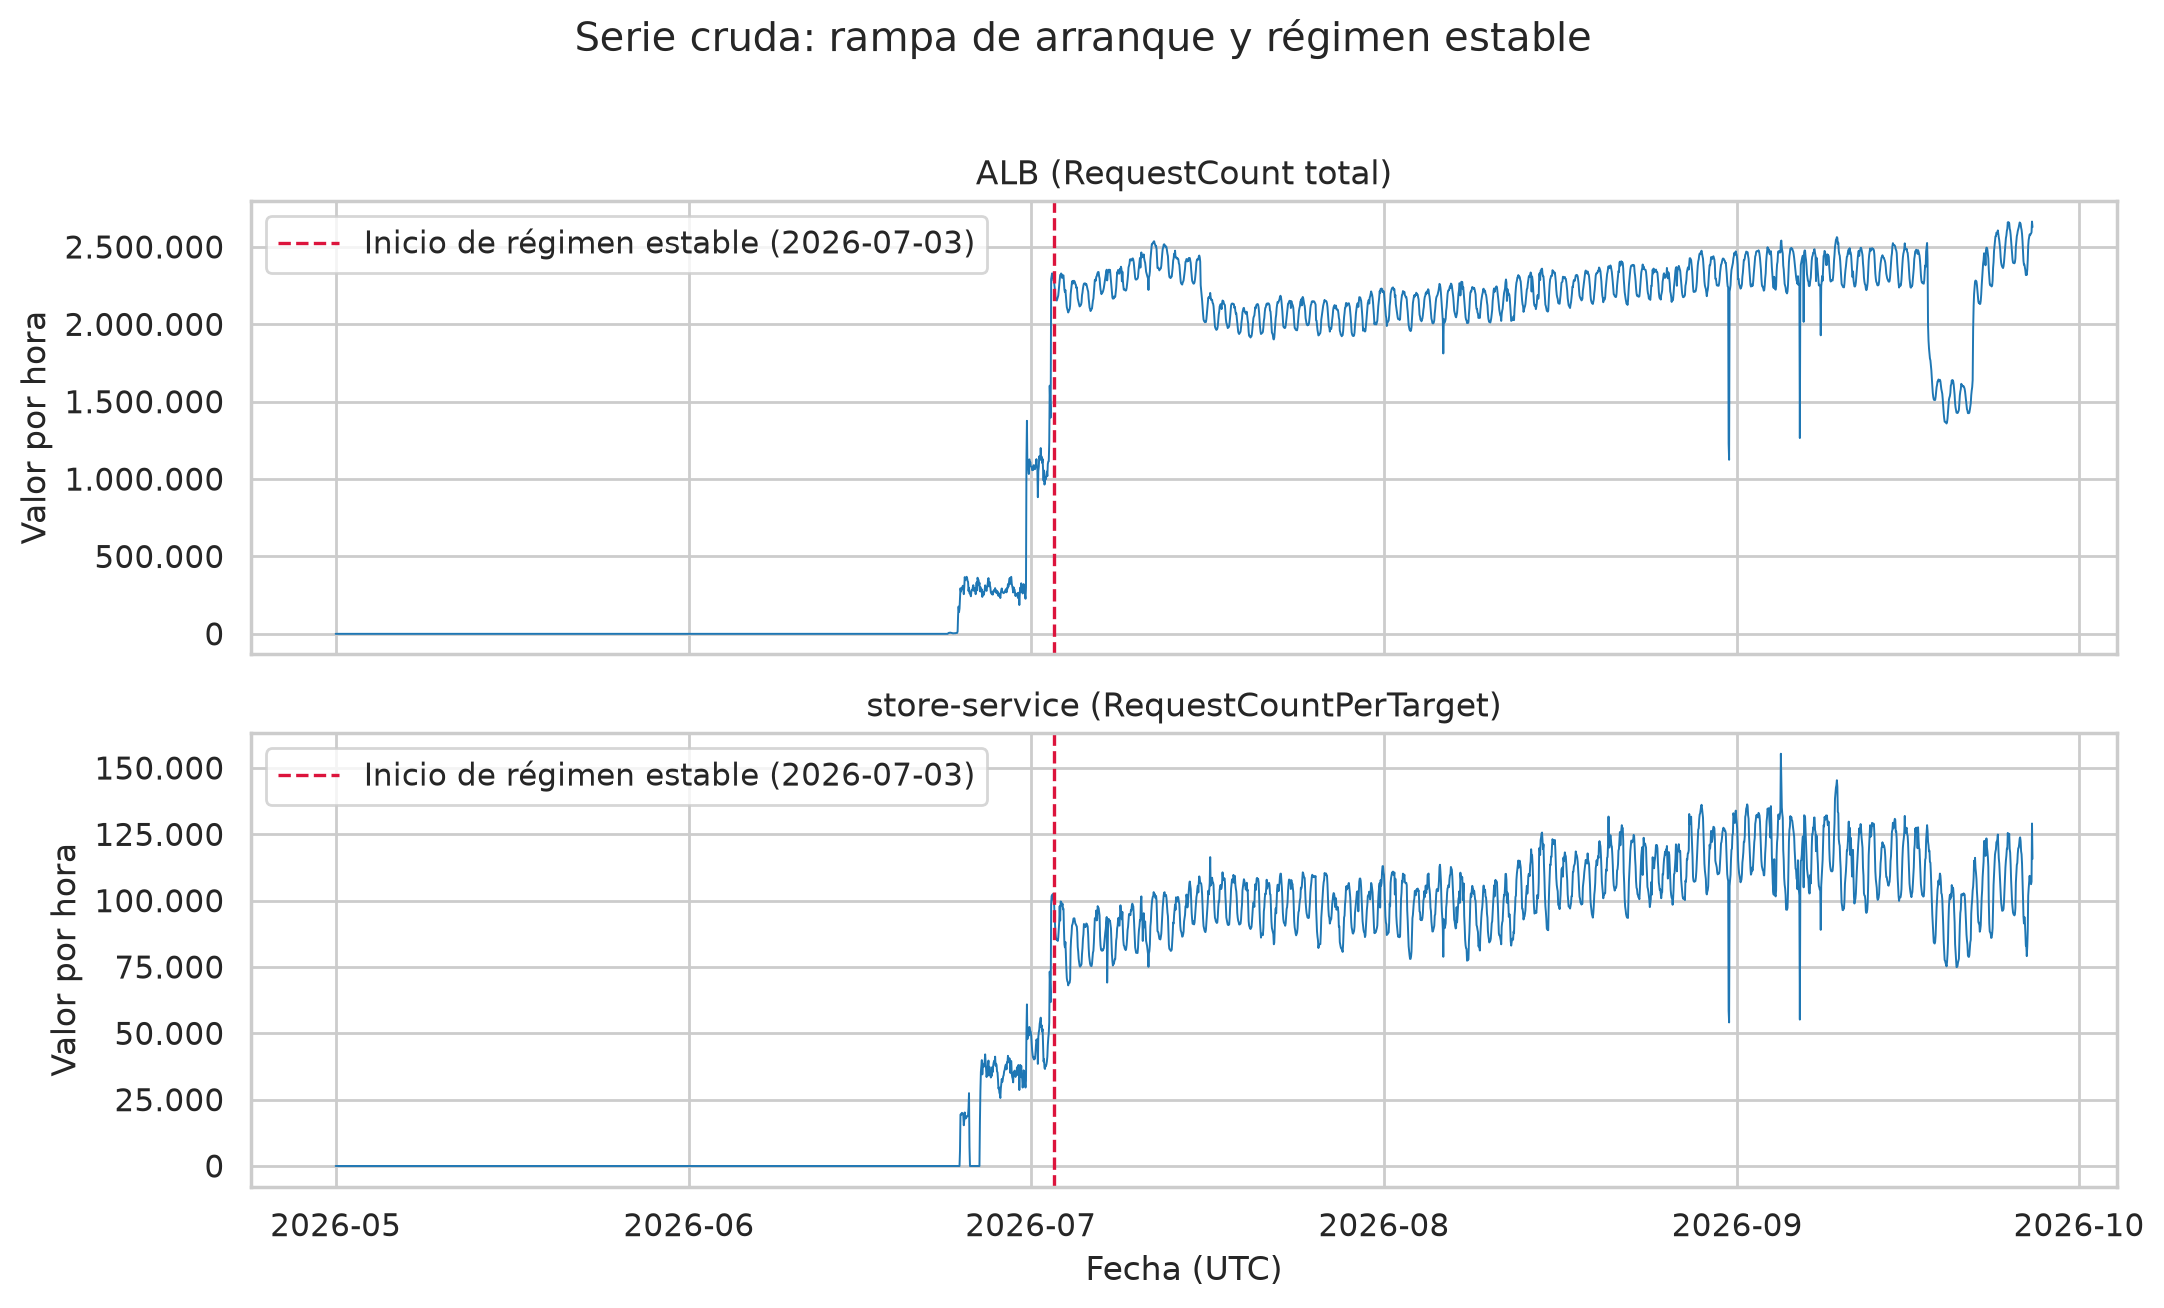
\includegraphics[width=0.85\textwidth]{01_raw_ramp.png}
  \caption{Serie ALB sin procesar, con la rampa de encendido del balanceador previa al 3 de julio de 2026.}
  \label{fig:raw_ramp}
\end{figure}

Sobre la serie transformada (logaritmo más uno), los contrastes de Dickey-Fuller aumentado
\parencite{dickey1979} y de Kwiatkowski-Phillips-Schmidt-Shin \parencite{kwiatkowski1992} coinciden en
rechazar la estacionariedad en niveles para ambas series (ALB: $p_{\text{ADF}}=0,810$,
$p_{\text{KPSS}}=0,010$; store-service: $p_{\text{ADF}}=0,174$, $p_{\text{KPSS}}=0,010$) y en no rechazarla
tras una primera diferencia (ALB: $p_{\text{ADF}}\approx0,000$, $p_{\text{KPSS}}=0,100$; store-service:
$p_{\text{ADF}}\approx0,000$, $p_{\text{KPSS}}=0,100$), lo que justifica el orden de diferenciación de los
modelos ARIMA/SARIMA empleados.

Entre el 17 de septiembre de 2026, 18:00 UTC, y el 22 de septiembre de 2026, 13:00 UTC (116 horas), una
reversión de despliegue redujo transitoriamente el tráfico observado (Figura~\ref{fig:intervencion}). Siguiendo
el tratamiento de eventos exógenos propuesto por \textcite{boxtiao1975}, esta ventana no se descarta ni se
trata como una observación válida del proceso: se imputa reemplazando cada hora por el valor observado en
la misma hora de la semana anterior, corregido por un factor de nivel que preserva el crecimiento
orgánico semana a semana (razón entre el promedio de las 168 horas previas a la intervención y el
promedio de las 168 horas de la semana anterior a esas). Tras la reversión, la serie store-service se
estabiliza en un nivel aproximadamente 7\,\% por debajo del previo a la intervención, atribuible a un
cambio en la cantidad de destinos de balanceo activos; este desplazamiento se trata como parte del proceso
genuino y no se corrige.

\begin{figure}[htbp]
  \centering
  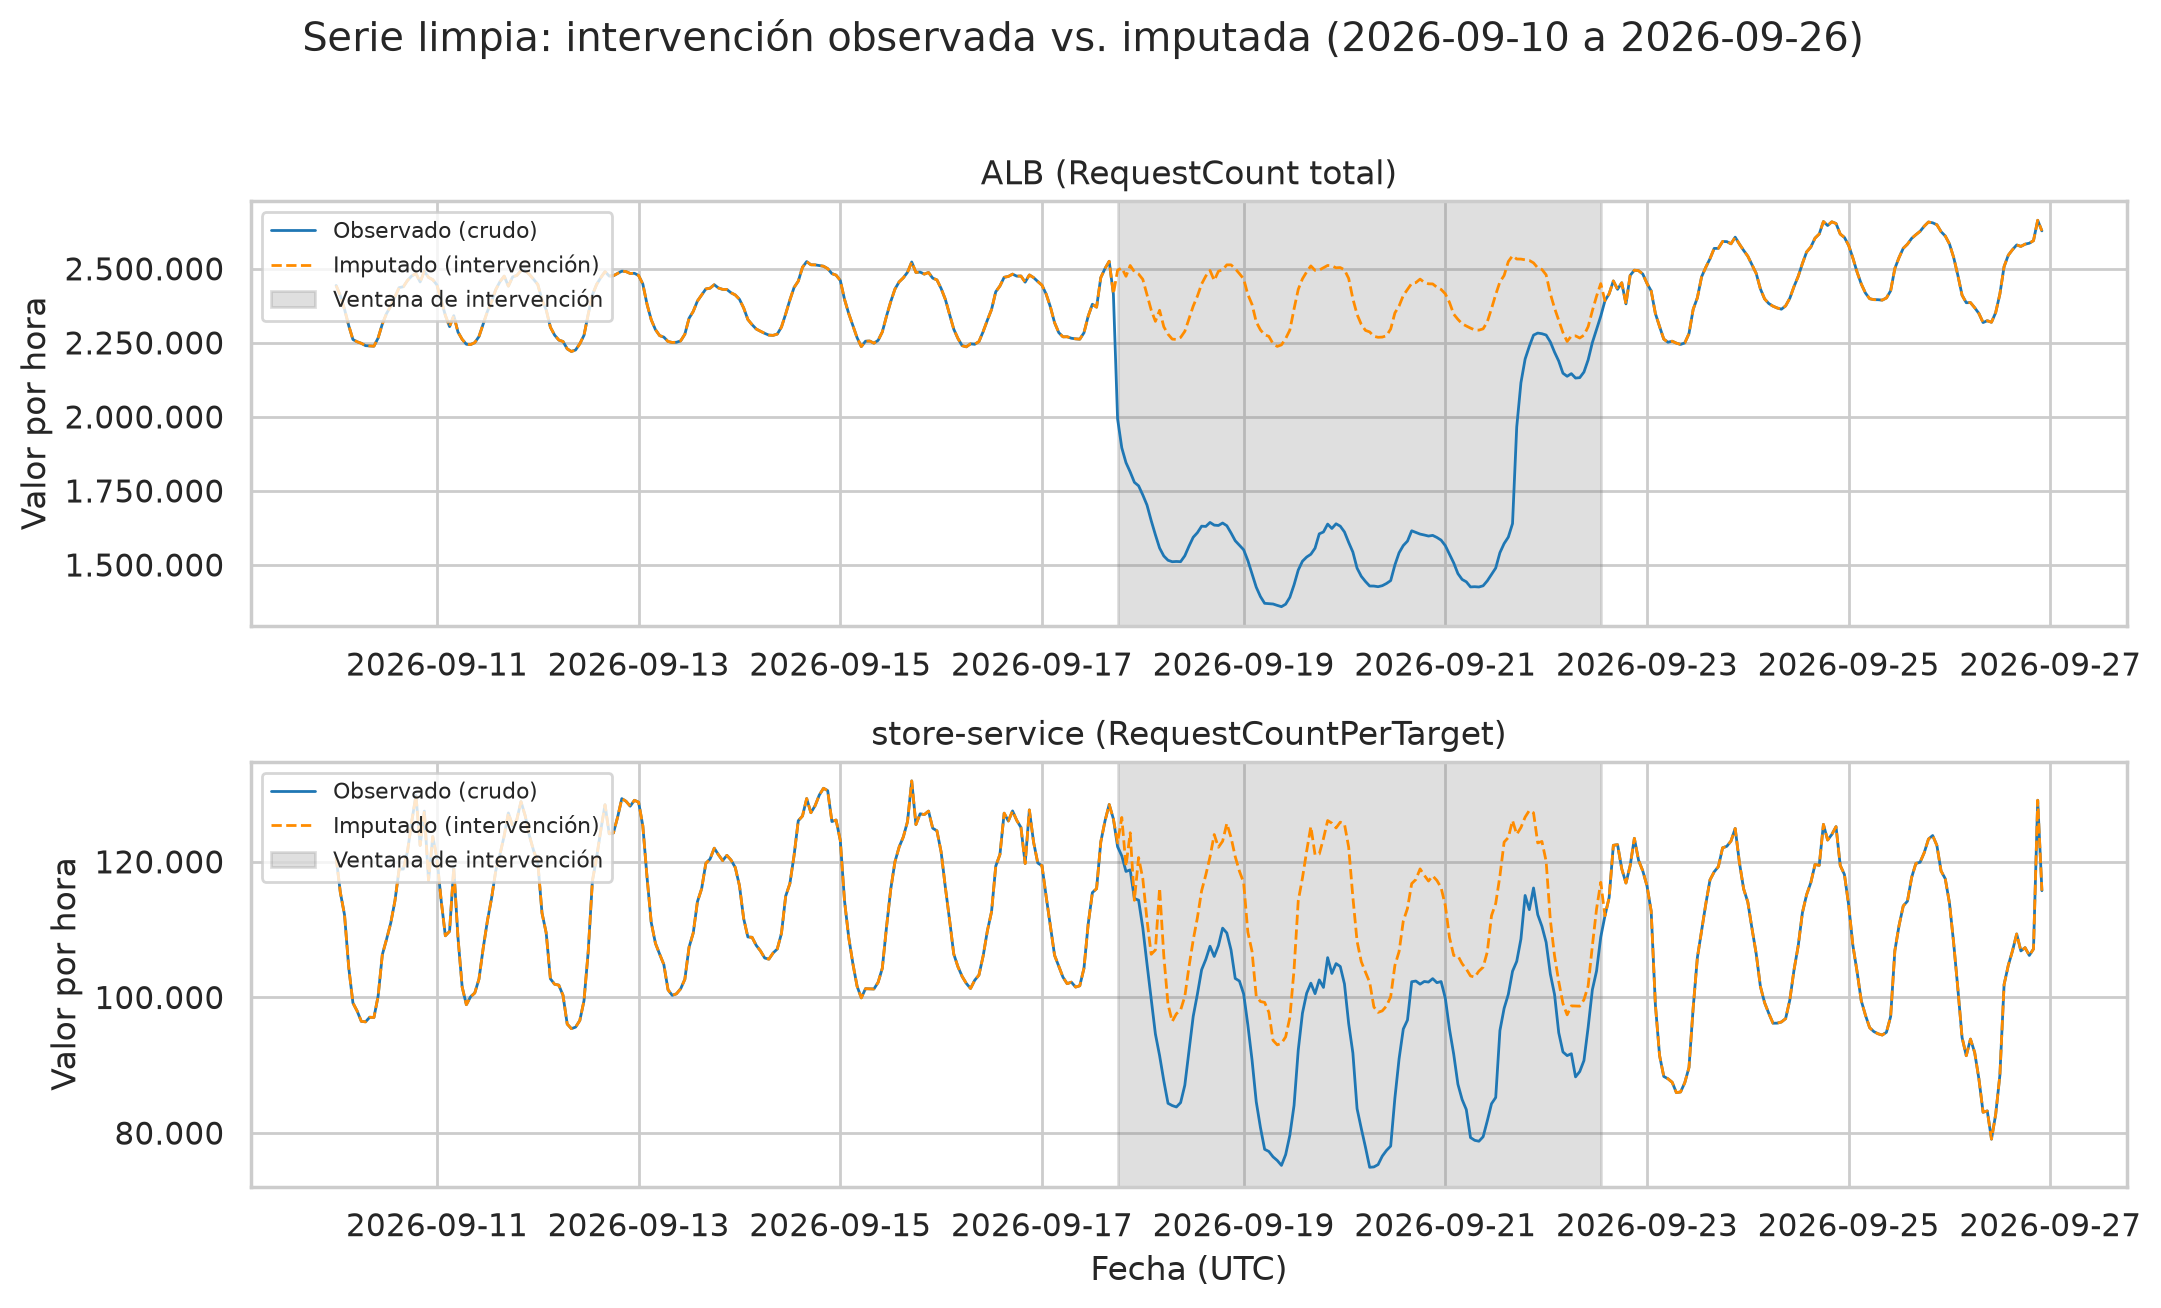
\includegraphics[width=0.85\textwidth]{01_intervention_zoom.png}
  \caption{Detalle de la intervención de despliegue (17 al 22 de septiembre de 2026) en ambas series.}
  \label{fig:intervencion}
\end{figure}

\subsubsection{Variables utilizadas}

Los modelos de Machine Learning se alimentan con rezagos de 1 a 24, 48, 168 y 336 horas, estadísticos
móviles (media y desvío) en ventanas de 24 y 168 horas, y variables de calendario (hora local, día de la
semana, fin de semana, feriado argentino, indicador de intervención). La correlación cruzada entre ambas
series, calculada sobre la serie transformada (logaritmo más uno y primera diferencia), alcanza su máximo
en el rezago cero ($r=0,852$; Apéndice~A), sin evidencia de una relación de adelanto-atraso aprovechable;
por esa razón, ninguna serie se utiliza como variable exógena de la otra. La estacionalidad semanal, con
medias por día de la semana que difieren menos del 3\,\% respecto de la media general en ambas series
(Figura~\ref{fig:weekly}), se considera despreciable frente a la estacionalidad diaria (fuerza estacional
de 0,771 para ALB y 0,846 para store-service, según la descomposición MSTL) y se excluye de los modelos
Prophet, NeuralProphet y del período estacional utilizado por el MASE ($m=24$).

\begin{figure}[htbp]
  \centering
  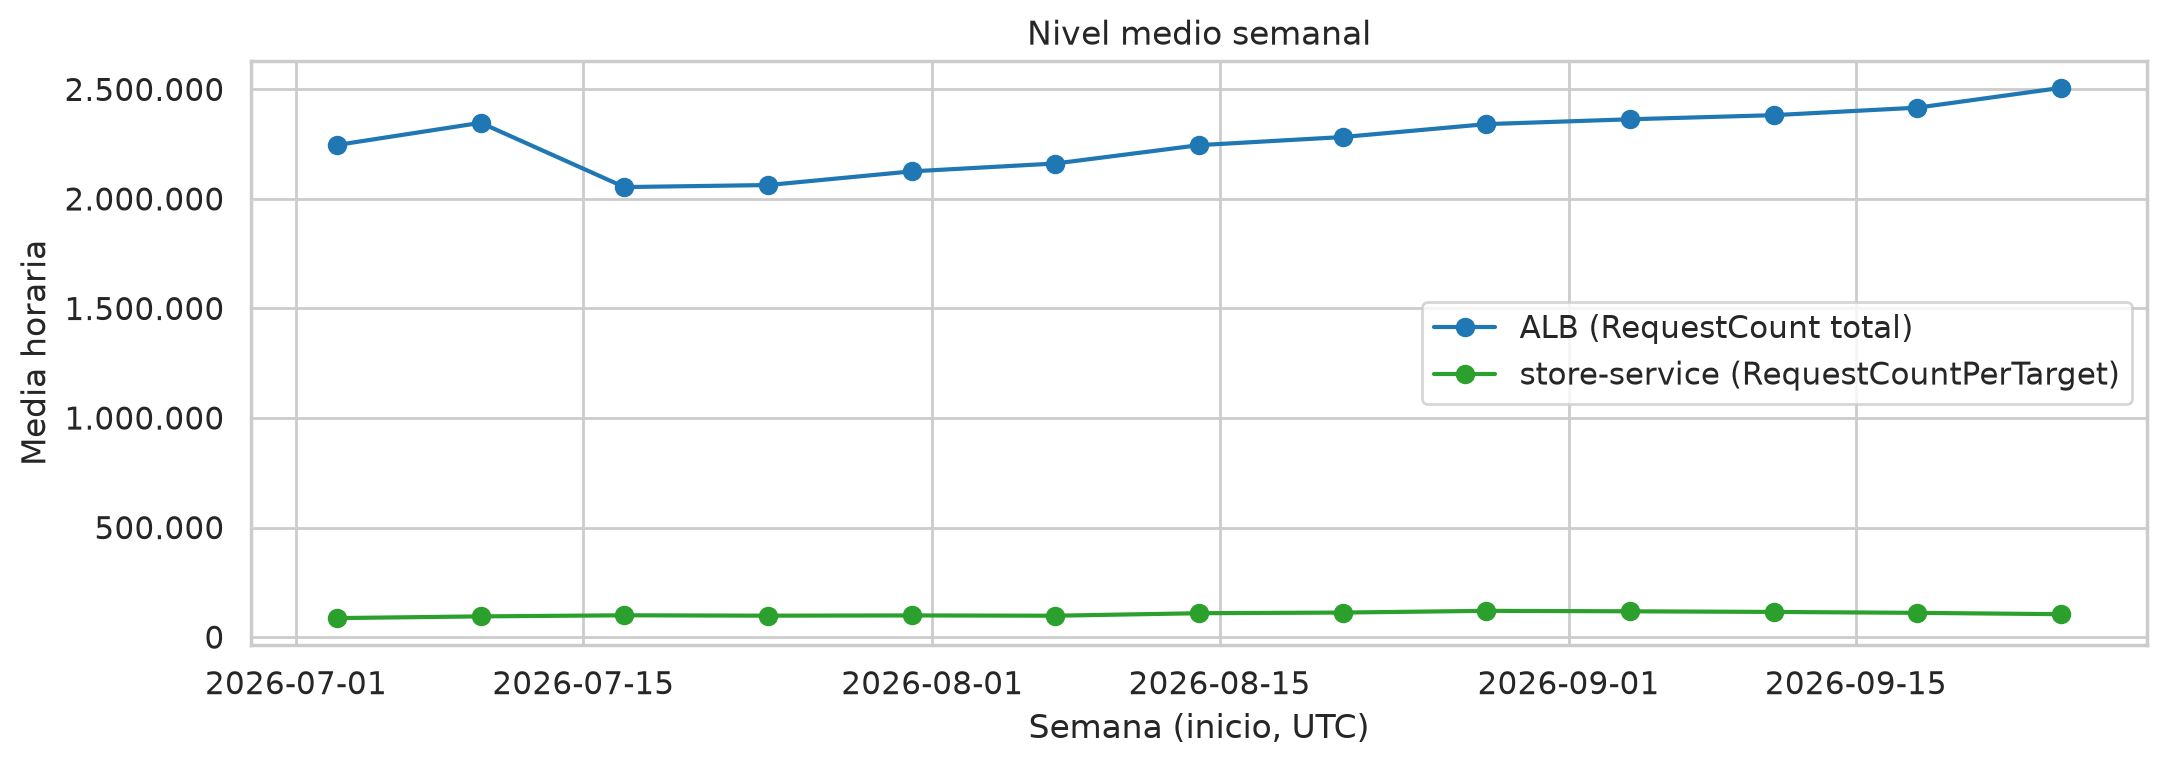
\includegraphics[width=0.8\textwidth]{01_weekly_level.png}
  \caption{Nivel medio por día de la semana, ambas series, historial efectivo.}
  \label{fig:weekly}
\end{figure}

\subsubsection{Esquema de validación y horizonte de prueba}

A diferencia de una validación cruzada expandida de múltiples pliegues, este trabajo adopta una única
ventana de validación de 48 horas (Figura~\ref{fig:split}), decisión justificada por el tiempo total de
cómputo que exige comparar 32 configuraciones por serie. La Tabla~\ref{tab:protocolo} resume las ventanas
del protocolo.

\begin{figure}[htbp]
  \centering
  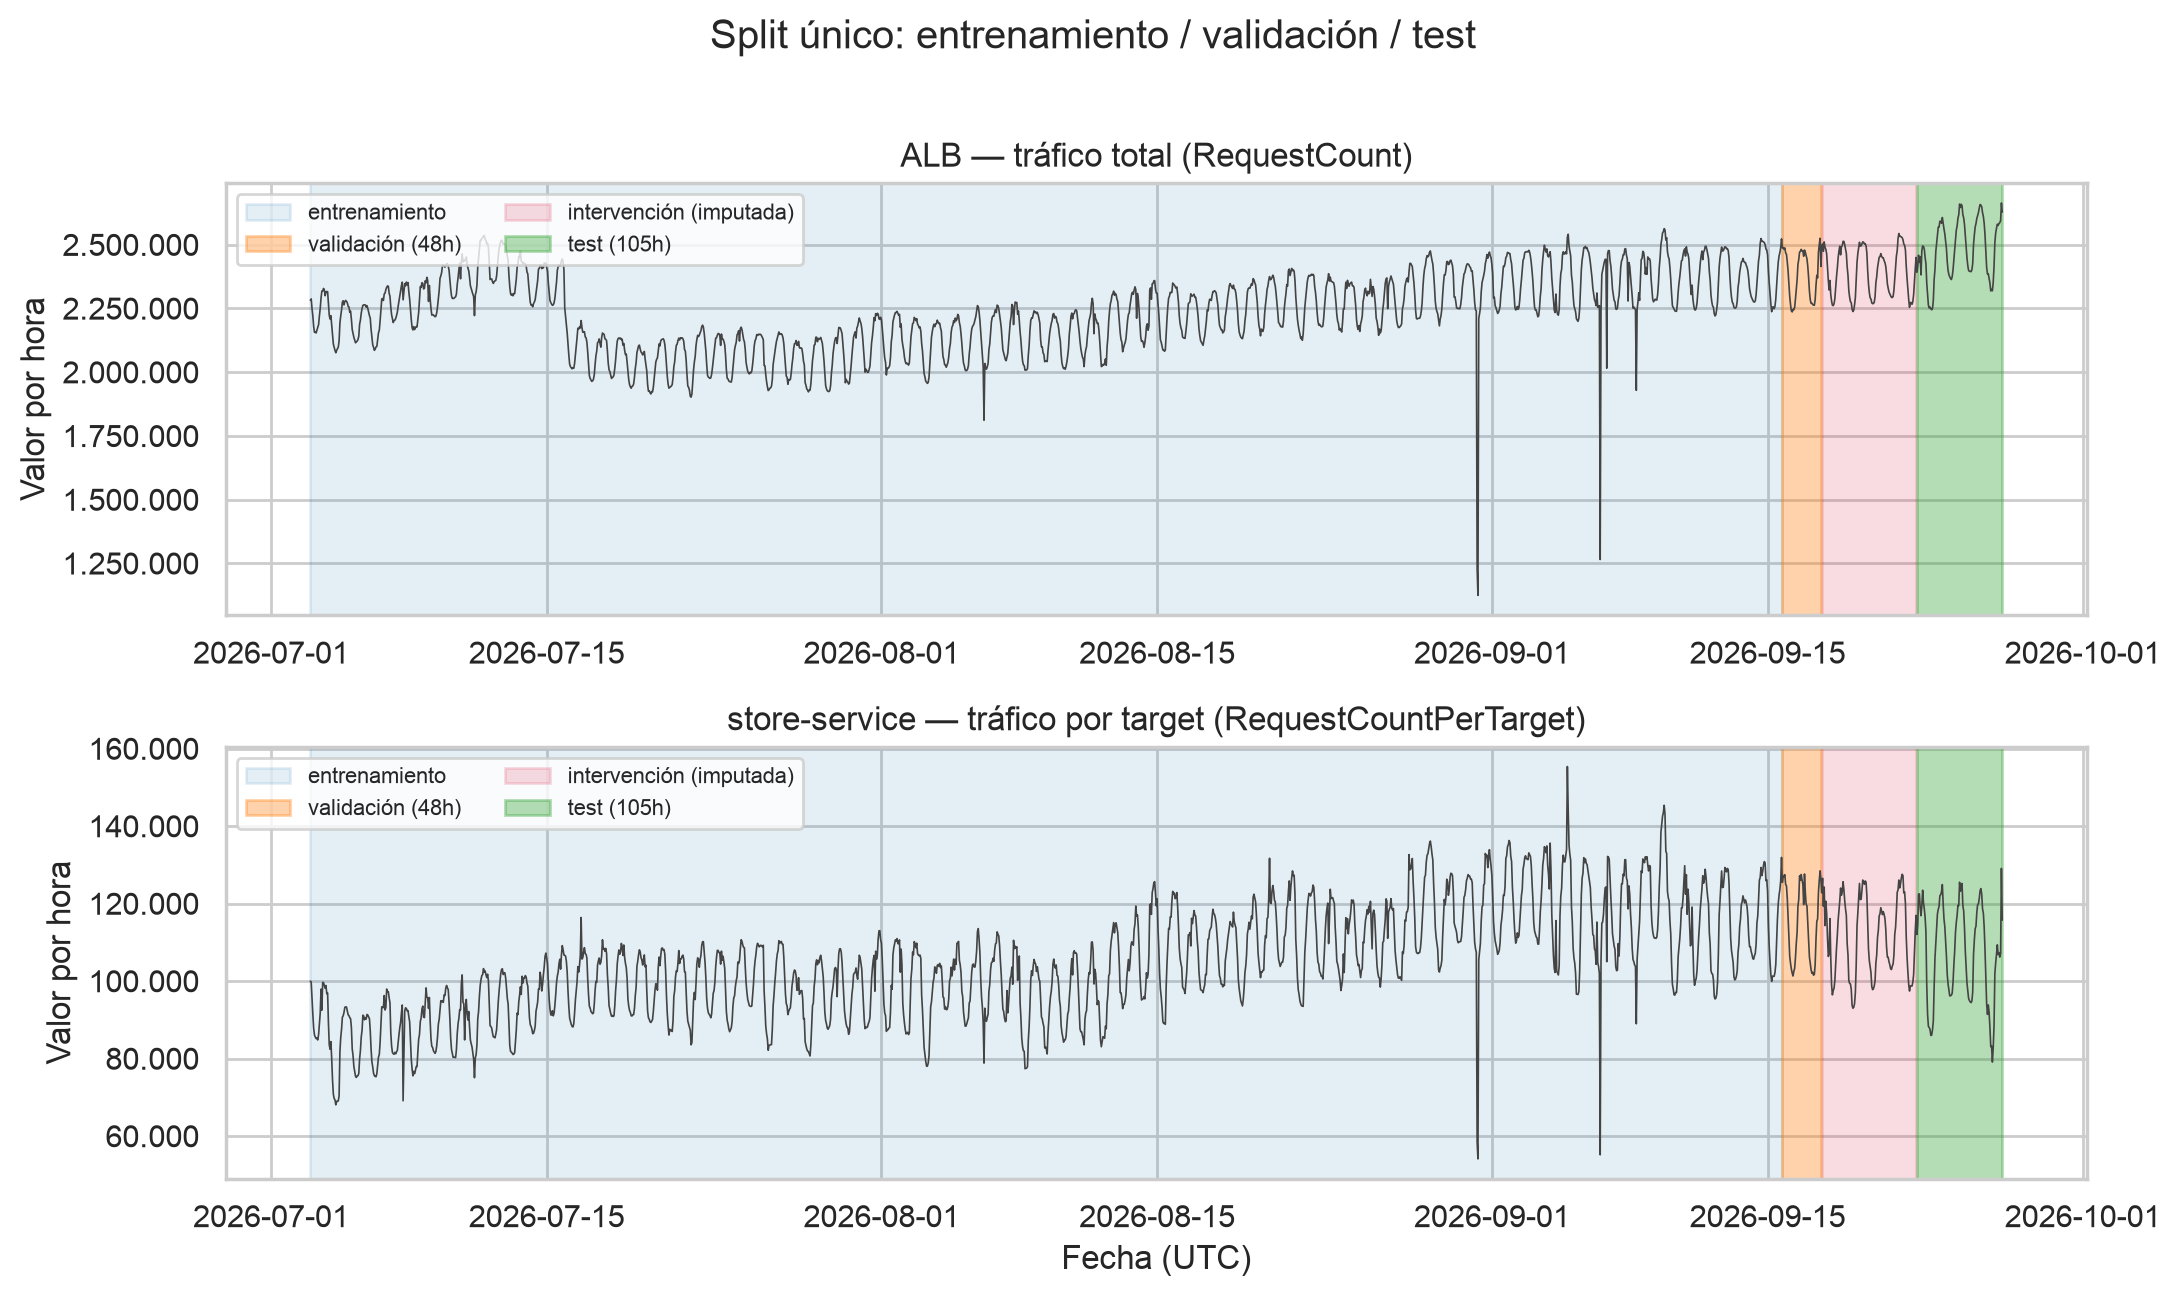
\includegraphics[width=0.92\textwidth]{02_split_train_val_test.png}
  \caption{Esquema de partición temporal en entrenamiento, validación y prueba.}
  \label{fig:split}
\end{figure}

\begin{table}[htbp]
  \centering
  \caption{Ventanas del protocolo de evaluación (todos los horarios en UTC).}
  \label{tab:protocolo}
  \small
  \begin{tabular}{lll}
    \toprule
    Segmento & Rango & Extensión \\
    \midrule
    Historial efectivo & 03/07/2026 00:00 -- 26/09/2026 22:00 & 2.063 h \\
    Ajuste seguro (tuning / \textit{early stopping}) & 168 h previas a la ventana de validación & 168 h \\
    Validación (selección del modelo) & 48 h previas al inicio de la intervención & 48 h \\
    Intervención (imputada) & 17/09/2026 18:00 -- 22/09/2026 13:00 & 116 h \\
    Prueba & 22/09/2026 14:00 -- 26/09/2026 22:00 & 105 h \\
    Pronóstico final & 26/09/2026 23:00 -- 28/09/2026 22:00 & 48 h \\
    \bottomrule
  \end{tabular}
\end{table}

Para evitar la fuga de información señalada en la sección de Marco Teórico, el ajuste de hiperparámetros
de los modelos de Machine Learning y la parada anticipada de las redes profundas se realizan exclusivamente
sobre la ventana de 168 horas previa a la ventana de validación, nunca sobre esta última. El Código~\ref{cod:early_stopping}
ilustra esta separación para las arquitecturas de Deep Learning, junto con la restitución de los pesos de
la mejor época tras la parada anticipada --una corrección aplicada durante el desarrollo del trabajo, que
se documenta más adelante, al tratar los modelos de Deep Learning--.

\begin{lstlisting}[caption={Ajuste con ventana segura de fuga y restitución de la mejor época (\texttt{tsa\_final/dl\_models.py}).}, label=cod:early_stopping]
fit_part = train.iloc[:-ES_WINDOW_HOURS]      # 168 h reservadas
val_part = train.iloc[-(INPUT_CHUNK_LENGTH + ES_WINDOW_HOURS):]

tracker = _BestEpochTracker()
model = self._build(
    n_epochs=MAX_EPOCHS,
    callbacks=[EarlyStopping(monitor="val_loss", patience=PATIENCE, mode="min"), tracker],
)
model.fit(series=fit_ts, val_series=val_ts, verbose=False)
if tracker.best_state is not None:
    model.model.load_state_dict(tracker.best_state)  # no se usan los pesos post-paciencia
\end{lstlisting}

\subsection{Resultados por familia de modelos}

\subsubsection{Referencias ingenuas y modelos estadísticos clásicos}

Las cuatro referencias ingenuas y los cuatro modelos clásicos (Holt-Winters, MSTL con AutoARIMA sobre la
tendencia, AutoARIMA y el SARIMA refit del Trabajo Práctico N.\textsuperscript{o} 1) constituyen el primer
nivel de comparación. En validación, la referencia estacional ingenua ($m=24$) ya resulta muy difícil de
superar: MASE de 0,489 en ALB y de 0,480 en store-service. El AutoARIMA la supera levemente en ALB (0,475)
y queda apenas por encima en store-service (0,532). El SARIMA refit del trabajo anterior, en cambio,
obtiene un MASE de validación considerablemente peor en ambas series (0,923 y 0,647, respectivamente): su
orden fue identificado sobre datos de un mes y una rampa de tráfico distinta, y no se reoptimiza en este
trabajo. Esa desventaja en validación se revierte por completo en el conjunto de prueba, como se discute
más adelante, en la sección de selección del modelo.

\subsubsection{Machine Learning: árboles con boosting y ensambles}
\label{sec:ml}

Con hiperparámetros por defecto, ningún modelo de Machine Learning supera a la referencia estacional
ingenua en validación: el mejor de ellos en ALB (CatBoost, MASE 0,598) y en store-service (Ridge, MASE
1,201) quedan por encima de 0,489 y 0,480, respectivamente. Solo tras ajustar hiperparámetros con Optuna
--sobre la misma ventana de 48 horas luego utilizada para clasificar los modelos-- tres configuraciones de
ALB (CatBoost, Random Forest y LightGBM ajustados) logran un MASE de validación inferior a la referencia
ingenua (0,353, 0,416 y 0,421, respectivamente); en store-service, ninguna configuración ajustada alcanza
ese umbral (mínimo de 0,573 con LightGBM ajustado). Estos cinco modelos se marcan como \emph{contaminados}
en este trabajo, dado que su puntaje de validación es optimista por construcción: fueron optimizados sobre
la misma ventana que luego los clasifica. El efecto es visible en el conjunto de prueba: CatBoost ajustado,
el mejor de ALB en validación, cae al puesto 17 de 32 en prueba (MASE 2,313), y Random Forest ajustado
resulta, dentro de esta familia, el de peor desempeño relativo en prueba dentro de la serie ALB (MASE 3,455,
frente a 0,416 en validación). El \emph{stacking} de los tres mejores modelos ajustados, por su parte,
resulta el peor modelo de toda la familia de Machine Learning en ambas series y en ambos conjuntos (MASE de
prueba de 4,989 en ALB y 1,981 en store-service), lo que sugiere que combinar modelos ya sobreajustados a
la ventana de validación no mitiga, sino que propaga, ese sobreajuste. La Figura~\ref{fig:shap} muestra que
los rezagos de 1, 2, 23, 24 y 48 horas dominan la importancia de las variables según SHAP, muy por delante
de los rezagos semanales (168 horas), lo que es consistente con la estacionalidad diaria dominante
documentada en la sección de preparación de datos.

\begin{figure}[htbp]
  \centering
  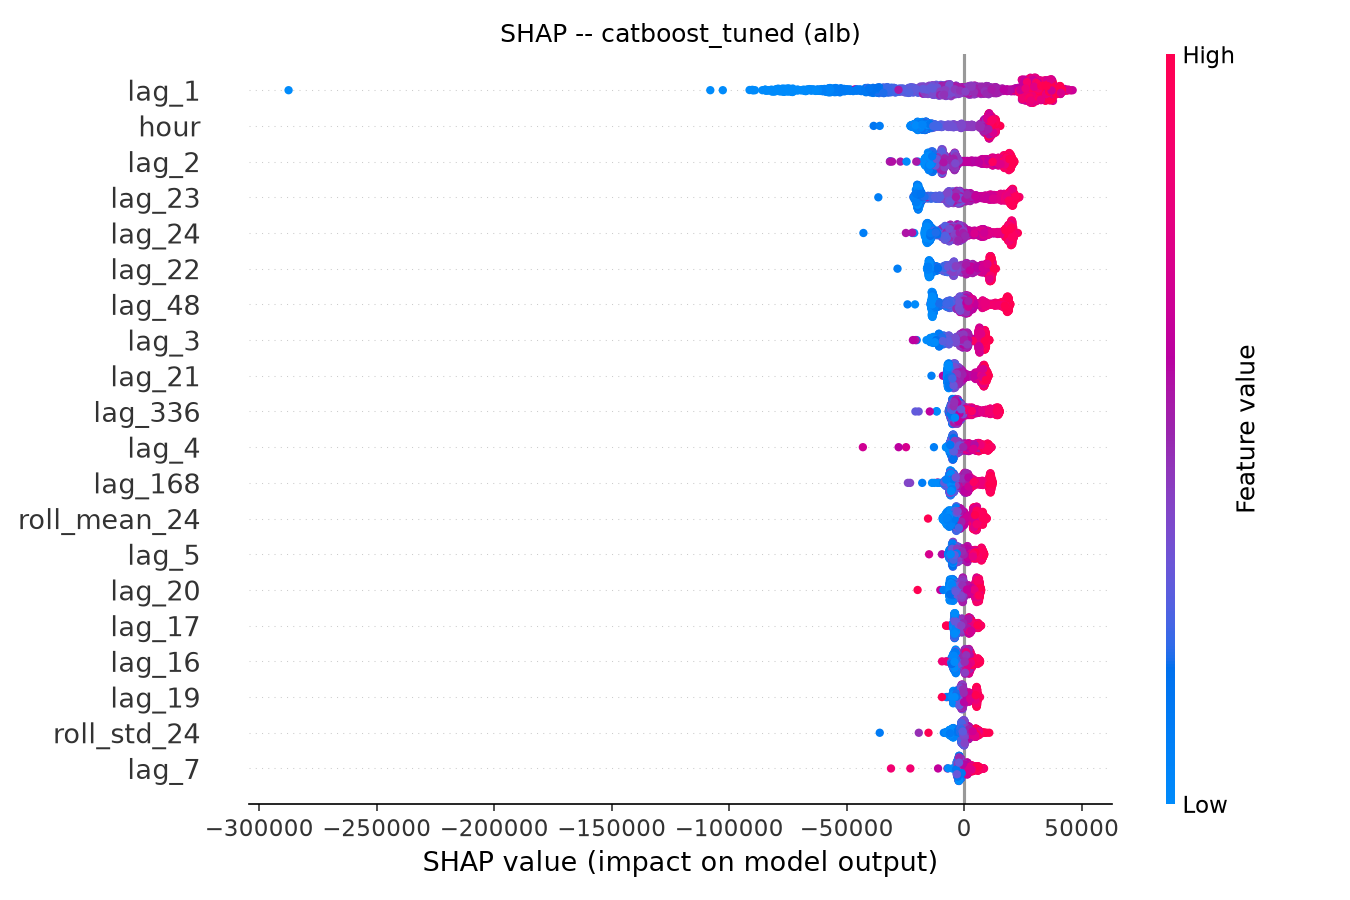
\includegraphics[width=0.85\textwidth]{03_shap_alb.png}
  \caption{Importancia de variables (SHAP) del mejor modelo de Machine Learning, serie ALB.}
  \label{fig:shap}
\end{figure}

\subsubsection{Deep Learning}
\label{sec:dl}

El desarrollo de las seis arquitecturas de Deep Learning reveló un defecto metodológico corregido antes de
la selección final: el mecanismo de parada anticipada de la librería Darts conserva los pesos de la última
época evaluada, no los de la época de menor error de validación, mientras que el ajuste final sobre prueba
entrena exactamente la cantidad de épocas de la mejor época. La primera corrida comparaba, en consecuencia,
un modelo sobreentrenado en validación contra un modelo correctamente detenido en prueba. La corrección
--restituir explícitamente los pesos de la mejor época tras la parada anticipada, documentada en el
Código~\ref{cod:early_stopping}-- se aplicó a las 24 combinaciones de arquitectura, serie y semilla con
parada anticipada, y modificó únicamente los puntajes de validación; los de prueba permanecen sin cambios,
salvo en tres ajustes de TFT en los que el mecanismo de atención, no determinístico en GPU, produjo una
mejor época distinta entre corridas. La Tabla~\ref{tab:dl_correccion} resume el efecto de la corrección
sobre el MASE de validación promediado entre las dos semillas utilizadas.

\begin{table}[htbp]
  \centering
  \caption{MASE de validación antes y después de la corrección de pesos, por arquitectura de Deep Learning.}
  \label{tab:dl_correccion}
  \small
  \begin{tabular}{lrrrr}
    \toprule
    & \multicolumn{2}{c}{ALB} & \multicolumn{2}{c}{store-service} \\
    Arquitectura & Antes & Corregido & Antes & Corregido \\
    \midrule
    LSTM   & 2,337 & 1,909 & 1,017 & 0,728 \\
    N-BEATS & 1,119 & 0,980 & 1,444 & \textbf{0,638} \\
    N-HiTS  & 0,875 & \textbf{0,556} & 1,097 & 0,689 \\
    TCN     & 2,323 & 1,153 & 0,760 & 0,732 \\
    TFT     & 1,516 & 1,535 & 1,342 & 1,083 \\
    TiDE    & 0,998 & 0,790 & 1,211 & 0,862 \\
    \bottomrule
  \end{tabular}
  \\[2pt]
  \footnotesize Se destaca en negrita el mejor MASE corregido de cada serie (N-HiTS en ALB, N-BEATS en
  store-service).
\end{table}

Ninguna arquitectura de Deep Learning supera a la referencia estacional ingenua en validación tras la
corrección, aunque la distancia se reduce sustancialmente respecto de la primera corrida (por ejemplo,
N-HiTS pasa de 0,875 a 0,556 en ALB). En el conjunto de prueba, N-BEATS resulta el mejor modelo de Deep
Learning en ambas series (MASE de 1,744 en ALB y 1,247 en store-service), aunque no el mejor modelo del
proyecto completo (sección de selección del modelo, más adelante). El caso más notorio es el de LSTM en ALB: la mejor época,
para ambas semillas, es la primera (Tabla~\ref{tab:mejor_epoca}), un resultado reproducido de forma idéntica
antes y después de la corrección y que se interpreta como un hallazgo genuino --el modelo prácticamente no
llega a entrenarse antes de que la pérdida de validación comience a degradarse-- y no como un artefacto de
implementación; en prueba, esta arquitectura resulta el peor modelo de las 32 configuraciones evaluadas
para ALB (MASE de 7,817, último puesto). El Transformer de fusión temporal (TFT), por su parte, nunca ocupa
el primer puesto en ninguna serie ni conjunto, pese a exigir el mayor costo de entrenamiento de todo el
proyecto (sección de costo computacional, más adelante).

\begin{table}[htbp]
  \centering
  \caption{Mejor época (de un máximo de 100, paciencia 12) por arquitectura, serie y semilla.}
  \label{tab:mejor_epoca}
  \small
  \begin{tabular}{lrrr}
    \toprule
    Arquitectura & Serie & Semilla 42 & Semilla 43 \\
    \midrule
    LSTM   & ALB            & 1  & 1  \\
    N-BEATS & ALB           & 83 & 97 \\
    N-HiTS  & ALB           & 21 & 42 \\
    LSTM   & store-service  & 18 & 17 \\
    N-BEATS & store-service & 34 & 45 \\
    \bottomrule
  \end{tabular}
\end{table}

\subsubsection{Prophet, modelos híbridos, AutoML y modelo de fundación}

La Figura~\ref{fig:hibridos} presenta el MASE de validación de las ocho configuraciones de esta fase. El
ensamble de ponderación uniforme (\emph{equal-weight}, contaminado por construcción, ya que sus miembros se
eligen con el mismo MASE de validación que este puntaje mide) encabeza la clasificación de ALB (0,404) y
prácticamente iguala a la referencia ingenua en store-service (0,480126 frente a 0,480171). Entre los
modelos no contaminados, Prophet sin ajuste de hiperparámetros resulta el más competitivo de la fase en
ambas series (0,532 y 0,506, respectivamente), mientras que AutoGluon TimeSeries se aproxima en ALB
(0,499). El híbrido de descomposición MSTL seguido de LightGBM sobre la serie desestacionalizada constituye
el fracaso más marcado de esta fase: en store-service alcanza el peor MASE de validación de las ocho
configuraciones (1,848) y, en prueba, el peor resultado de las 32 configuraciones evaluadas para esa serie
(MASE de 3,100, último puesto de 32); en ALB su MASE de prueba (5,721) también es de los más altos del
proyecto (puesto 30 de 32). Este comportamiento es consistente con una deriva recursiva: al reconstruir la
componente estacional futura repitiendo los últimos 24 valores observados, cualquier error del componente
LightGBM sobre la tendencia se acumula sin corrección a lo largo del horizonte de prueba.

\begin{figure}[htbp]
  \centering
  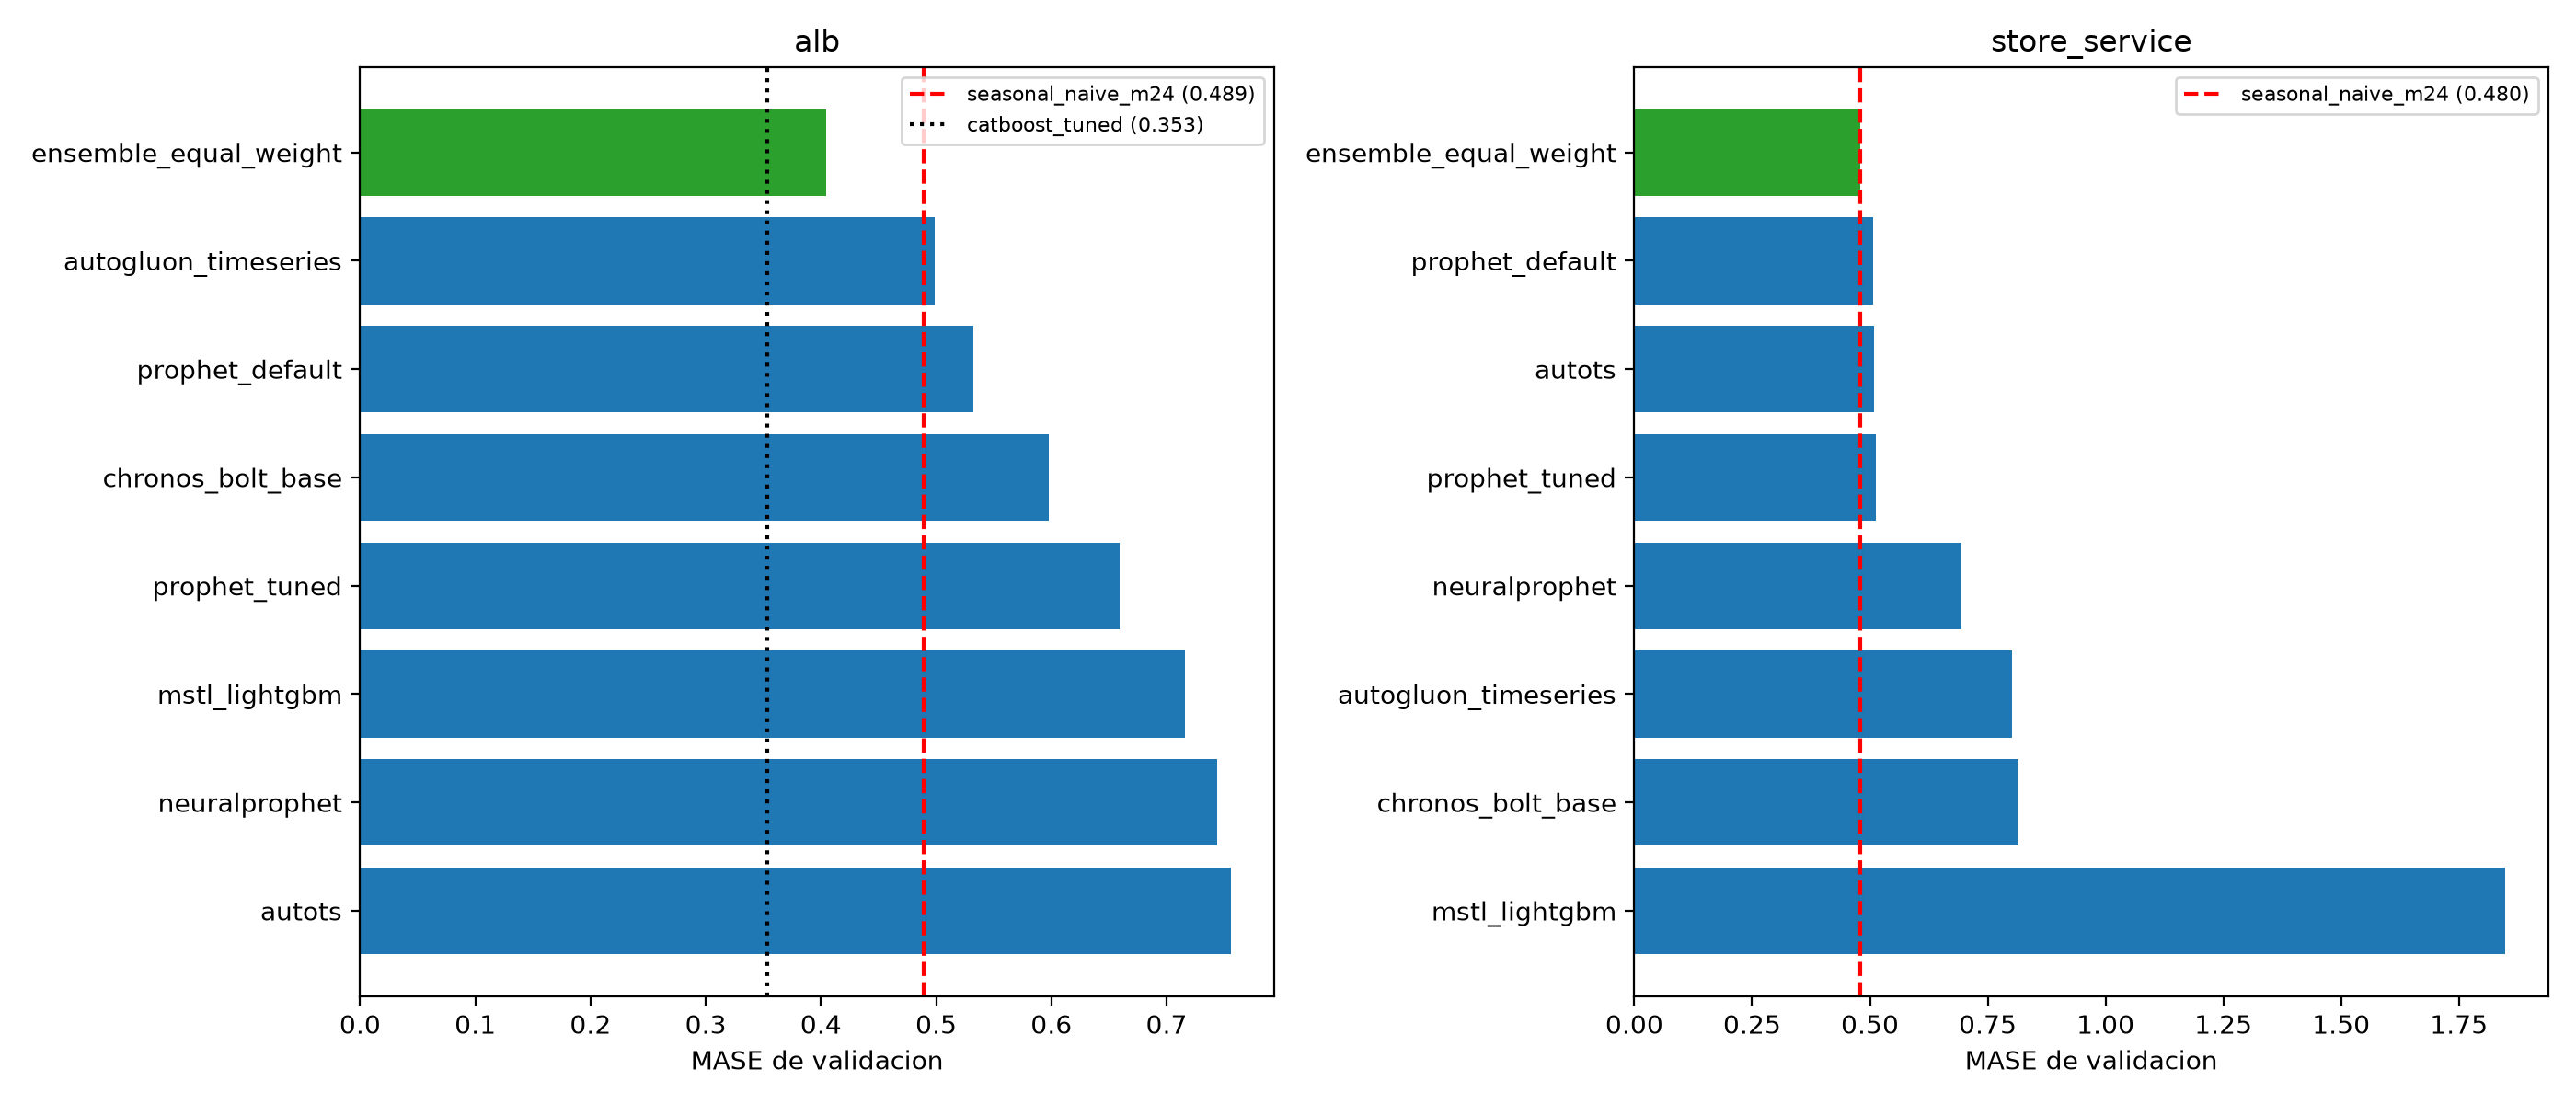
\includegraphics[width=0.9\textwidth]{05_val_mae_ranking.png}
  \caption{MASE de validación, modelos de Prophet, híbridos, AutoML y de fundación.}
  \label{fig:hibridos}
\end{figure}

Chronos, evaluado en modalidad de inferencia directa sin ajuste alguno sobre las series propias, obtiene un
MASE de validación intermedio en ambas series (0,598 en ALB, 0,816 en store-service), un resultado
razonable para un modelo que nunca observó estas series durante su preentrenamiento. Su intervalo de
predicción, sin embargo, solo cubre los cuantiles 0,1 y 0,9 sobre los que fue entrenado: el intervalo del
95\,\% se deja explícitamente sin definir en el pronóstico final, en lugar de aproximarlo con un cuantil
para el que el modelo no fue entrenado.

\subsubsection{Comparación entre familias}

La Figura~\ref{fig:familias} resume el mejor MASE de validación logrado por cada familia de modelos, en
ambas series. Las Tablas~\ref{tab:comparacion_alb} y~\ref{tab:comparacion_store} presentan, de forma
compacta, el mejor modelo de cada familia junto con el modelo seleccionado, el peor modelo elegible, el
SARIMA refit del trabajo anterior y Chronos; las 32 configuraciones completas de cada serie se listan en el
Apéndice~A.

\begin{figure}[htbp]
  \centering
  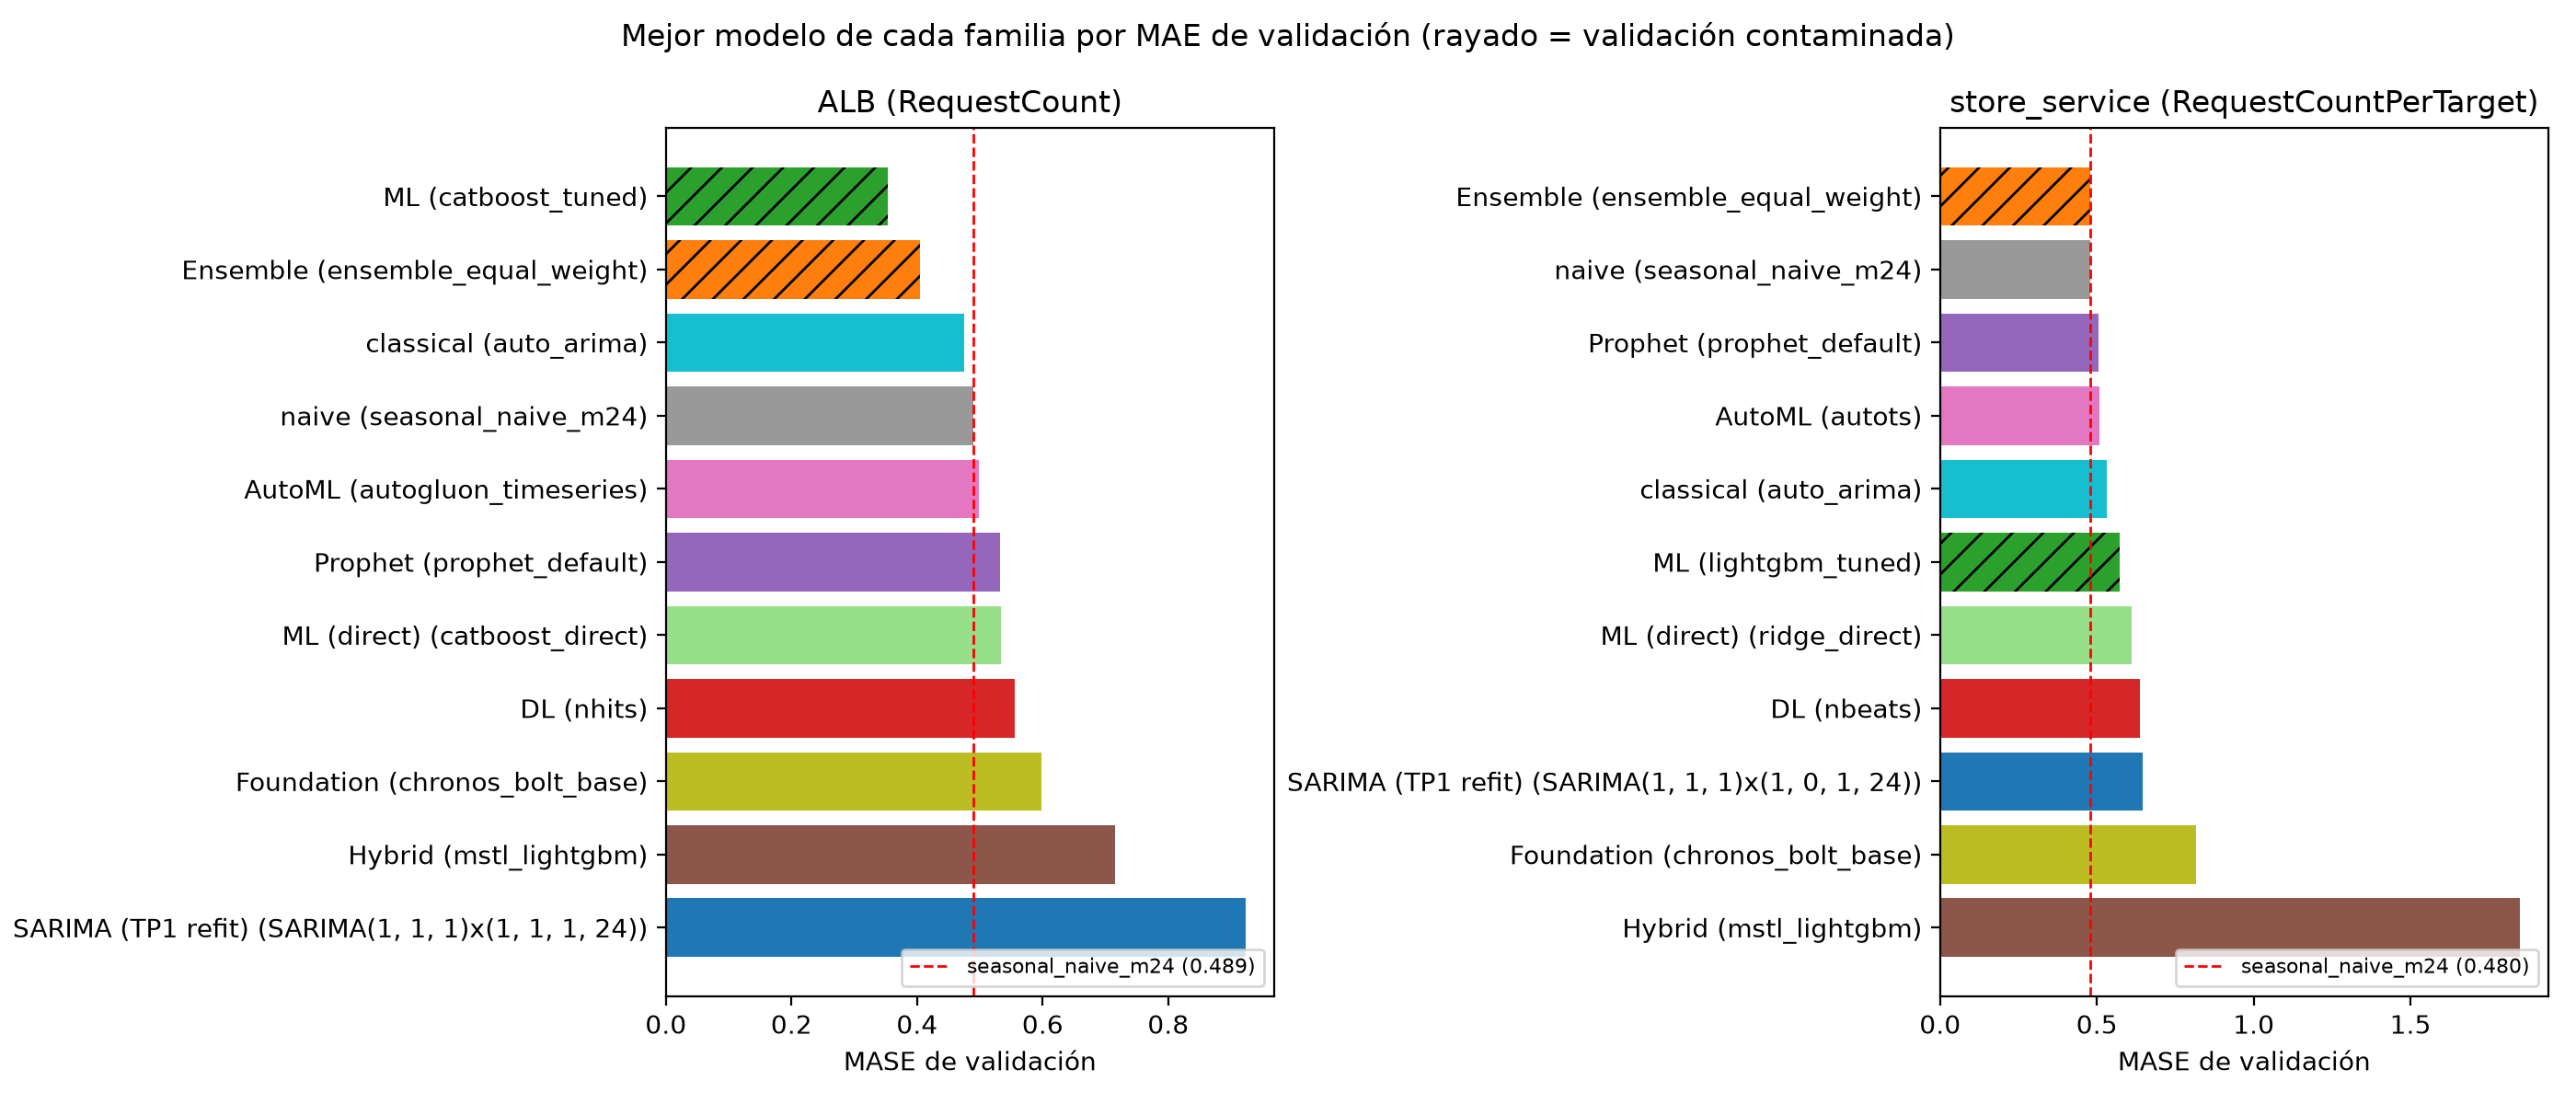
\includegraphics[width=0.85\textwidth]{06_best_per_family.png}
  \caption{Mejor MASE de validación por familia de modelos, ambas series.}
  \label{fig:familias}
\end{figure}

\begin{table}[htbp]
  \centering
  \caption{Comparación compacta de modelos -- serie ALB (MAE en unidades de la serie; MASE adimensional).}
  \label{tab:comparacion_alb}
  \small
  \begin{tabular}{llrrr}
    \toprule
    Modelo & Familia & MAE val. & MASE val. & MASE prueba \\
    \midrule
    \textbf{auto\_arima (seleccionado)} & Clásico & 18.807,50 & \textbf{0,475} & 2,058 \\
    seasonal\_naive\_m24 & Ingenuo & 19.369,02 & 0,489 & 1,990 \\
    SARIMA (TP1 refit) & Fundacional TP1 & 36.524,57 & 0,923 & \textbf{1,526} \\
    catboost\_tuned\textsuperscript{a} & ML & 13.994,36 & 0,353 & 2,313 \\
    catboost\_direct & ML (directo) & 21.126,48 & 0,534 & 2,364 \\
    nhits & DL & 22.021,71 & 0,556 & 2,441 \\
    prophet\_default & Prophet & 21.066,96 & 0,532 & 2,065 \\
    mstl\_lightgbm & Híbrido & 28.341,14 & 0,716 & 5,721 \\
    autogluon\_timeseries & AutoML & 19.748,53 & 0,499 & 1,974 \\
    chronos\_bolt\_base & Fundación & 23.678,74 & 0,598 & 2,007 \\
    ensemble\_equal\_weight\textsuperscript{a} & Ensamble & 16.006,29 & 0,404 & 2,352 \\
    average & Peor elegible & 149.950,95 & 3,788 & 6,011 \\
    \bottomrule
  \end{tabular}
  \\[2pt]
  \footnotesize\textsuperscript{a}Puntaje de validación contaminado; no elegible para la selección.
\end{table}

\begin{table}[htbp]
  \centering
  \caption{Comparación compacta de modelos -- serie store-service.}
  \label{tab:comparacion_store}
  \small
  \begin{tabular}{llrrr}
    \toprule
    Modelo & Familia & MAE val. & MASE val. & MASE prueba \\
    \midrule
    \textbf{seasonal\_naive\_m24 (seleccionado)} & Ingenuo & 2.281,85 & \textbf{0,480} & 1,443 \\
    auto\_arima & Clásico & 2.525,88 & 0,532 & 1,408 \\
    SARIMA (TP1 refit) & Fundacional TP1 & 3.075,43 & 0,647 & 1,426 \\
    lightgbm\_tuned\textsuperscript{a} & ML & 2.723,67 & 0,573 & 1,770 \\
    ridge\_direct & ML (directo) & 2.905,15 & 0,611 & 1,840 \\
    nbeats & DL & 3.031,39 & 0,638 & 1,247 \\
    prophet\_default & Prophet & 2.405,88 & 0,506 & 1,083 \\
    neuralprophet & Prophet & 3.297,54 & 0,694 & \textbf{1,071} \\
    mstl\_lightgbm & Híbrido & 8.779,73 & 1,848 & 3,100 \\
    autots & AutoML & 2.412,97 & 0,508 & 1,596 \\
    chronos\_bolt\_base & Fundación & 3.877,73 & 0,816 & 1,673 \\
    ensemble\_equal\_weight\textsuperscript{a} & Ensamble & 2.281,64 & 0,480 & 1,612 \\
    drift & Peor elegible & 17.022,66 & 3,582 & 2,587 \\
    \bottomrule
  \end{tabular}
  \\[2pt]
  \footnotesize\textsuperscript{a}Puntaje de validación contaminado; no elegible para la selección. Se
  incluye NeuralProphet además del mejor Prophet por ser, con amplio margen, el mejor modelo de prueba de
  toda la serie (ver la sección siguiente, de selección del modelo).
\end{table}

\subsection{Selección del modelo y consistencia entre validación y prueba}
\label{sec:seleccion}

La regla de selección adoptada (Código~\ref{cod:seleccion}) recorre el conjunto de 32 modelos por serie,
descarta los marcados como contaminados y selecciona el de menor MAE de validación entre los restantes.
Se marcan como contaminados los cinco modelos ajustados con Optuna sobre la ventana de validación en cada
serie (\texttt{catboost\_tuned}, \texttt{random\_forest\_tuned} y \texttt{lightgbm\_tuned} en ALB;
\texttt{ridge\_tuned}, \texttt{lightgbm\_tuned} y \texttt{xgboost\_tuned} en store-service), el
\emph{stacking} construido a partir de esos modelos ajustados, y el ensamble de ponderación uniforme, cuyos
miembros se eligen con el propio MAE de validación. Prophet ajustado (\texttt{prophet\_tuned}) se excluye de
esta lista porque su ajuste se realiza sobre la ventana segura de 168 horas descrita en la sección de
preparación de datos, nunca sobre la ventana de validación.

\begin{lstlisting}[caption={Regla de selección: menor MAE de validación entre los modelos elegibles (\texttt{tsa\_final/selection.py}).}, label=cod:seleccion]
def select_model(pool: pd.DataFrame, series: str) -> SelectionResult:
    """El modelo seleccionado es el de menor MAE de validacion entre los
    elegibles (la regla adoptada). El conjunto de prueba nunca se usa para
    seleccionar."""
    elig = eligible_val(pool, series)
    return SelectionResult(series=series, selected=elig.iloc[0],
                            runner_up=elig.iloc[1], worst=elig.iloc[-1])
\end{lstlisting}

Bajo esta regla, el modelo seleccionado para ALB es \texttt{auto\_arima} y para store-service es la propia
referencia estacional ingenua. La comparación contra el SARIMA refit del trabajo anterior arroja una mejora
del 48,5\,\% en validación para ALB (MASE de 0,475 frente a 0,923) y del 25,8\,\% en validación para
store-service (0,480 frente a 0,647); en ambos casos, esa ventaja se revierte en el conjunto de prueba: el
modelo seleccionado resulta un 34,9\,\% peor que el SARIMA refit en ALB y un 1,2\,\% peor en store-service.
Comparado contra la referencia estacional ingenua, el modelo seleccionado de ALB mejora un 2,9\,\% en
validación pero empeora un 3,4\,\% en prueba.

La Figura~\ref{fig:consistencia} y el coeficiente de correlación de Spearman entre el orden de validación y
el orden de prueba cuantifican esta divergencia: para ALB, considerando las 32 configuraciones, $\rho=0,237$
($p=0,192$), no significativo al 5\,\%; restringido a los 27 modelos elegibles, $\rho=0,346$ ($p=0,077$),
tampoco significativo. Para store-service, en cambio, la consistencia es moderada y estadísticamente
significativa: $\rho=0,654$ ($p<0,001$) sobre las 32 configuraciones, y $\rho=0,692$ ($p<0,001$) sobre las
27 elegibles. Esta significancia agregada, sin embargo, no impide divergencias puntuales severas: NeuralProphet,
decimocuarto en validación de store-service, resulta el mejor modelo de prueba de toda la serie.

\begin{figure}[htbp]
  \centering
  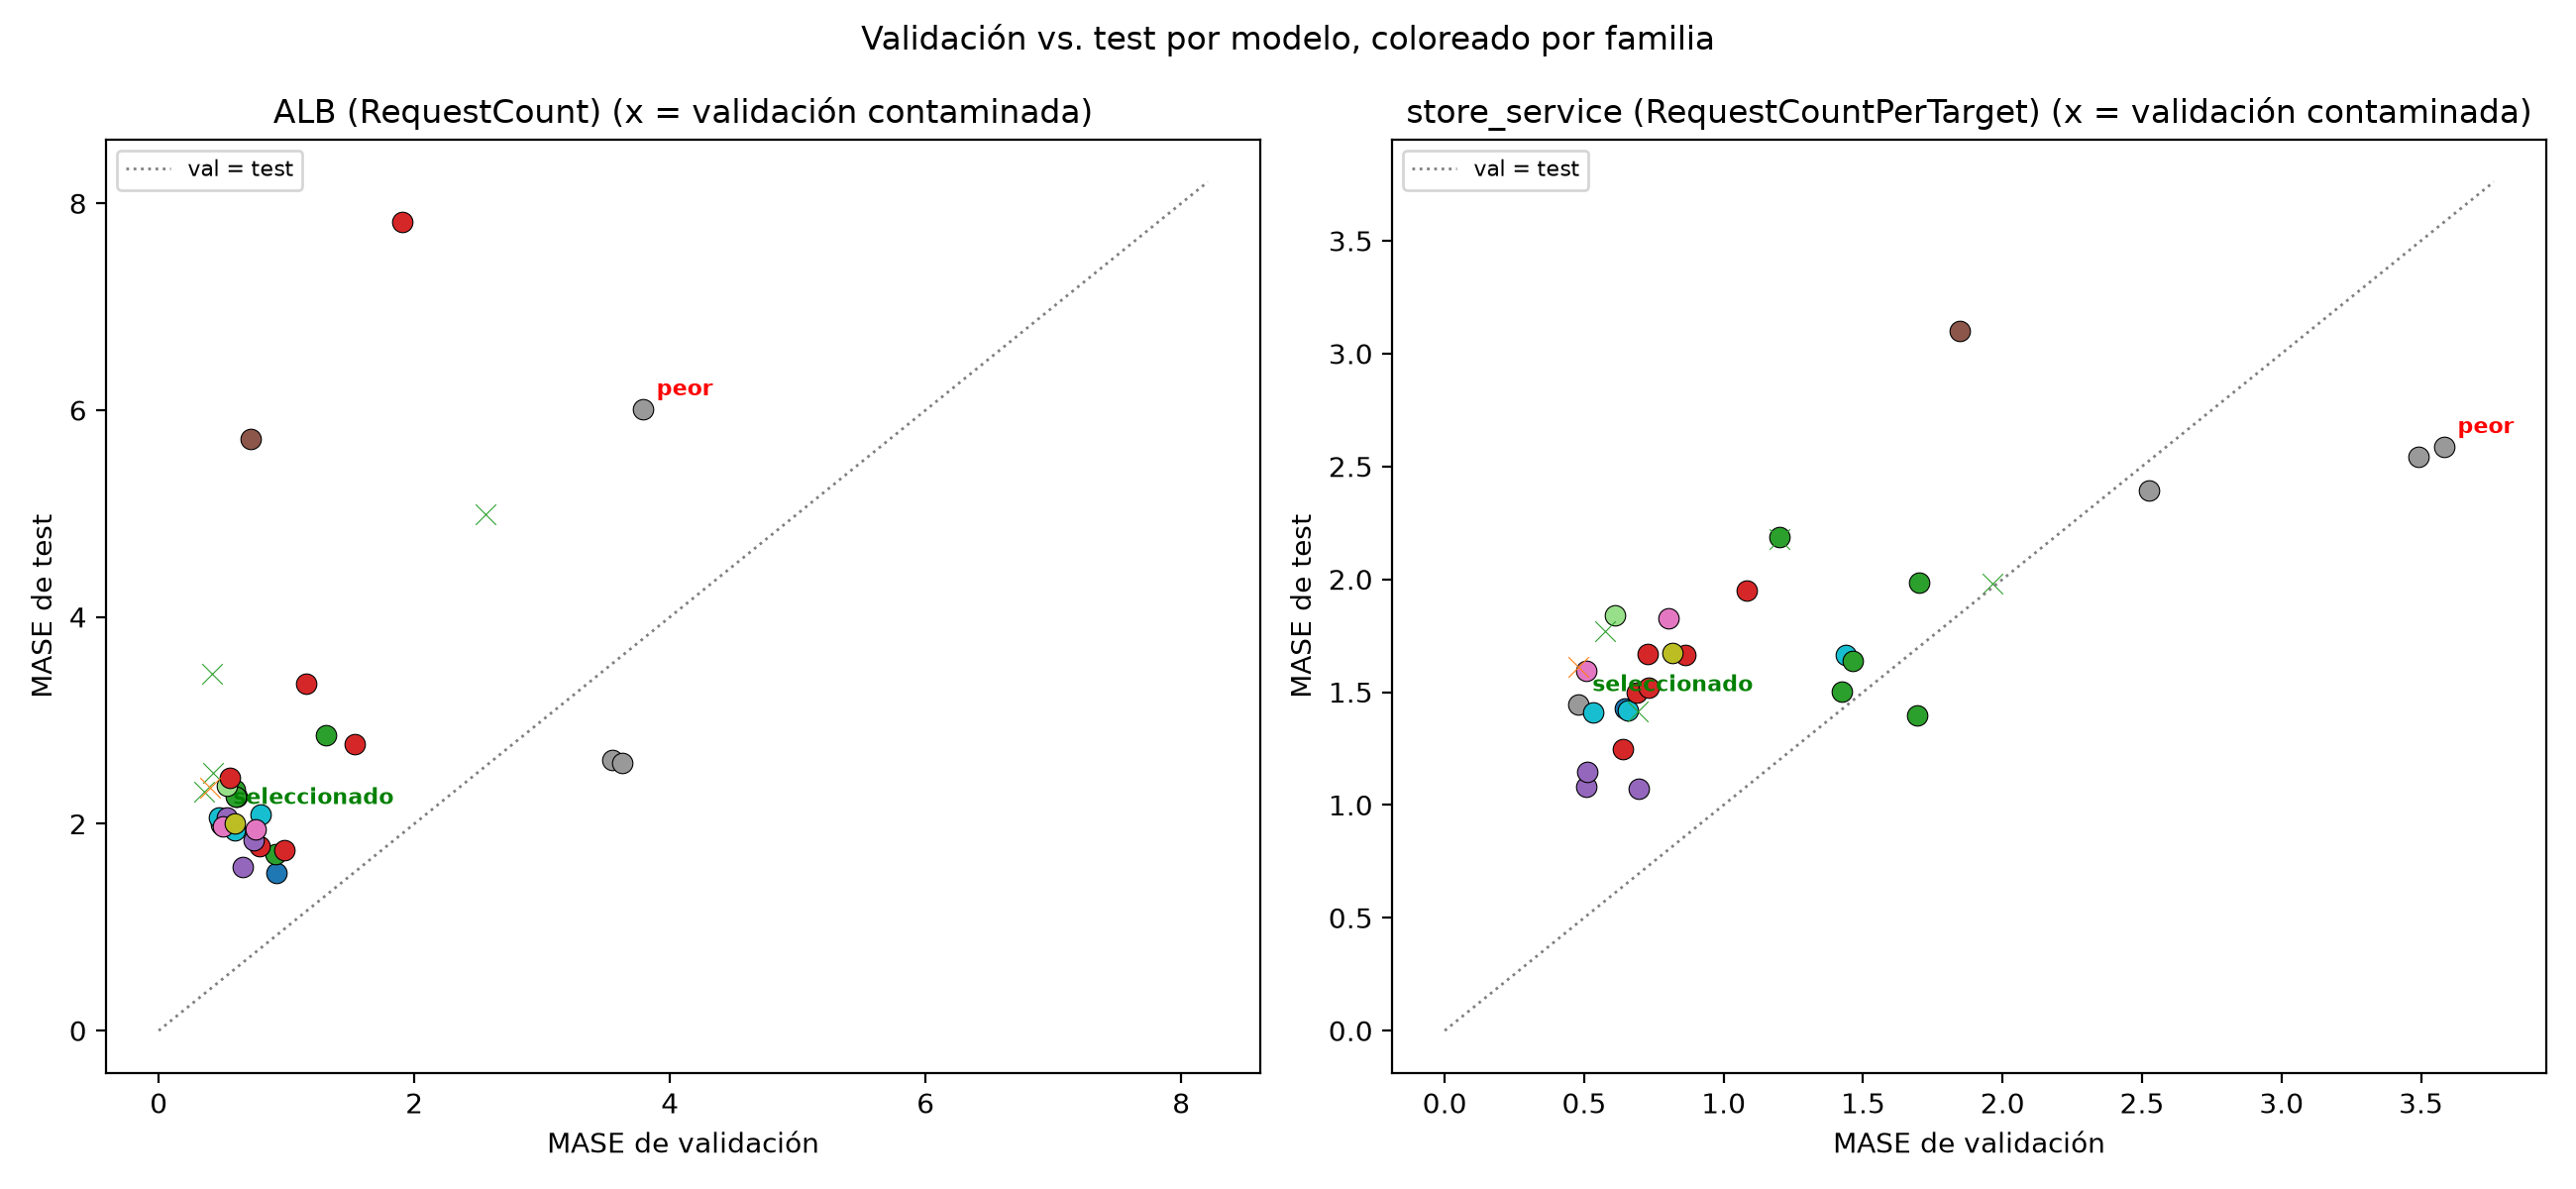
\includegraphics[width=0.85\textwidth]{06_val_vs_test_scatter.png}
  \caption{Dispersión entre el orden de validación y el orden de prueba, ambas series.}
  \label{fig:consistencia}
\end{figure}

La Tabla~\ref{tab:sensibilidad} contrasta la regla adoptada con dos criterios alternativos, a título
exclusivamente informativo: el que se obtendría si se permitieran modelos contaminados, y el que
seleccionaría un oráculo que conociera de antemano el MAE de prueba --un criterio inaplicable en la
práctica, dado que el pronóstico se produce antes de observar el conjunto de prueba--. Cada criterio elige
un ganador distinto en ambas series, lo que evidencia que la elección del criterio de selección no es un
detalle menor del protocolo.

\begin{table}[htbp]
  \centering
  \caption{Análisis de sensibilidad del criterio de selección (no constituye una regla de selección alternativa).}
  \label{tab:sensibilidad}
  \small
  \begin{tabular}{lll}
    \toprule
    Criterio & Serie ALB & Serie store-service \\
    \midrule
    Regla adoptada (MAE val., elegibles) & auto\_arima & seasonal\_naive\_m24 \\
    Incluyendo modelos contaminados & catboost\_tuned & ensemble\_equal\_weight \\
    Oráculo de MAE de prueba\textsuperscript{a} & SARIMA (TP1 refit) & neuralprophet \\
    \bottomrule
  \end{tabular}
  \\[2pt]
  \footnotesize\textsuperscript{a}No utilizable al momento de pronosticar; se incluye solo como referencia
  de contexto.
\end{table}

\subsection{Costo computacional}
\label{sec:costo}

El costo de ajuste no fue el criterio de selección, pero resulta relevante para evaluar la viabilidad
operativa de cada familia. La Tabla~\ref{tab:costo} contrasta los modelos de mayor costo con el modelo
seleccionado. El Transformer de fusión temporal (TFT) exige, por lejos, el mayor tiempo de ajuste del
proyecto (entre 175 y 292 segundos por serie y conjunto, sumado sobre las dos semillas utilizadas), sin
alcanzar el primer puesto en ninguna comparación; AutoGluon TimeSeries exhibe un costo fijo similar,
producto de su límite de tiempo configurado (300 segundos por llamada), independientemente del tamaño de
la serie.

\begin{table}[htbp]
  \centering
  \caption{Tiempo de ajuste de los modelos de mayor costo computacional (segundos).}
  \label{tab:costo}
  \footnotesize
  \begin{tabular}{lp{3.6cm}rr}
    \toprule
    Modelo & Serie & Ajuste (val.) & Reajuste (prueba) \\
    \midrule
    TFT & ALB & 292,41 & 195,67 \\
    TFT & store-service & 271,62 & 175,47 \\
    AutoGluon TimeSeries & ALB & 161,81 & 140,03 \\
    AutoGluon TimeSeries & store-service & 119,65 & 147,21 \\
    auto\_arima & ALB (seleccionado) & 97,52 & 78,93 \\
    auto\_arima & store-service & 79,47 & 46,09 \\
    seasonal\_naive\_m24 & ambas (seleccionado en store-service) & $<0,001$ & $<0,001$ \\
    \bottomrule
  \end{tabular}
\end{table}

\subsection{Pronóstico final a 48 horas}

Con el modelo seleccionado por serie reajustado sobre la totalidad del historial disponible (entrenamiento
más validación, con la intervención imputada), se produce un pronóstico de 48 horas posteriores al final
del historial, entre el 26 de septiembre de 2026 a las 23:00 UTC y el 28 de septiembre de 2026 a las 22:00
UTC. La Figura~\ref{fig:overlay} contrasta, sobre el conjunto de prueba, las trayectorias del modelo
seleccionado, del peor modelo elegible, del SARIMA refit del trabajo anterior y de Chronos, contra el valor
observado; la Figura~\ref{fig:forecast_final} muestra el pronóstico de 48 horas propiamente dicho, con sus
intervalos de predicción.

\begin{figure}[htbp]
  \centering
  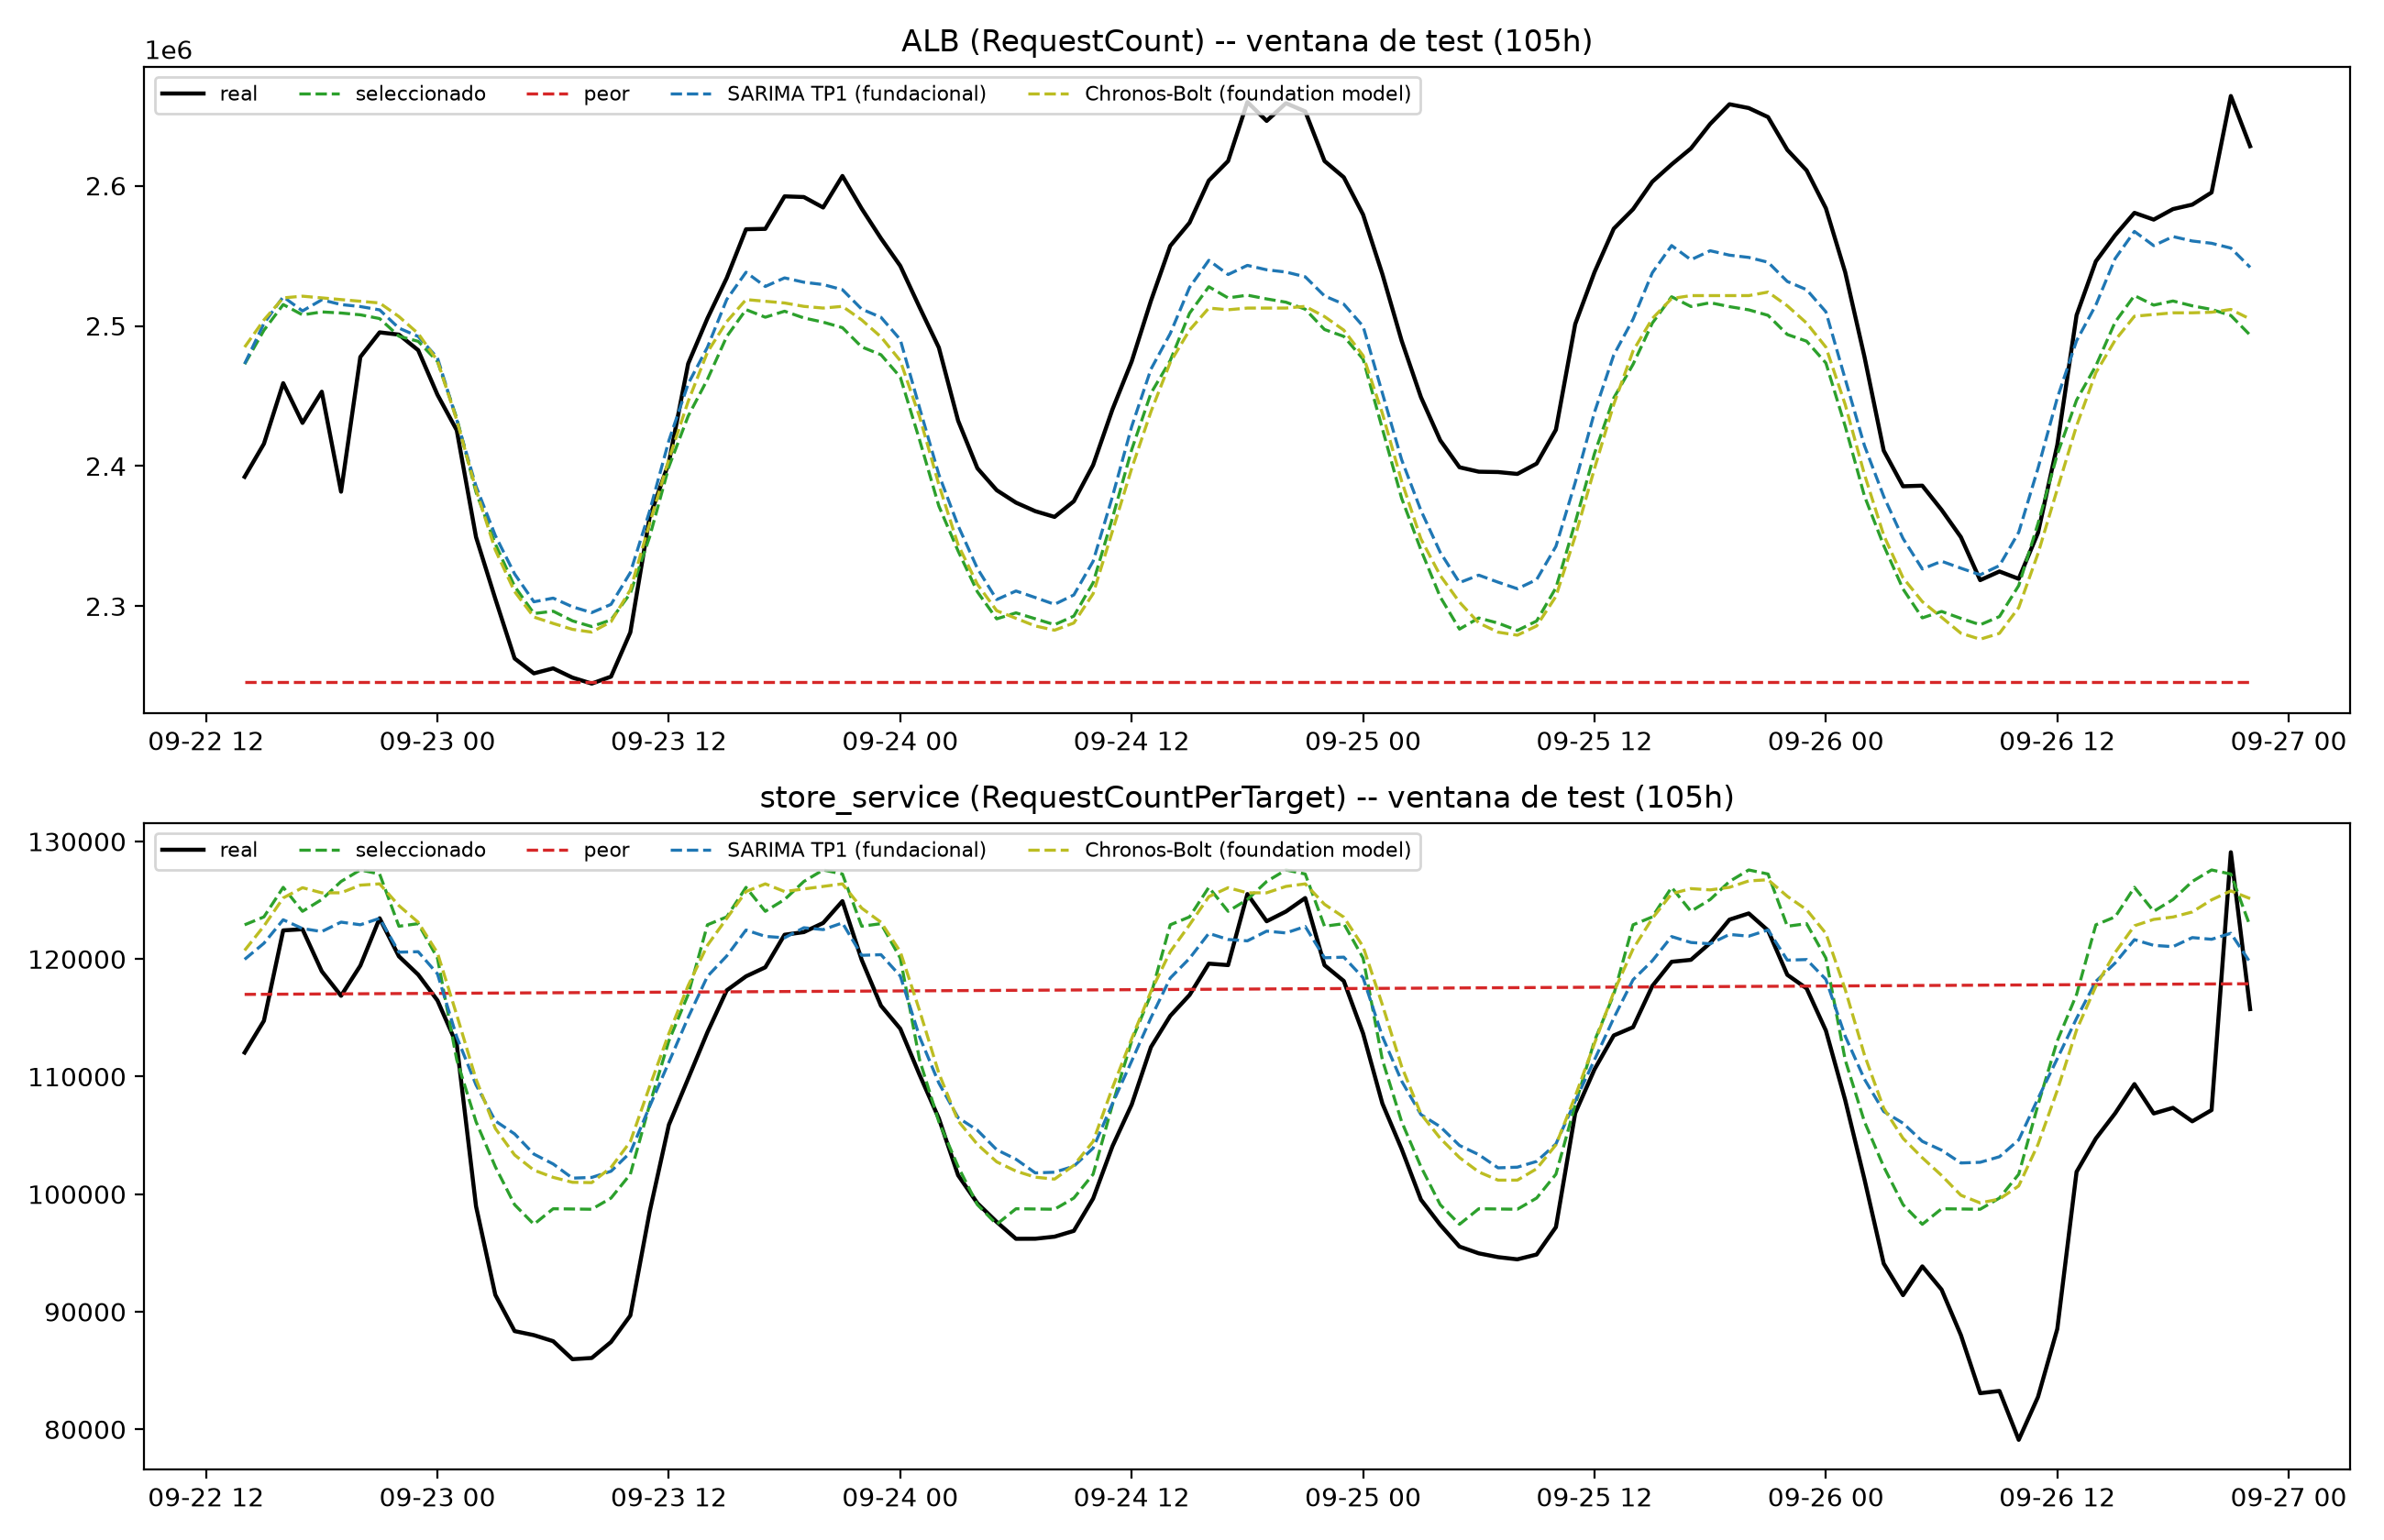
\includegraphics[width=0.92\textwidth]{06_test_overlay_forecast.png}
  \caption{Pronósticos sobre el conjunto de prueba: modelo seleccionado, peor modelo, SARIMA (TP1 refit) y Chronos, ambas series.}
  \label{fig:overlay}
\end{figure}

\begin{figure}[htbp]
  \centering
  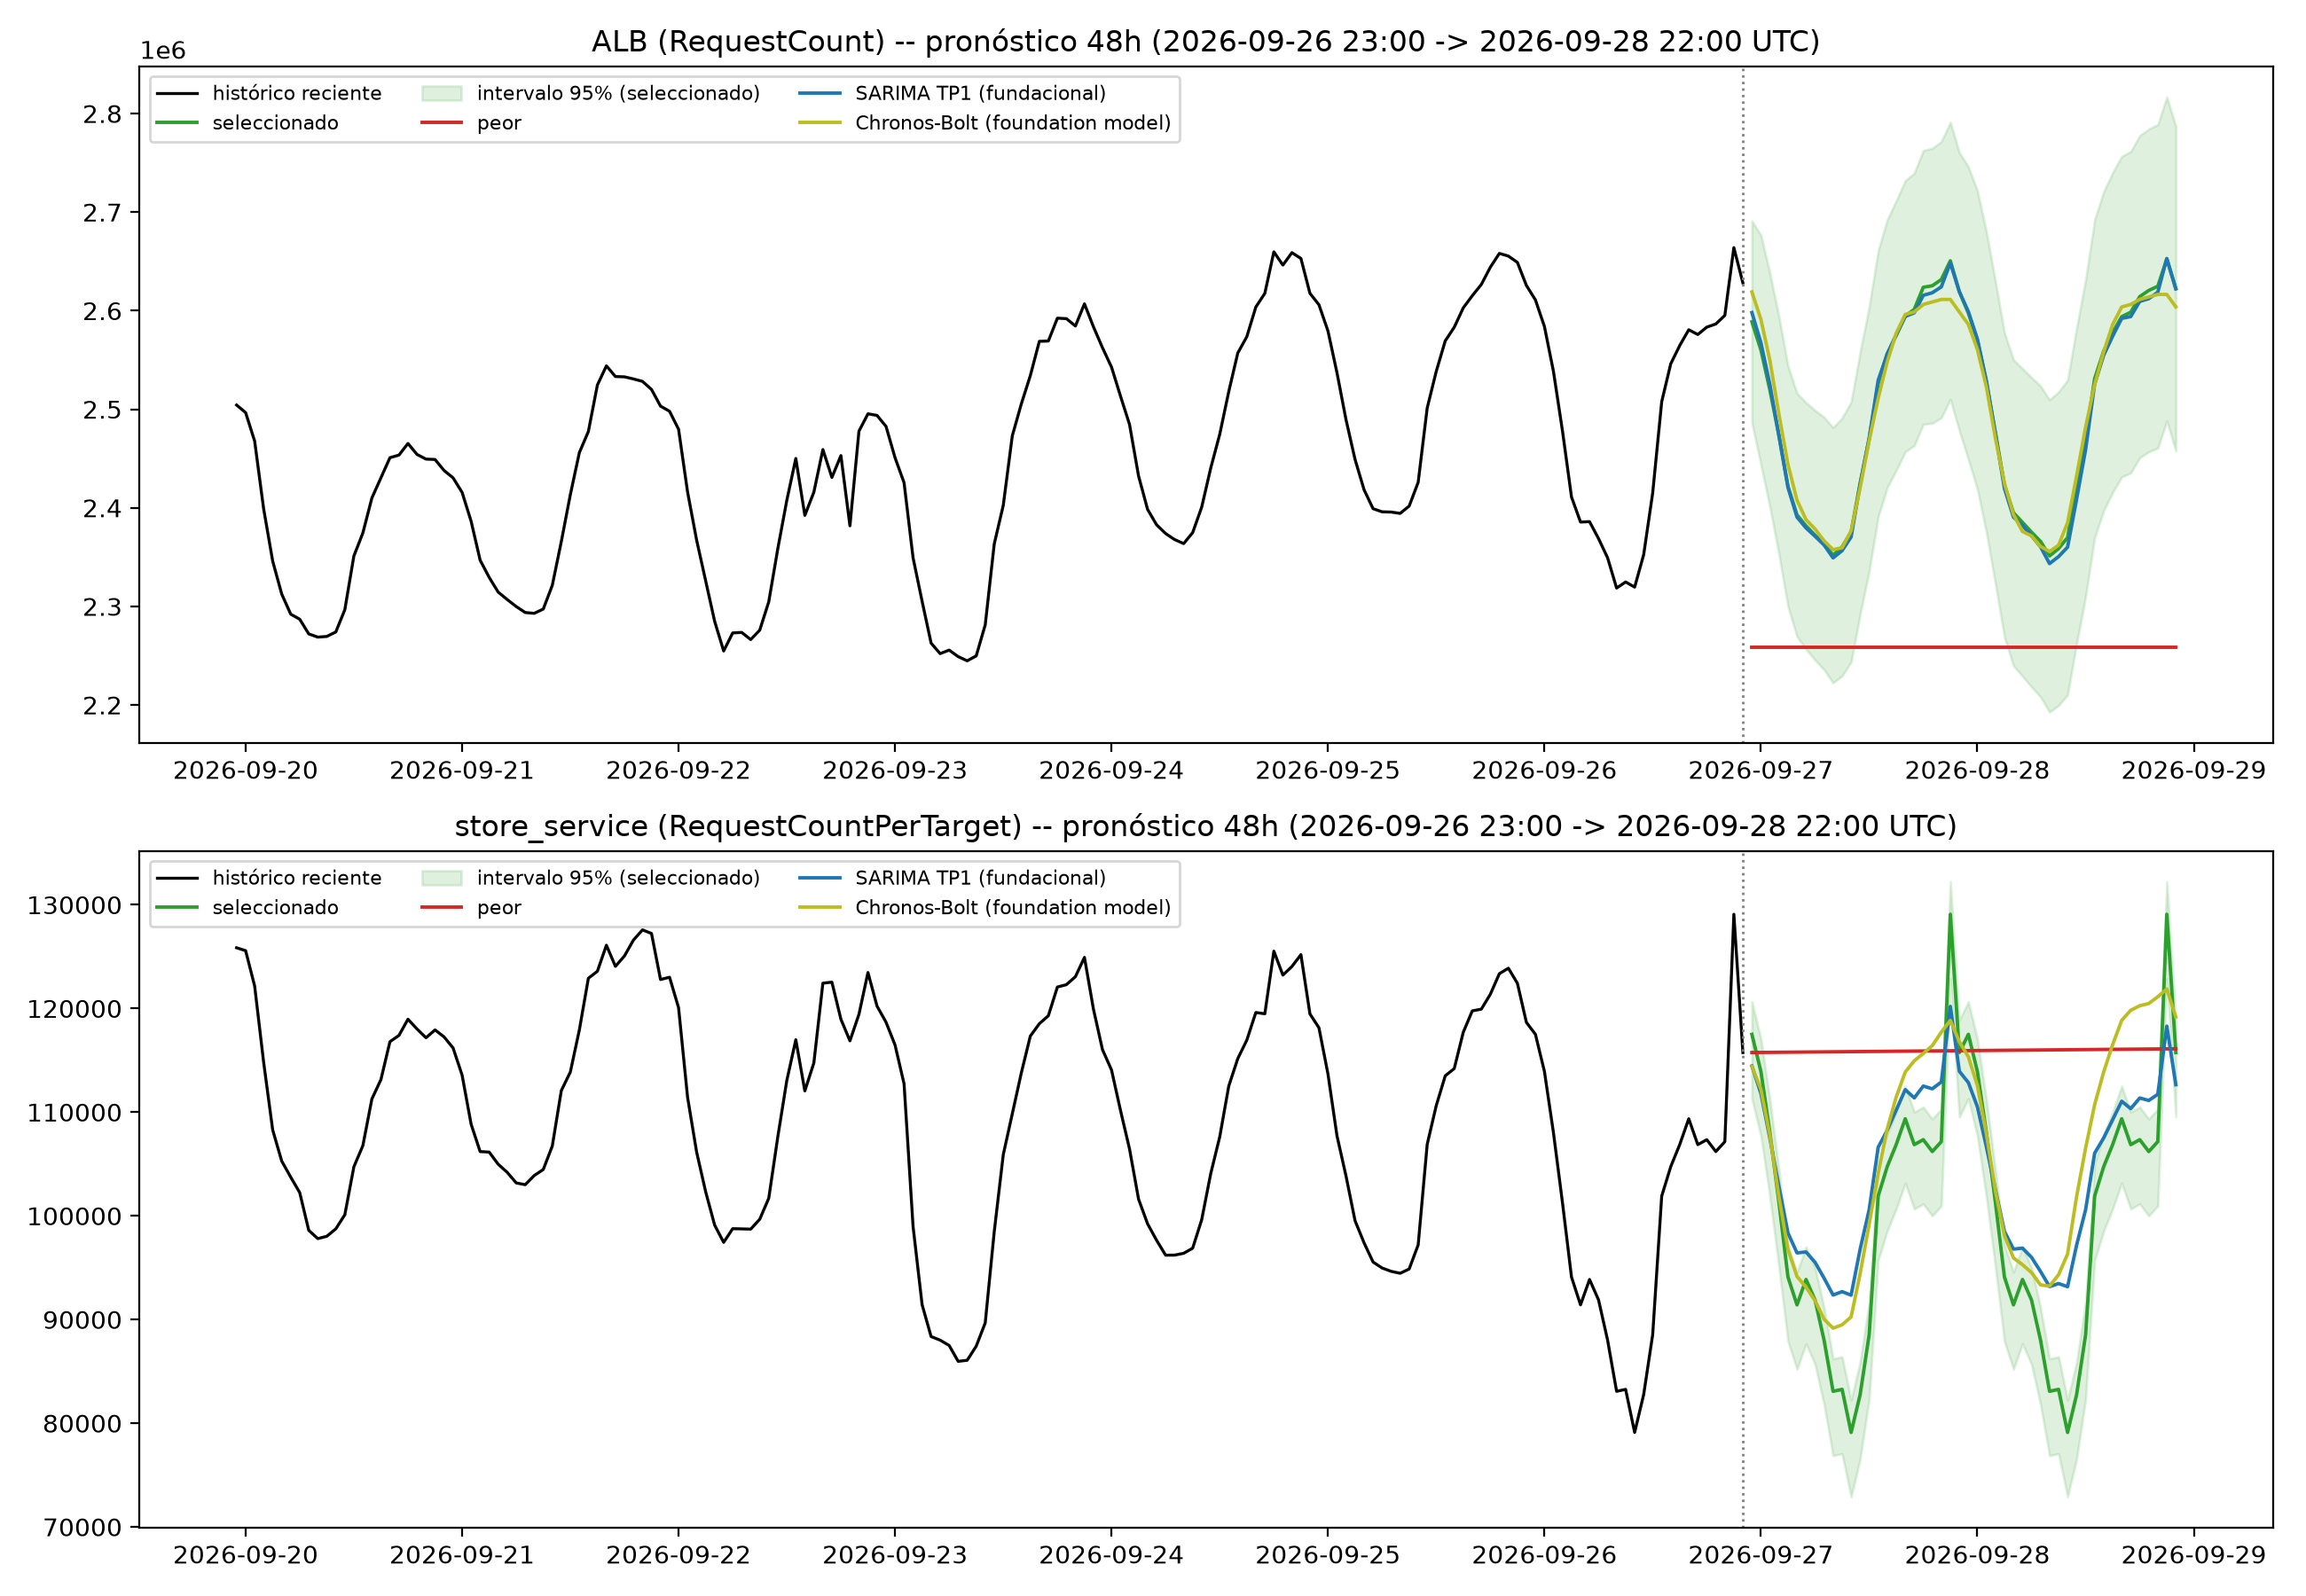
\includegraphics[width=0.92\textwidth]{06_final_forecast.png}
  \caption{Pronóstico final de 48 horas con intervalos de predicción, ambas series.}
  \label{fig:forecast_final}
\end{figure}

Los intervalos de predicción provienen de fuentes distintas según el modelo: AutoARIMA y SARIMA aportan
intervalos nativos de 80\,\% y 95\,\%; la referencia estacional ingenua y el peor modelo elegible utilizan
intervalos empíricos, construidos a partir de los residuos agrupados de la ventana de validación de 48
horas, y por lo tanto constantes en cada hora del horizonte; Chronos aporta únicamente el intervalo del
80\,\%, dado que fue entrenado solo sobre los cuantiles 0,1 y 0,9, y su intervalo del 95\,\% se deja sin
definir en lugar de aproximarse con un cuantil no entrenado.

\pendiente{Serie 3 (a cargo de otro integrante del grupo). Los resultados de esta serie --comparación por
familia de modelos, selección y pronóstico final-- se incorporarán en esta sección una vez completado el
trabajo del integrante responsable.}


% ============ vii. CONCLUSIONES ============
\section{Conclusiones}

\subsection{Síntesis por serie}

El objetivo planteado por la cátedra --determinar si los modelos contemporáneos de Machine Learning, Deep
Learning, modelos híbridos, AutoML y modelos de fundación mejoran el pronóstico obtenido con el enfoque
clásico del Trabajo Práctico N.\textsuperscript{o} 1-- admite una respuesta distinta según la serie y según
el criterio utilizado. Para la serie ALB, el modelo seleccionado mediante la regla honesta de validación
(AutoARIMA) mejora al SARIMA refit en un 48,5\,\% durante la validación, pero resulta un 34,9\,\% peor que
ese mismo SARIMA en el conjunto de prueba; de las 32 configuraciones evaluadas, el propio SARIMA refit del
trabajo anterior es, en definitiva, la de mejor desempeño de prueba. En esta serie, entonces, el enfoque
clásico del trabajo anterior no fue superado por ningún modelo más reciente cuando se lo evalúa sobre datos
no vistos durante el ajuste. Para la serie store-service, el modelo seleccionado (la referencia estacional
ingenua) tampoco es superado en validación por ningún modelo no contaminado, pero en el conjunto de prueba
sí lo supera un modelo de la familia Prophet (NeuralProphet, un 25,8\,\% mejor MASE que el modelo
seleccionado), aunque ese modelo no habría sido elegido por la regla honesta de selección, dado su
desempeño mediocre en validación (decimocuarto puesto de 32). La respuesta general, entonces, es matizada:
los modelos más recientes pueden superar al enfoque clásico, pero no necesariamente lo hacen los mismos
modelos que una regla de selección basada exclusivamente en validación elegiría.

\subsection{Consistencia entre validación y prueba}

La correlación de Spearman entre el orden de validación y el de prueba resultó baja y no significativa
para ALB ($\rho=0,237$, $p=0,192$ sobre las 32 configuraciones) y moderada y significativa para
store-service ($\rho=0,654$, $p<0,001$). Esta diferencia entre series sugiere que la propia confiabilidad
del protocolo de validación --y, por lo tanto, la confianza que puede depositarse en el modelo
seleccionado-- no es uniforme: para ALB, una ventana de validación de 48 horas ordena a los modelos de un
modo que guarda poca relación con su desempeño posterior, mientras que para store-service ese orden es más
informativo, aunque tampoco infalible, como lo demuestra el caso de NeuralProphet.

\subsection{Serie pública de contraste}

Sobre la serie de visitas horarias a Wikipedia en español, con seis modelos de hiperparámetros por defecto,
la regla de selección por validación eligió la referencia estacional ingenua, mientras que en prueba el mejor
modelo fue Ridge y el SARIMA del trabajo anterior el peor (2,513). El resultado es
coherente con la conclusión general del trabajo: el desempeño relativo del enfoque clásico depende de la
serie (fue el mejor en ALB y el peor en Wikipedia), y el orden de validación no anticipa el de prueba (Spearman
de 0,09 sobre seis modelos). Por su alcance reducido, este resultado se interpreta como un contraste y no
como una evaluación completa.

\subsection{Límites del trabajo}

\begin{enumerate}
  \item \textbf{Ventana única de validación.} El protocolo utiliza una sola ventana de contraste de 48
  horas, en lugar de una validación cruzada expandida de múltiples pliegues, debido al tiempo de cómputo
  que exige comparar 32 configuraciones por serie. Esta decisión probablemente explica, al menos en parte,
  la baja consistencia entre validación y prueba observada en ALB: una sola ventana de 48 horas es una
  muestra pequeña del comportamiento futuro de la serie y su resultado puede estar dominado por
  particularidades de esas horas específicas.
  \item \textbf{Historial todavía acotado.} El historial efectivo disponible cubre 86 días (2.063
  observaciones horarias), sensiblemente más que el mes del trabajo anterior, pero aún reducido para
  arquitecturas de Deep Learning con una cantidad considerable de parámetros, que pueden requerir un
  historial más extenso para generalizar de forma estable.
  \item \textbf{Modelos con puntaje de validación contaminado.} Cinco de las 32 configuraciones por serie
  utilizan, para su propio ajuste de hiperparámetros o para la elección de sus miembros, la misma ventana
  de 48 horas luego utilizada para clasificarlas. Estos modelos se documentan y se muestran en las tablas y
  figuras de este informe, pero se excluyen de la selección; de haberse permitido, la regla habría
  seleccionado un modelo distinto en ambas series (Tabla~\ref{tab:sensibilidad}), sin que ello implicara una
  mejora real en el conjunto de prueba.
  \item \textbf{Posible anomalía en las últimas horas de store-service.} Las últimas horas registradas de
  la serie store-service (20:00 a 22:00 UTC del 26 de septiembre de 2026) muestran un patrón que se aparta
  del comportamiento de esas mismas horas en los cuatro días anteriores: una caída inusual a las 20:00 UTC,
  seguida de un valor por encima de lo esperado a las 21:00 UTC. No se identificó un patrón equivalente en
  la serie ALB durante esas mismas horas. Esta observación no fue investigada en profundidad y no se
  descarta que corresponda a un artefacto puntual de exportación de datos más que a un cambio real del
  proceso subyacente; se documenta aquí como una limitación abierta y no como un hallazgo verificado.
  \item \textbf{Estacionalidad semanal no aprovechada.} La estacionalidad semanal, débil pero no nula
  (fuerza de 0,206 en ALB y 0,311 en store-service según la descomposición MSTL), se excluyó de los modelos
  Prophet y NeuralProphet y del período estacional del MASE, sobre la base de un historial que, con 86
  días, apenas cubre unas doce semanas completas; un historial más extenso podría justificar su
  incorporación.
  \item \textbf{Serie pública con alcance acotado.} La serie de Wikipedia se evaluó con seis modelos de
  hiperparámetros por defecto, sin Deep Learning, AutoML ni modelos de fundación, con una única ventana de
  validación de 48 horas y una de prueba de 105 horas, y con un SARIMA cuya especificación proviene de ALB.
  Ridge y LightGBM reciben como variable exógena la marca de intervención del despliegue, que vale 1 entre el 17 y el 22 de septiembre aunque esta serie no fue afectada; con la marca en cero, el MASE de prueba de Ridge pasa de 0,784 a 0,756 y el de LightGBM no cambia, sin alterar el orden de los modelos ni el de validación.
  Sus resultados no son comparables uno a uno con los de las 32 configuraciones de las series de BodegaAI.
\end{enumerate}

\subsection{Líneas de trabajo futuro}

La continuación más directa de este trabajo consiste en reemplazar la ventana única de validación por un
esquema de validación cruzada de múltiples orígenes (\emph{multi-origin validation}), en la línea de lo
propuesto por \textcite{hyndman2021}, que estime el error de generalización sobre varias ventanas
sucesivas en lugar de una sola. Una segunda línea consiste en extender el historial disponible una vez que
transcurra más tiempo desde la puesta en producción del sistema, lo que permitiría evaluar con mayor
solidez tanto la estacionalidad semanal como la estabilidad de las arquitecturas de Deep Learning de mayor
capacidad. Finalmente, la serie pública de Wikipedia se trató aquí solo como una línea base acotada; extenderle la
batería completa (Deep Learning, AutoML, modelos de fundación y búsqueda de hiperparámetros) permitiría
contrastar con mayor solidez si las conclusiones alcanzadas para las dos series de infraestructura de
BodegaAI se sostienen en un dominio de datos distinto.




% ============ Declaración de uso de IA generativa ============
\newpage
\section*{Declaración de uso de IA generativa}
\addcontentsline{toc}{section}{Declaración de uso de IA generativa}

Siguiendo las recomendaciones de transparencia para citar y describir el uso de IA generativa
en trabajos académicos \parencite{mcadoo2025generativeai}, se declara que durante el desarrollo
de este trabajo se emplearon agentes de IA generativa (Claude Code, de Anthropic, con el
modelo Sonnet) como apoyo para la exploración del repositorio, el desarrollo y la revisión del
código, y la redacción y edición del presente informe \parencite{anthropic2026claude_code_sonnet}.
El uso de estas herramientas tuvo carácter asistivo: las decisiones metodológicas, la selección
de datos, la ejecución de los análisis, la validación de resultados y la responsabilidad final
del informe corresponden a los autores.

% ============ viii. REFERENCIAS BIBLIOGRÁFICAS ============
\newpage
\printbibliography[title={Referencias bibliográficas}, heading=bibintoc]

% ============ ix. APÉNDICES ============
\appendix

\section{Apéndice A. Tablas completas y material gráfico complementario}

Las figuras y tablas de este apéndice documentan el análisis exploratorio y el conjunto completo de 32
configuraciones evaluadas por serie. Se excluyeron del cuerpo del informe por resultar redundantes
respecto de las figuras allí incluidas, por referir a aspectos discutidos únicamente de forma numérica en
el cuerpo, o por exceder el detalle necesario para sostener sus afirmaciones centrales.

\begingroup
\tiny
\begin{longtable}{llrrrrc}
  \caption{Conjunto completo de 32 configuraciones evaluadas -- serie ALB.}
  \label{tab:completo_alb}\\
  \toprule
  Modelo & Familia & MAE val. & MASE val. & MAE prueba & MASE prueba & Contam. \\
  \midrule
  \endfirsthead
  \multicolumn{7}{l}{\small \tablename\ \thetable{} (continuación)}\\
  \toprule
  Modelo & Familia & MAE val. & MASE val. & MAE prueba & MASE prueba & Contam. \\
  \midrule
  \endhead
  \bottomrule
  \endfoot
    naive & Ingenuo & 140.474,23 & 3,548 & 103.514,69 & 2,615 & No \\
    seasonal\_naive\_m24 & Ingenuo & 19.369,02 & 0,489 & 78.784,34 & 1,990 & No \\
    drift & Ingenuo & 143.670,97 & 3,629 & 102.288,71 & 2,584 & No \\
    average & Ingenuo & 149.950,95 & 3,788 & 237.950,60 & 6,011 & No \\
    SARIMA (TP1 refit) & Fundacional TP1 & 36.524,57 & 0,923 & 60.429,07 & 1,526 & No \\
    holt\_winters & Clásico & 31.604,81 & 0,798 & 82.913,56 & 2,094 & No \\
    mstl\_arima & Clásico & 23.468,84 & 0,593 & 76.674,57 & 1,937 & No \\
    auto\_arima & Clásico & 18.807,50 & 0,475 & 81.488,75 & 2,058 & No \\
    lightgbm & ML & 24.100,55 & 0,609 & 89.523,11 & 2,261 & No \\
    xgboost & ML & 51.766,94 & 1,308 & 113.131,51 & 2,858 & No \\
    catboost & ML & 23.676,28 & 0,598 & 92.090,22 & 2,326 & No \\
    random\_forest & ML & 24.013,59 & 0,607 & 89.523,51 & 2,261 & No \\
    ridge & ML & 36.145,98 & 0,913 & 67.461,63 & 1,704 & No \\
    catboost\_direct & ML (directo) & 21.126,48 & 0,534 & 93.581,28 & 2,364 & No \\
    catboost\_tuned & ML & 13.994,36 & 0,353 & 91.577,78 & 2,313 & Sí \\
    random\_forest\_tuned & ML & 16.478,21 & 0,416 & 136.787,15 & 3,455 & Sí \\
    lightgbm\_tuned & ML & 16.682,37 & 0,421 & 98.698,42 & 2,493 & Sí \\
    stacking\_top3 & ML & 101.301,74 & 2,559 & 197.519,54 & 4,989 & Sí \\
    lstm & DL & 75.584,94 & 1,909 & 309.470,41 & 7,817 & No \\
    nbeats & DL & 38.805,46 & 0,980 & 69.030,03 & 1,744 & No \\
    nhits & DL & 22.021,71 & 0,556 & 96.620,17 & 2,441 & No \\
    tcn & DL & 45.631,83 & 1,153 & 132.828,03 & 3,355 & No \\
    tft & DL & 60.751,26 & 1,535 & 109.629,69 & 2,769 & No \\
    tide & DL & 31.271,07 & 0,790 & 70.489,78 & 1,781 & No \\
    prophet\_default & Prophet & 21.066,96 & 0,532 & 81.749,90 & 2,065 & No \\
    prophet\_tuned & Prophet & 26.085,28 & 0,659 & 62.468,36 & 1,578 & No \\
    neuralprophet & Prophet & 29.444,69 & 0,744 & 72.996,75 & 1,844 & No \\
    mstl\_lightgbm & Híbrido & 28.341,14 & 0,716 & 226.471,23 & 5,721 & No \\
    autogluon\_timeseries & AutoML & 19.748,53 & 0,499 & 78.152,68 & 1,974 & No \\
    autots & AutoML & 29.913,83 & 0,756 & 77.200,09 & 1,950 & No \\
    chronos\_bolt\_base & Fundación & 23.678,74 & 0,598 & 79.453,52 & 2,007 & No \\
    ensemble\_equal\_weight & Ensamble & 16.006,29 & 0,404 & 93.116,04 & 2,352 & Sí \\
\end{longtable}
\endgroup

\begingroup
\tiny
\begin{longtable}{llrrrrc}
  \caption{Conjunto completo de 32 configuraciones evaluadas -- serie store-service.}
  \label{tab:completo_store}\\
  \toprule
  Modelo & Familia & MAE val. & MASE val. & MAE prueba & MASE prueba & Contam. \\
  \midrule
  \endfirsthead
  \multicolumn{7}{l}{\small \tablename\ \thetable{} (continuación)}\\
  \toprule
  Modelo & Familia & MAE val. & MASE val. & MAE prueba & MASE prueba & Contam. \\
  \midrule
  \endhead
  \bottomrule
  \endfoot
    naive & Ingenuo & 16.585,83 & 3,490 & 12.080,82 & 2,542 & No \\
    seasonal\_naive\_m24 & Ingenuo & 2.281,85 & 0,480 & 6.858,35 & 1,443 & No \\
    drift & Ingenuo & 17.022,66 & 3,582 & 12.292,99 & 2,587 & No \\
    average & Ingenuo & 11.991,26 & 2,523 & 11.365,28 & 2,392 & No \\
    SARIMA (TP1 refit) & Fundacional TP1 & 3.075,43 & 0,647 & 6.775,50 & 1,426 & No \\
    holt\_winters & Clásico & 6.840,69 & 1,439 & 7.910,62 & 1,665 & No \\
    mstl\_arima & Clásico & 3.116,58 & 0,656 & 6.738,21 & 1,418 & No \\
    auto\_arima & Clásico & 2.525,88 & 0,532 & 6.693,19 & 1,408 & No \\
    lightgbm & ML & 6.763,12 & 1,423 & 7.134,86 & 1,501 & No \\
    xgboost & ML & 6.958,01 & 1,464 & 7.781,26 & 1,637 & No \\
    catboost & ML & 8.076,39 & 1,700 & 9.427,28 & 1,984 & No \\
    random\_forest & ML & 8.057,11 & 1,695 & 6.644,16 & 1,398 & No \\
    ridge & ML & 5.709,70 & 1,201 & 10.402,06 & 2,189 & No \\
    ridge\_direct & ML (directo) & 2.905,15 & 0,611 & 8.742,22 & 1,840 & No \\
    ridge\_tuned & ML & 5.707,42 & 1,201 & 10.342,18 & 2,176 & Sí \\
    lightgbm\_tuned & ML & 2.723,67 & 0,573 & 8.411,54 & 1,770 & Sí \\
    xgboost\_tuned & ML & 3.281,09 & 0,690 & 6.723,50 & 1,415 & Sí \\
    stacking\_top3 & ML & 9.327,31 & 1,963 & 9.412,96 & 1,981 & Sí \\
    lstm & DL & 3.458,53 & 0,728 & 7.928,91 & 1,668 & No \\
    nbeats & DL & 3.031,39 & 0,638 & 5.927,84 & 1,247 & No \\
    nhits & DL & 3.276,37 & 0,689 & 7.119,14 & 1,498 & No \\
    tcn & DL & 3.476,89 & 0,732 & 7.223,69 & 1,520 & No \\
    tft & DL & 5.147,35 & 1,083 & 9.260,54 & 1,949 & No \\
    tide & DL & 4.094,99 & 0,862 & 7.909,85 & 1,664 & No \\
    prophet\_default & Prophet & 2.405,88 & 0,506 & 5.145,67 & 1,083 & No \\
    prophet\_tuned & Prophet & 2.432,33 & 0,512 & 5.439,47 & 1,145 & No \\
    neuralprophet & Prophet & 3.297,54 & 0,694 & 5.090,39 & 1,071 & No \\
    mstl\_lightgbm & Híbrido & 8.779,73 & 1,848 & 14.729,52 & 3,100 & No \\
    autogluon\_timeseries & AutoML & 3.808,36 & 0,801 & 8.677,17 & 1,826 & No \\
    autots & AutoML & 2.412,97 & 0,508 & 7.582,50 & 1,596 & No \\
    chronos\_bolt\_base & Fundación & 3.877,73 & 0,816 & 7.949,65 & 1,673 & No \\
    ensemble\_equal\_weight & Ensamble & 2.281,64 & 0,480 & 7.661,02 & 1,612 & Sí \\
\end{longtable}
\endgroup

\begin{figure}[htbp]
  \centering
  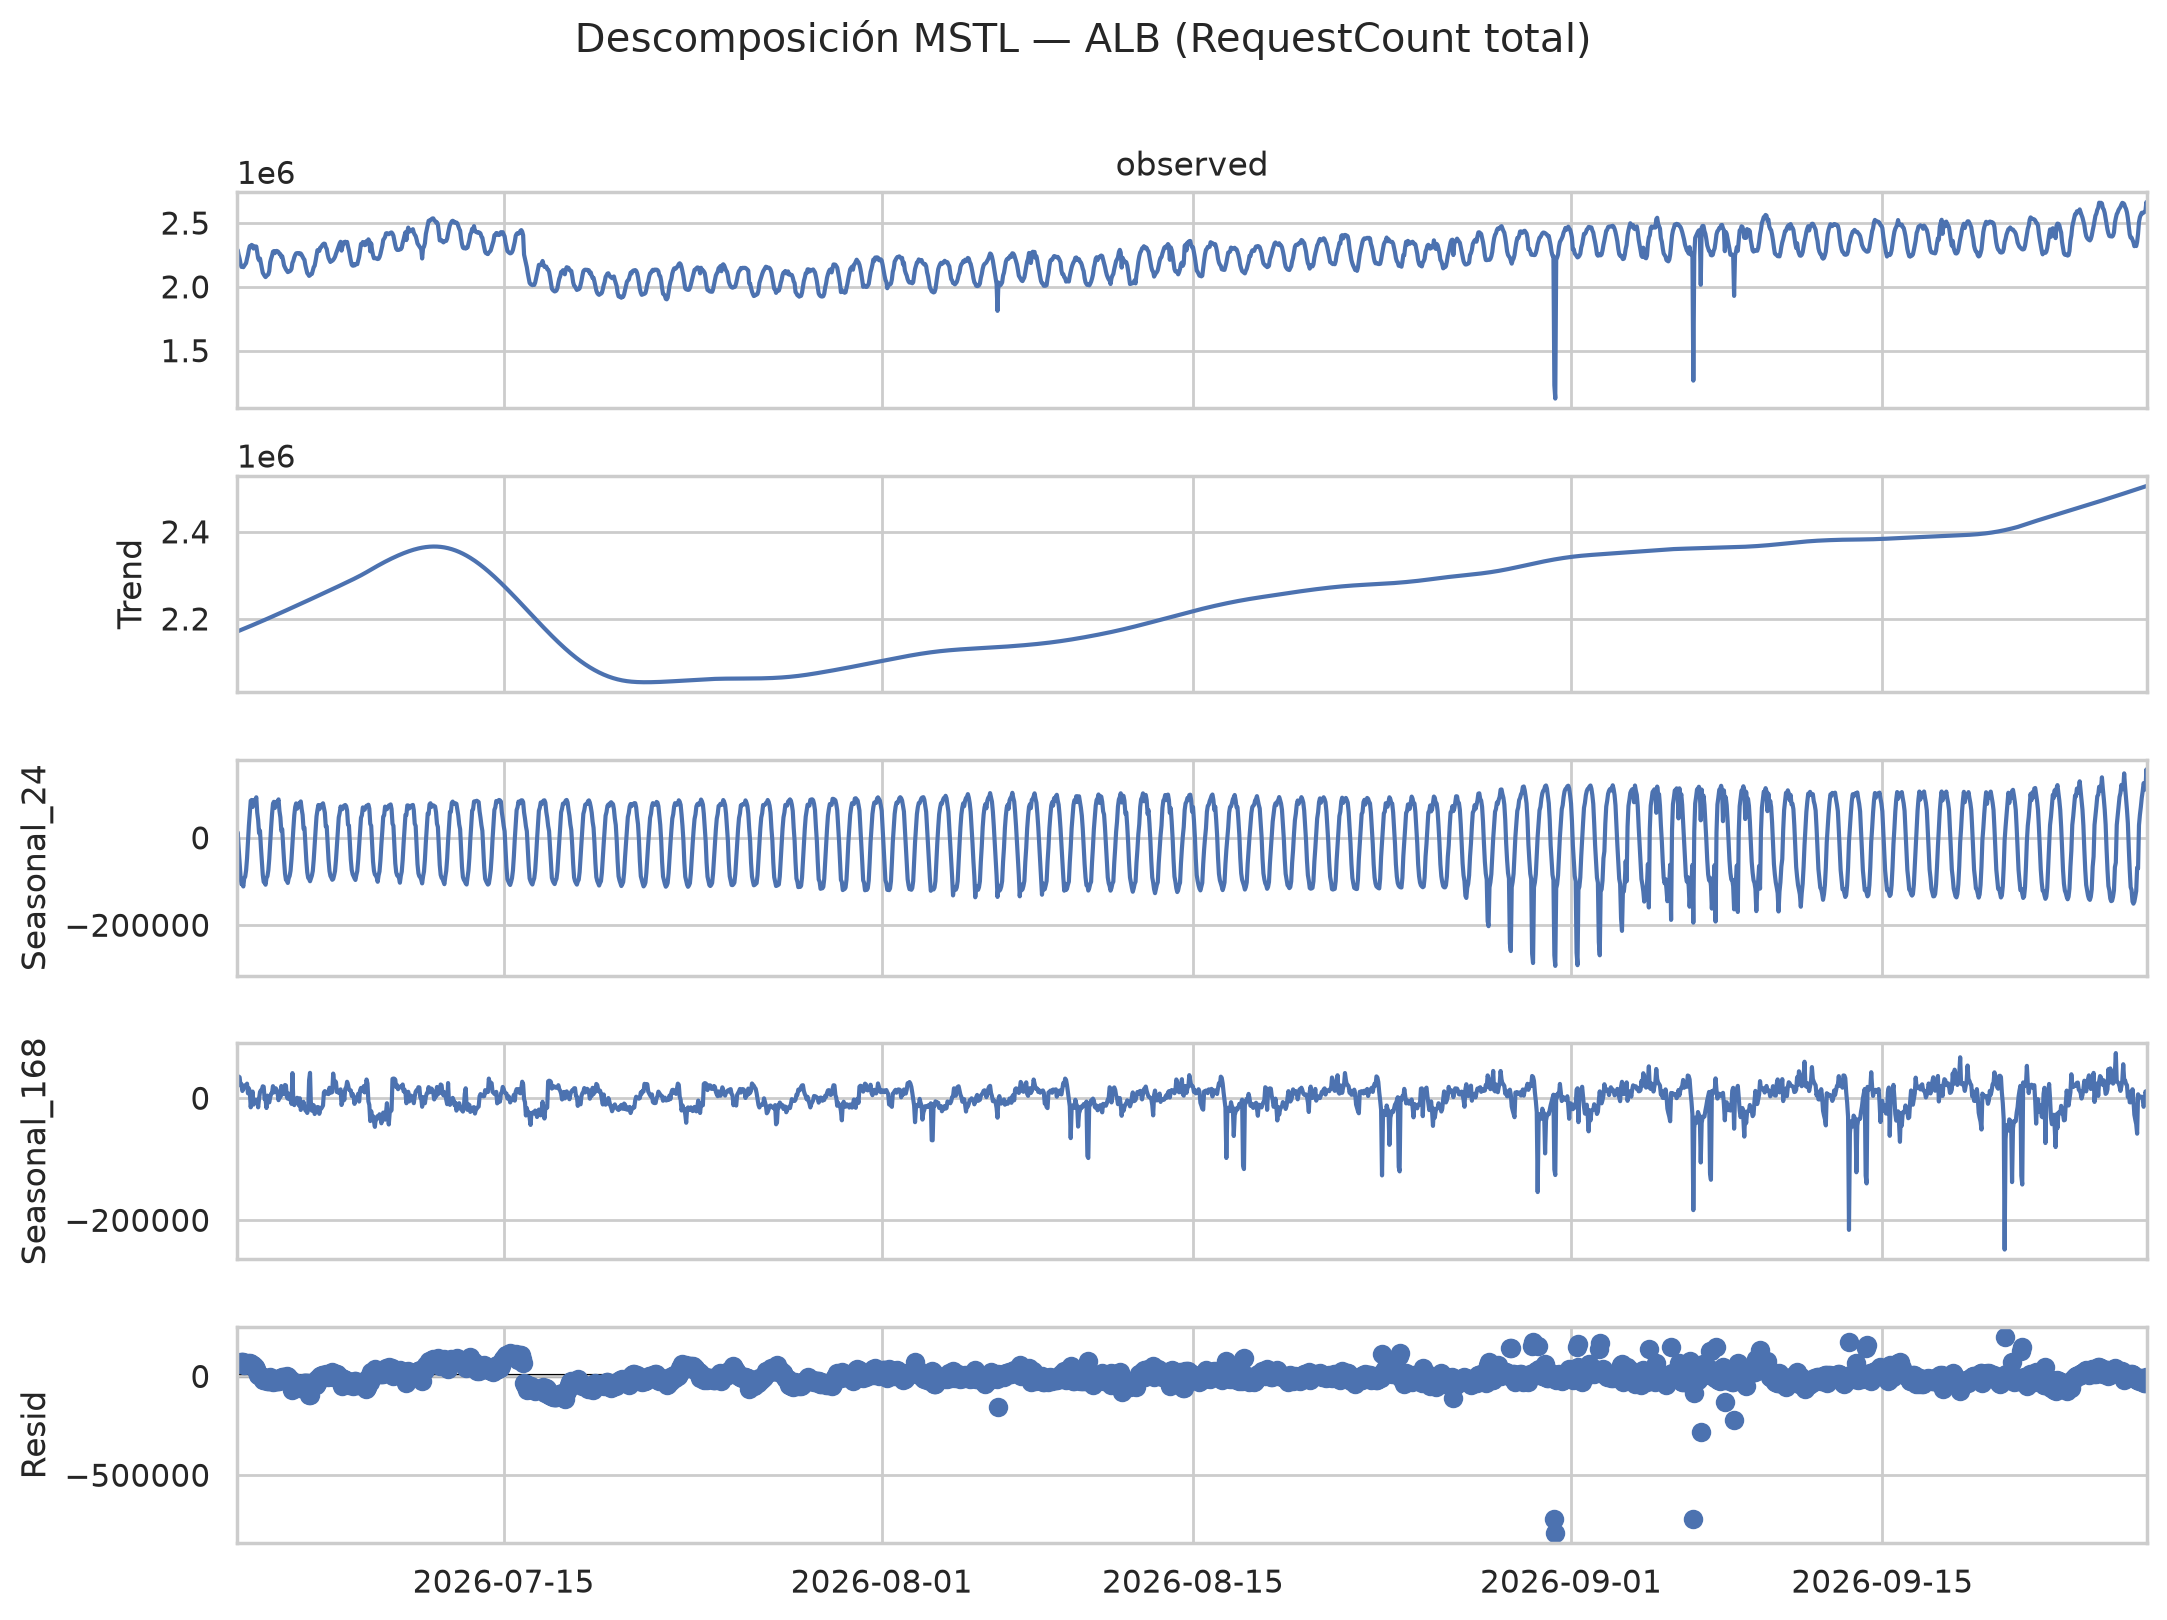
\includegraphics[width=0.85\textwidth]{01_mstl_alb.png}
  \caption{Descomposición MSTL (tendencia, estacionalidad diaria y semanal, residuo), serie ALB.}
\end{figure}

\begin{figure}[htbp]
  \centering
  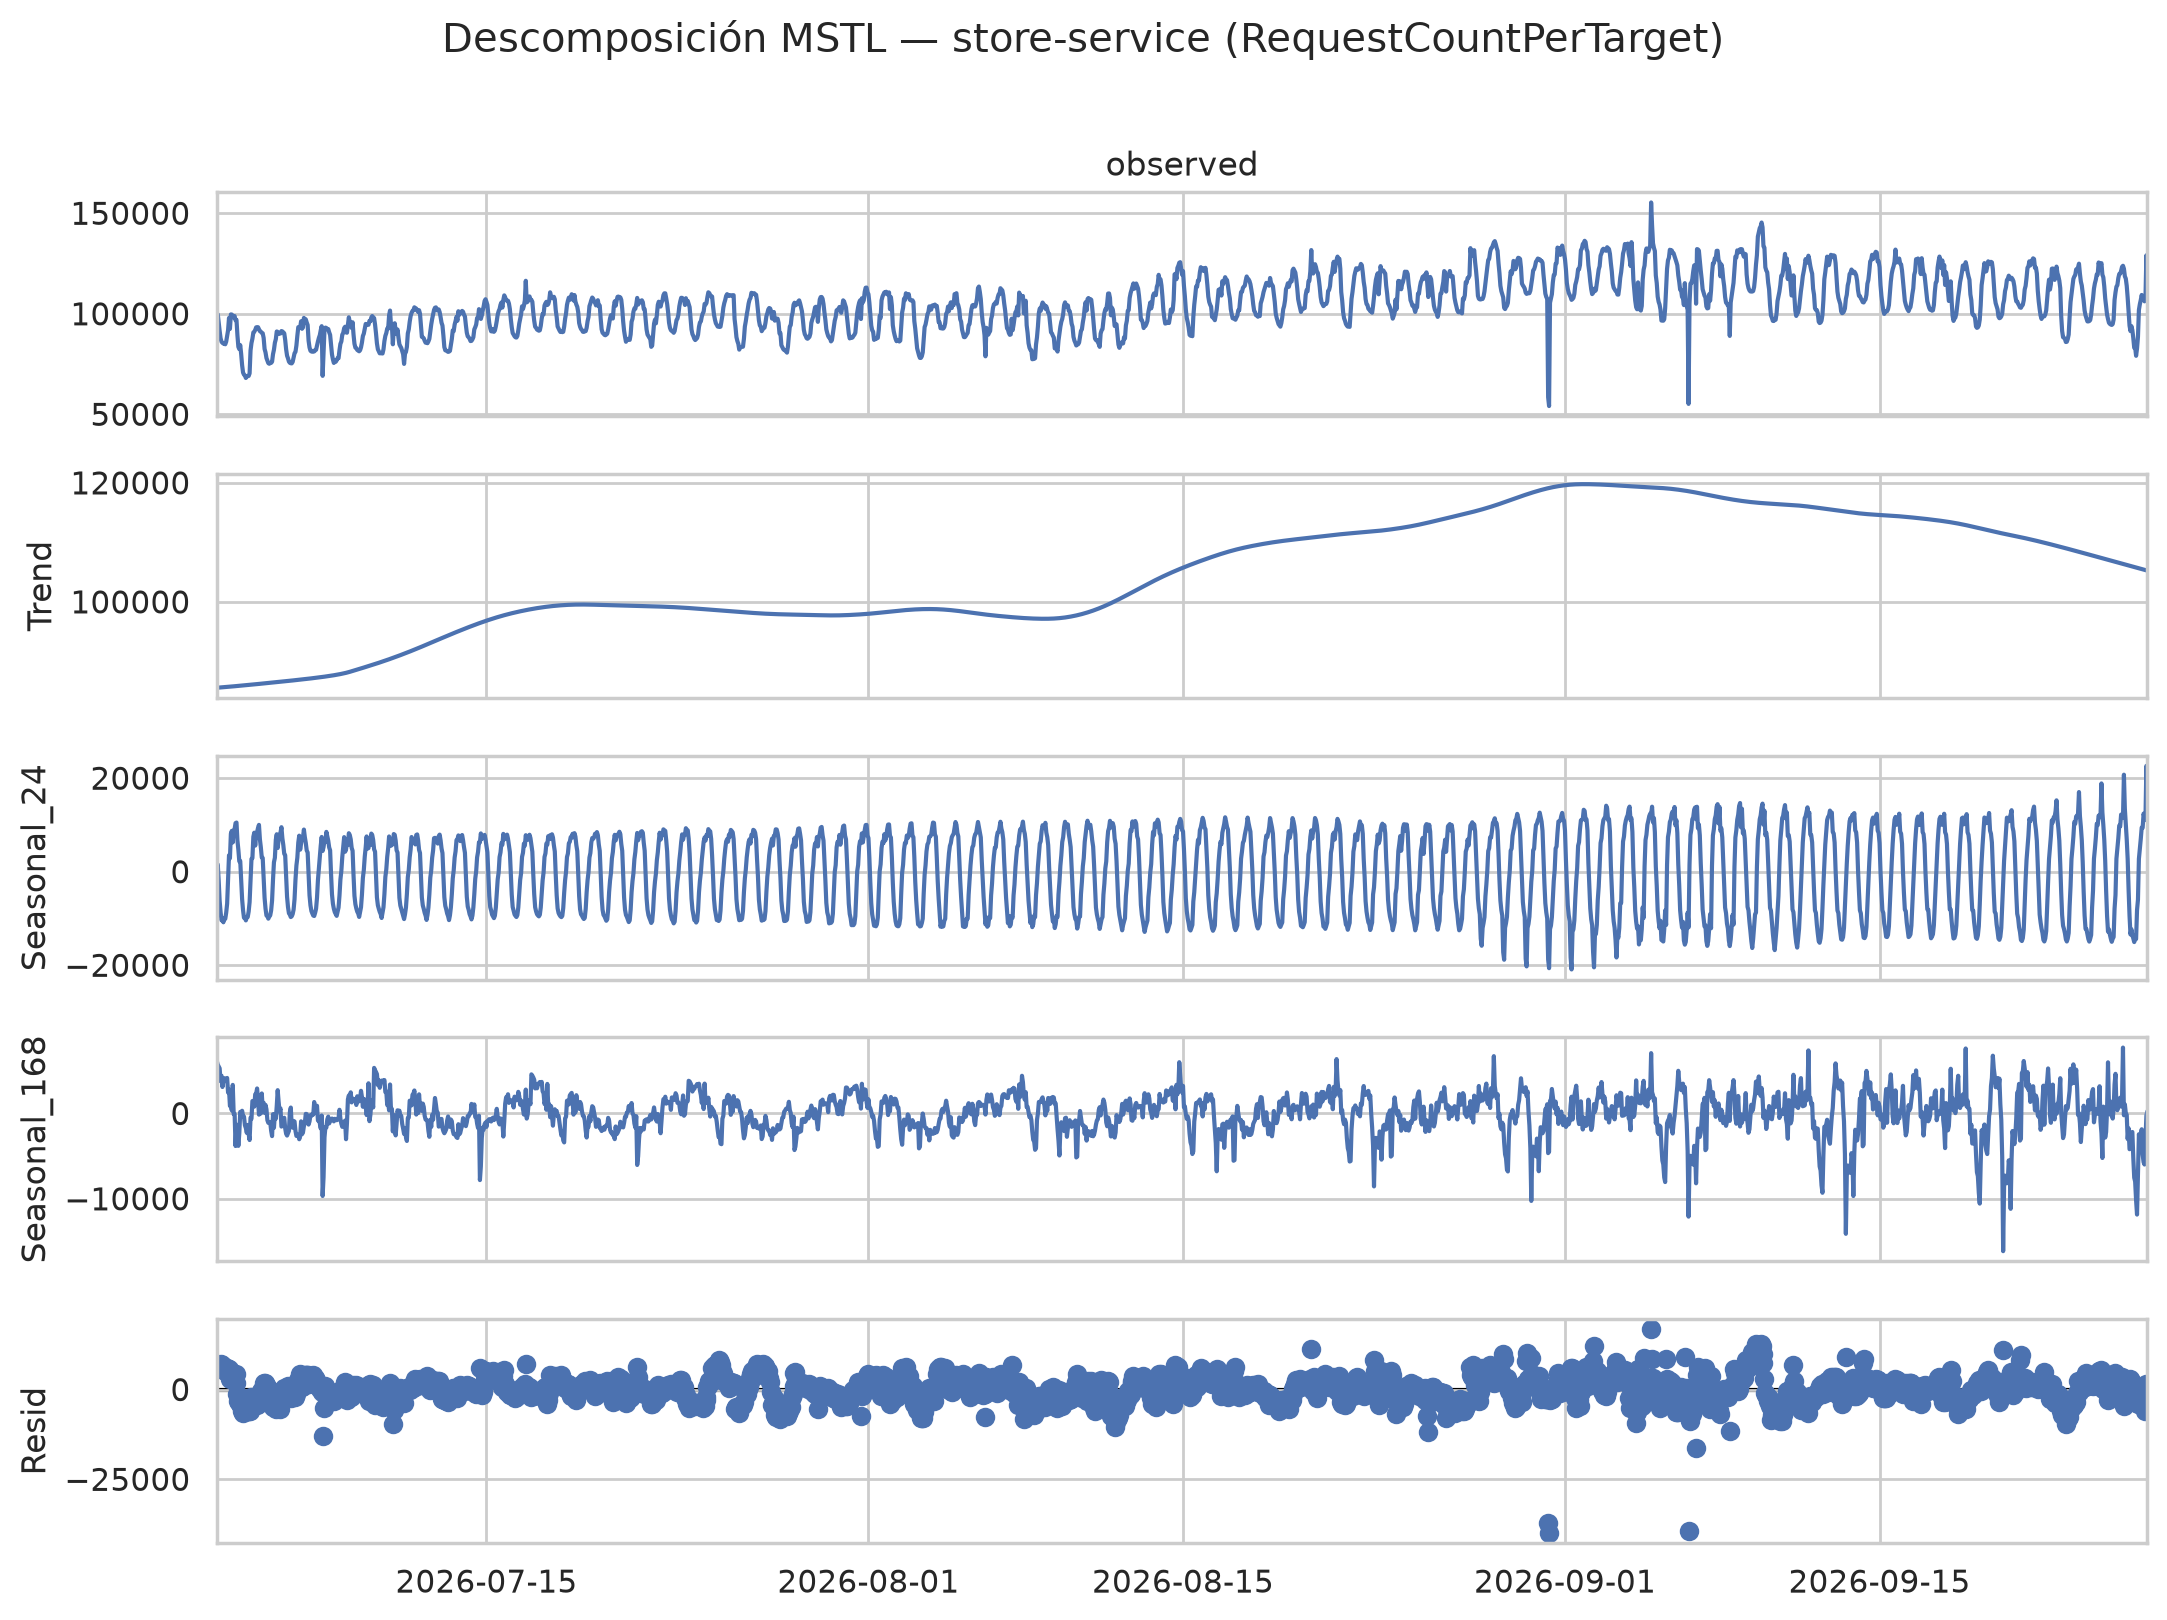
\includegraphics[width=0.85\textwidth]{01_mstl_store_service.png}
  \caption{Descomposición MSTL, serie store-service.}
\end{figure}

\begin{figure}[htbp]
  \centering
  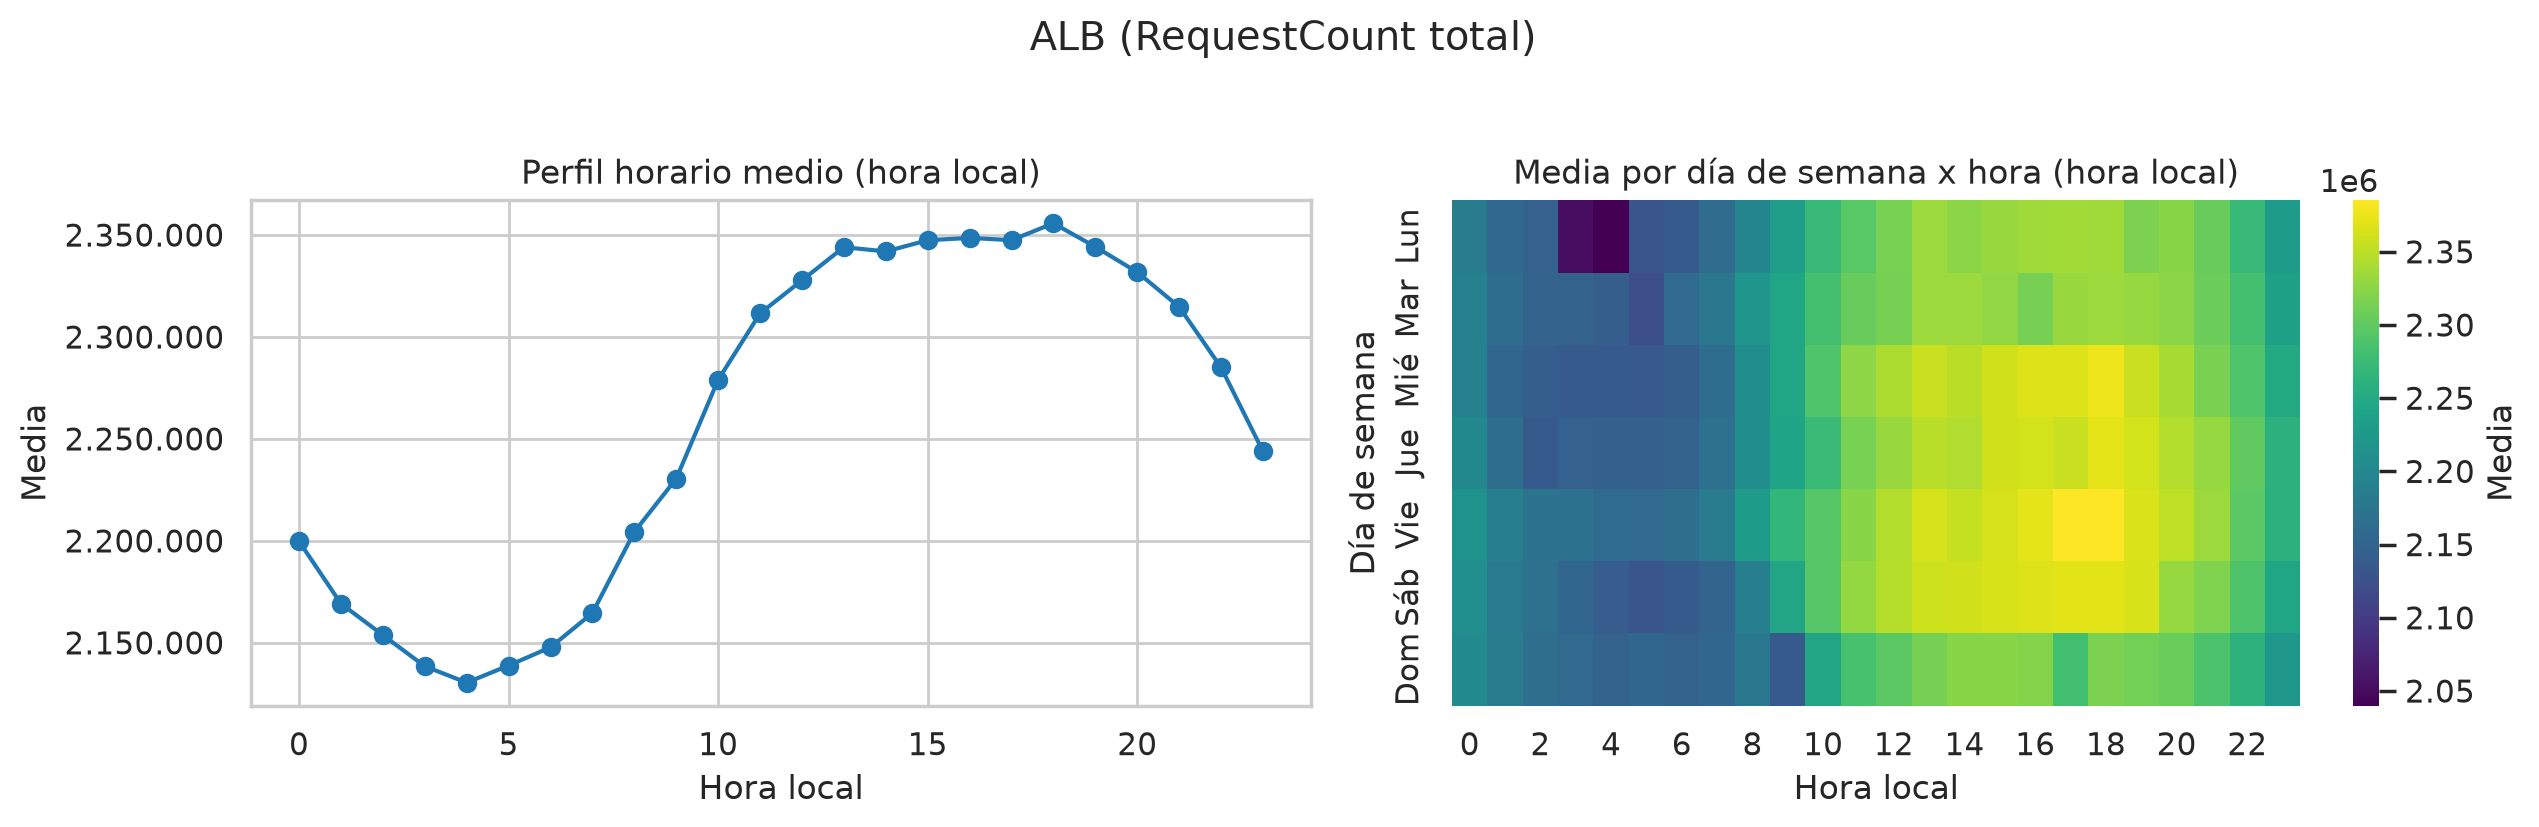
\includegraphics[width=0.8\textwidth]{01_hourly_profile_heatmap_alb.png}
  \caption{Perfil horario por día de la semana (mapa de calor), serie ALB.}
\end{figure}

\begin{figure}[htbp]
  \centering
  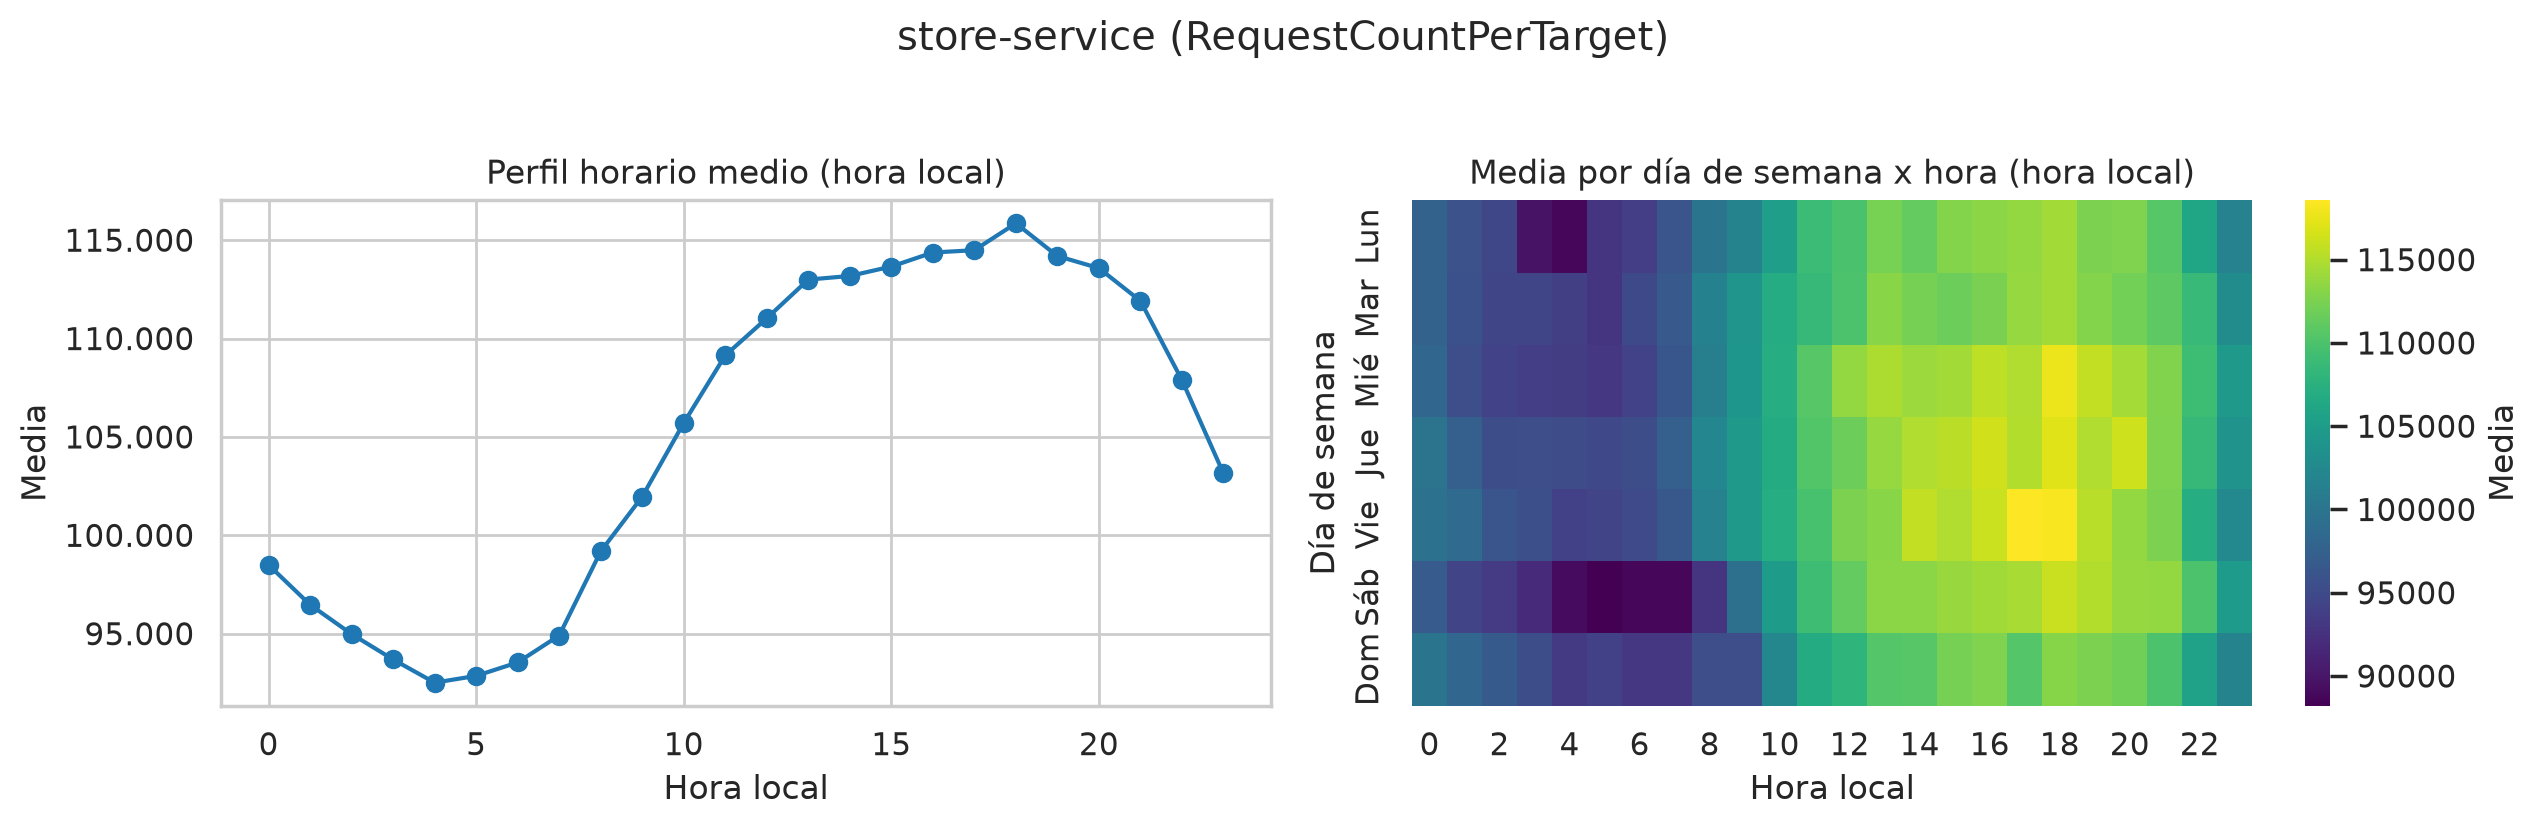
\includegraphics[width=0.8\textwidth]{01_hourly_profile_heatmap_store_service.png}
  \caption{Perfil horario por día de la semana (mapa de calor), serie store-service.}
\end{figure}

\begin{figure}[htbp]
  \centering
  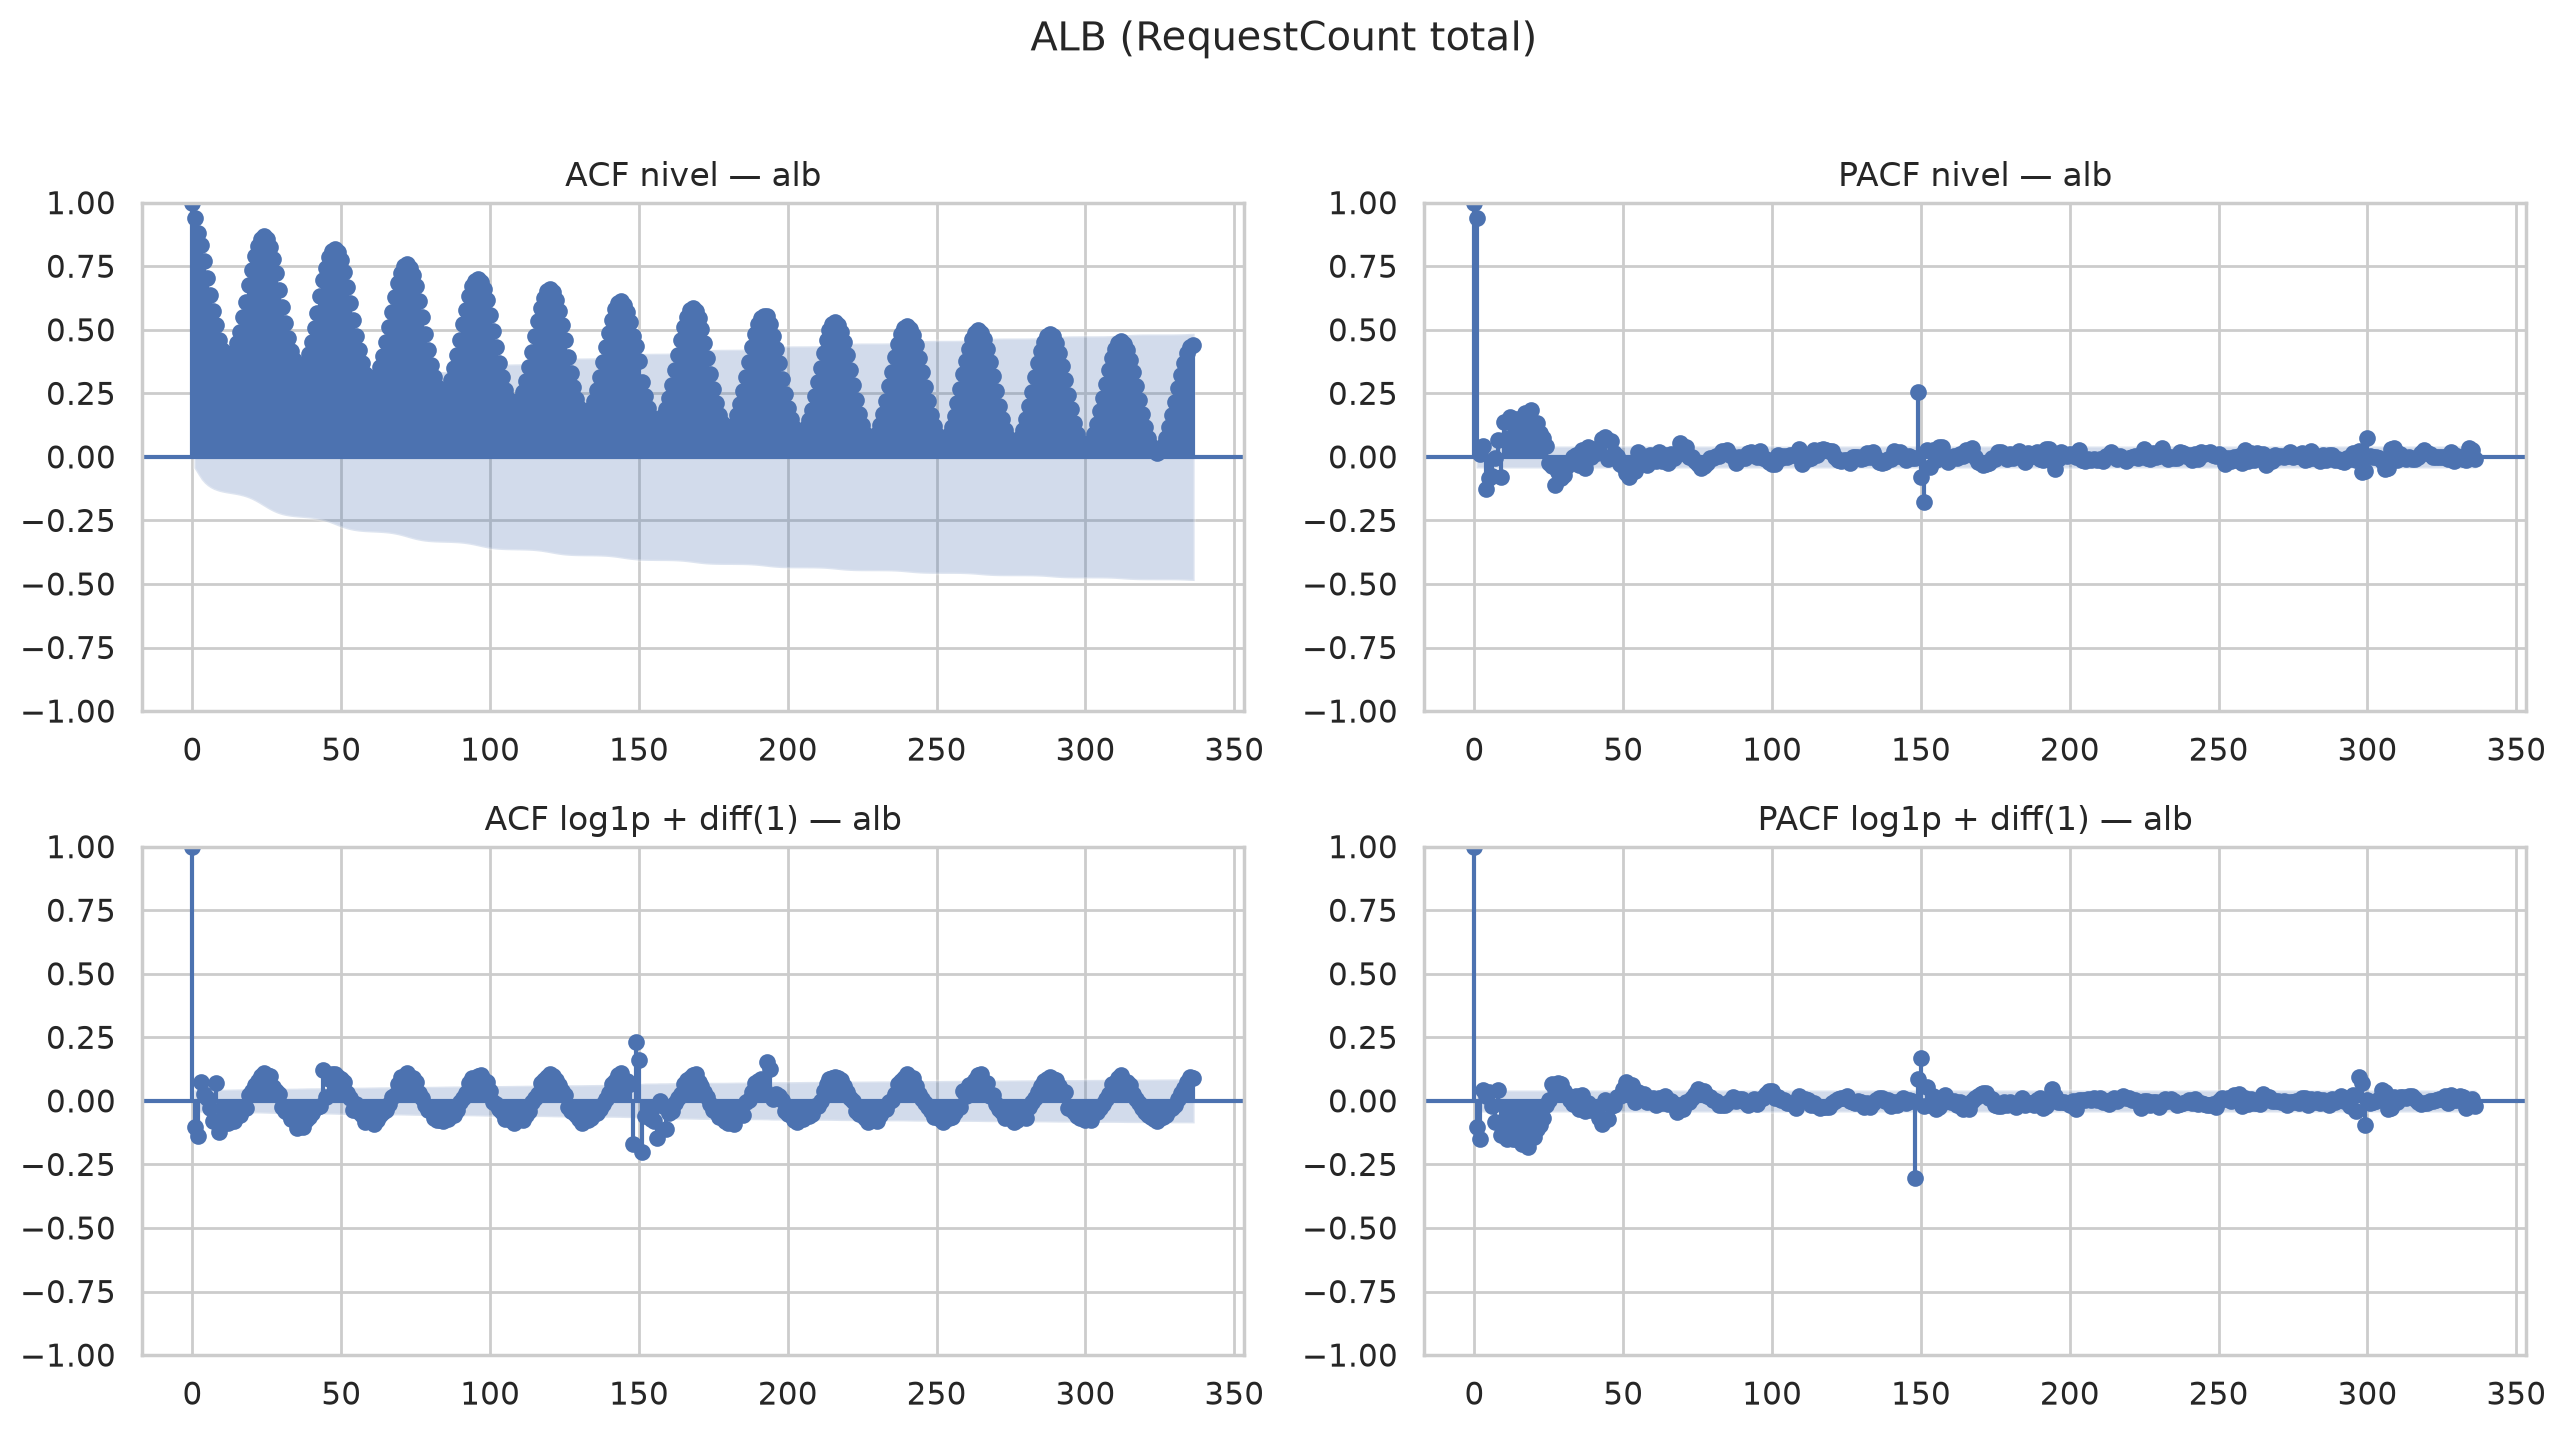
\includegraphics[width=0.75\textwidth]{01_acf_pacf_alb.png}
  \caption{Autocorrelación y autocorrelación parcial, serie ALB.}
\end{figure}

\begin{figure}[htbp]
  \centering
  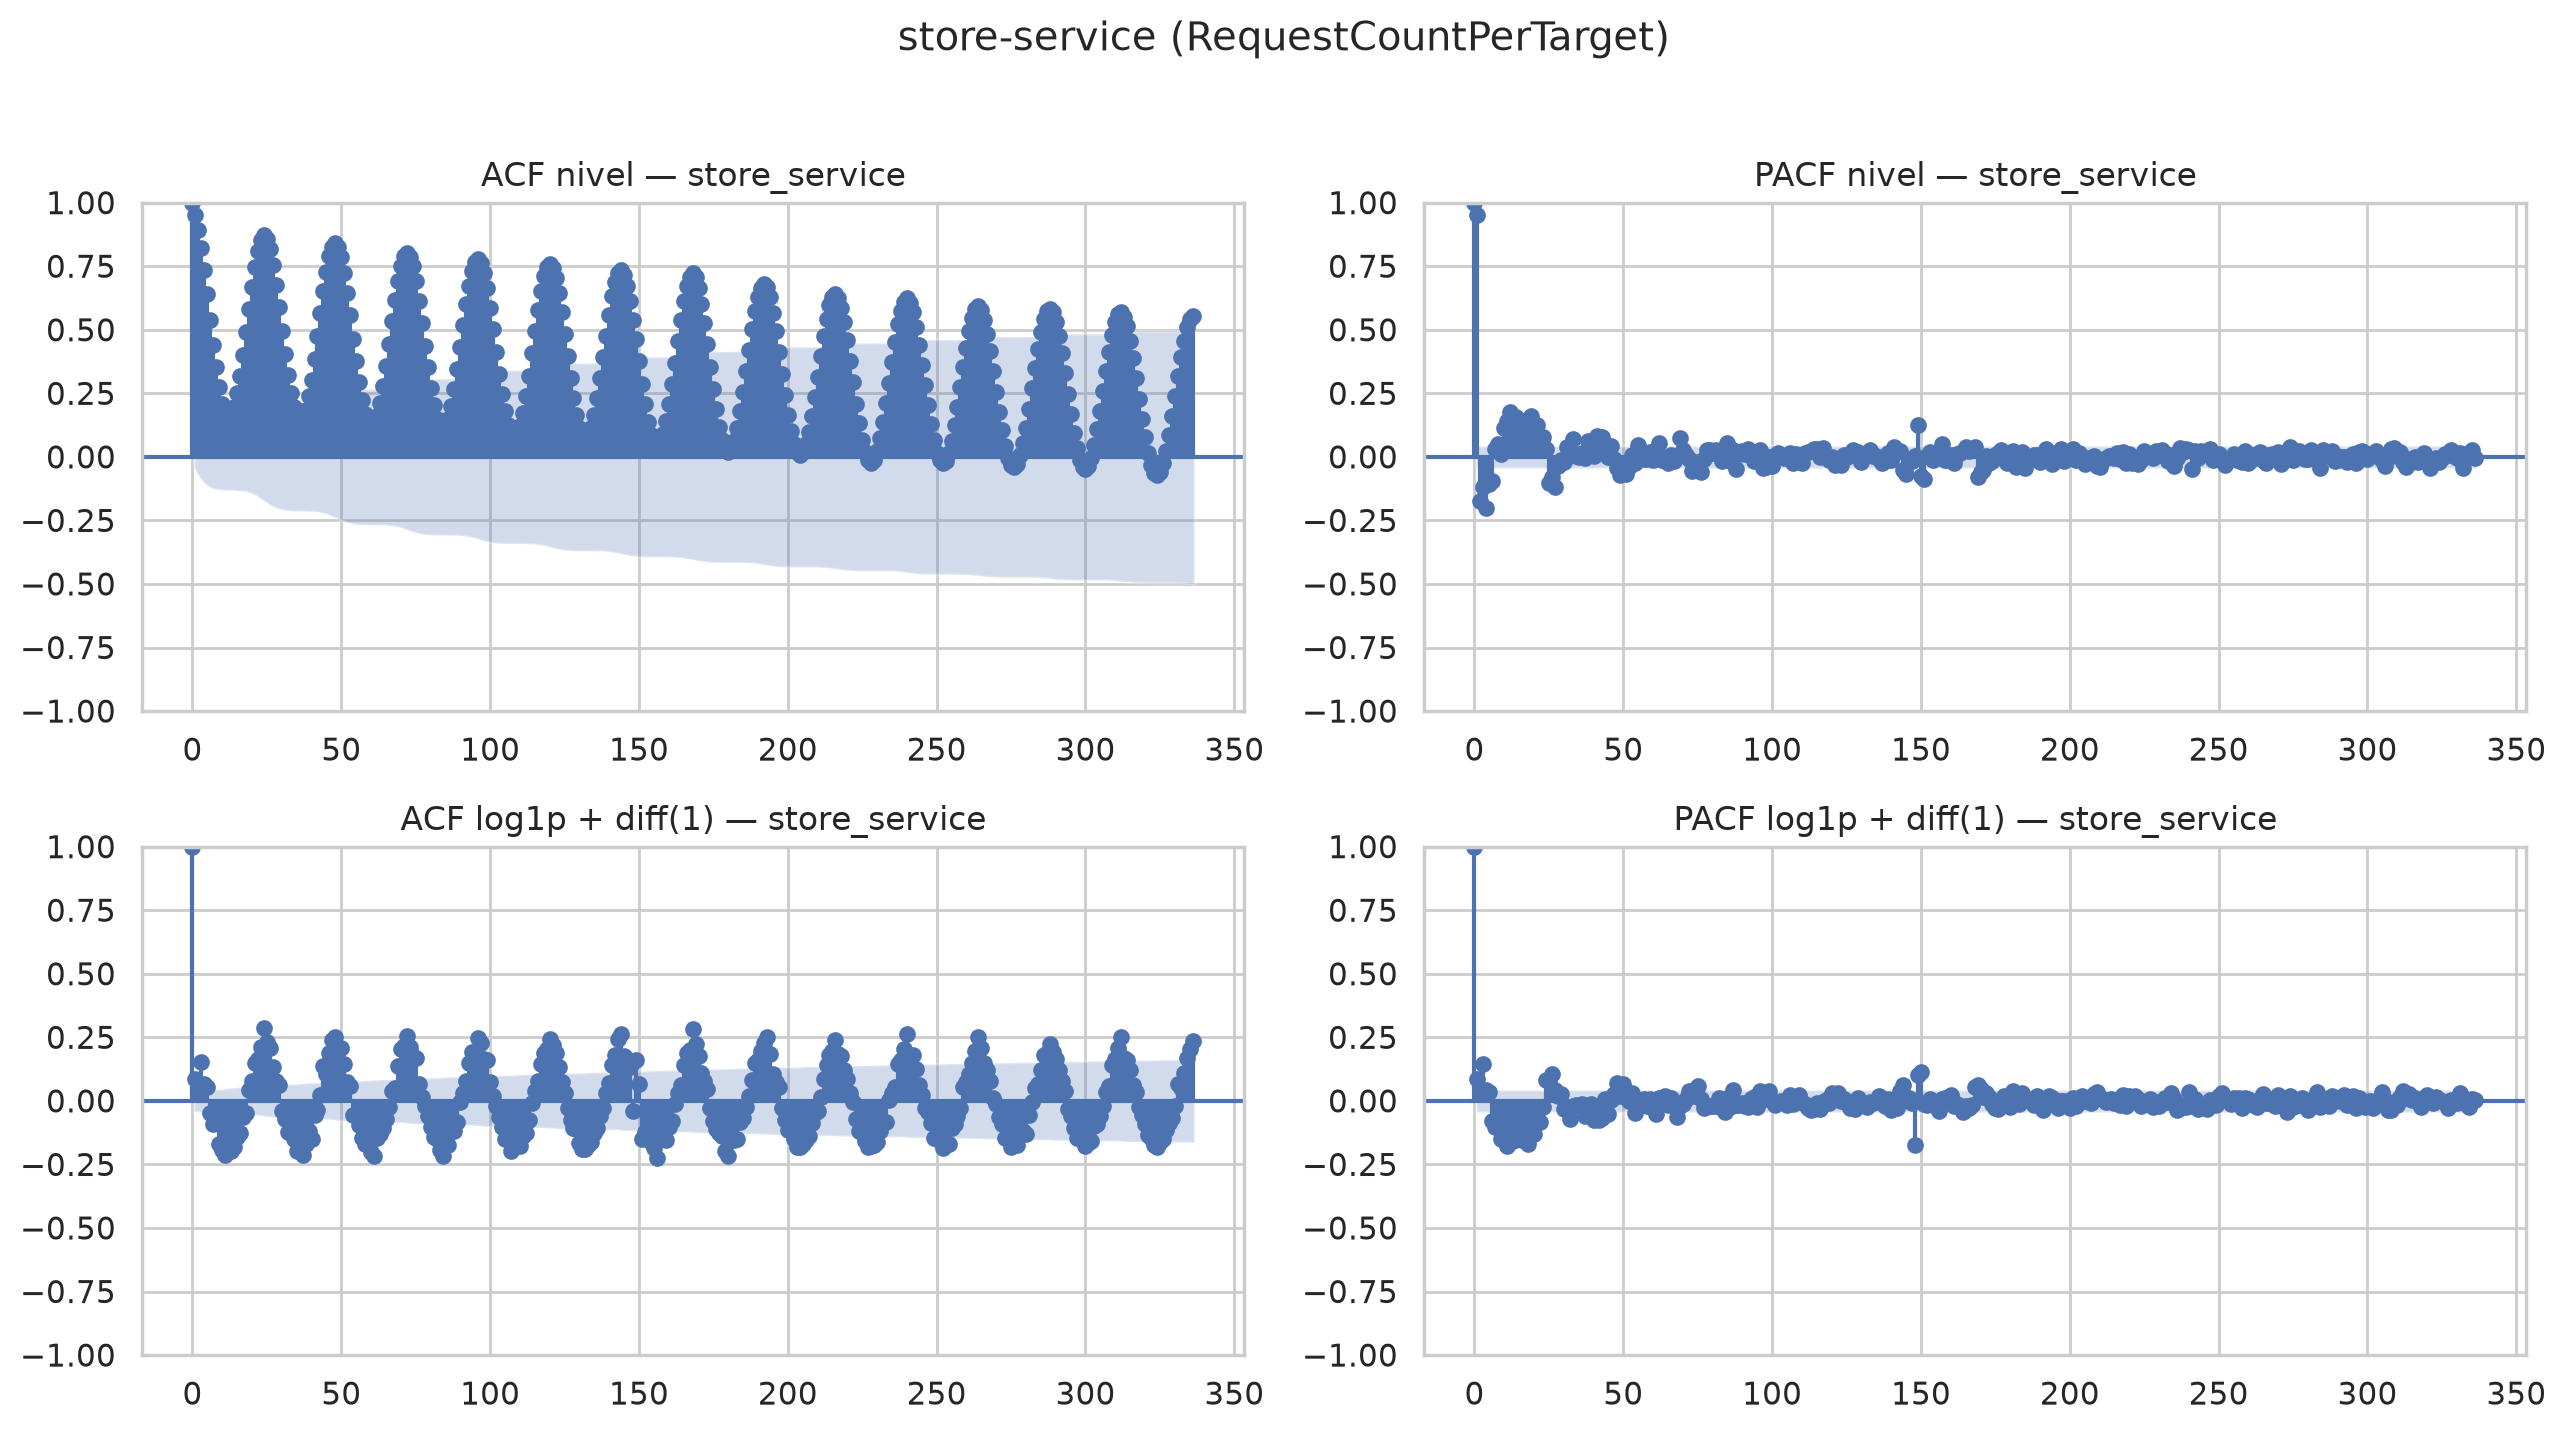
\includegraphics[width=0.75\textwidth]{01_acf_pacf_store_service.png}
  \caption{Autocorrelación y autocorrelación parcial, serie store-service.}
\end{figure}

\begin{figure}[htbp]
  \centering
  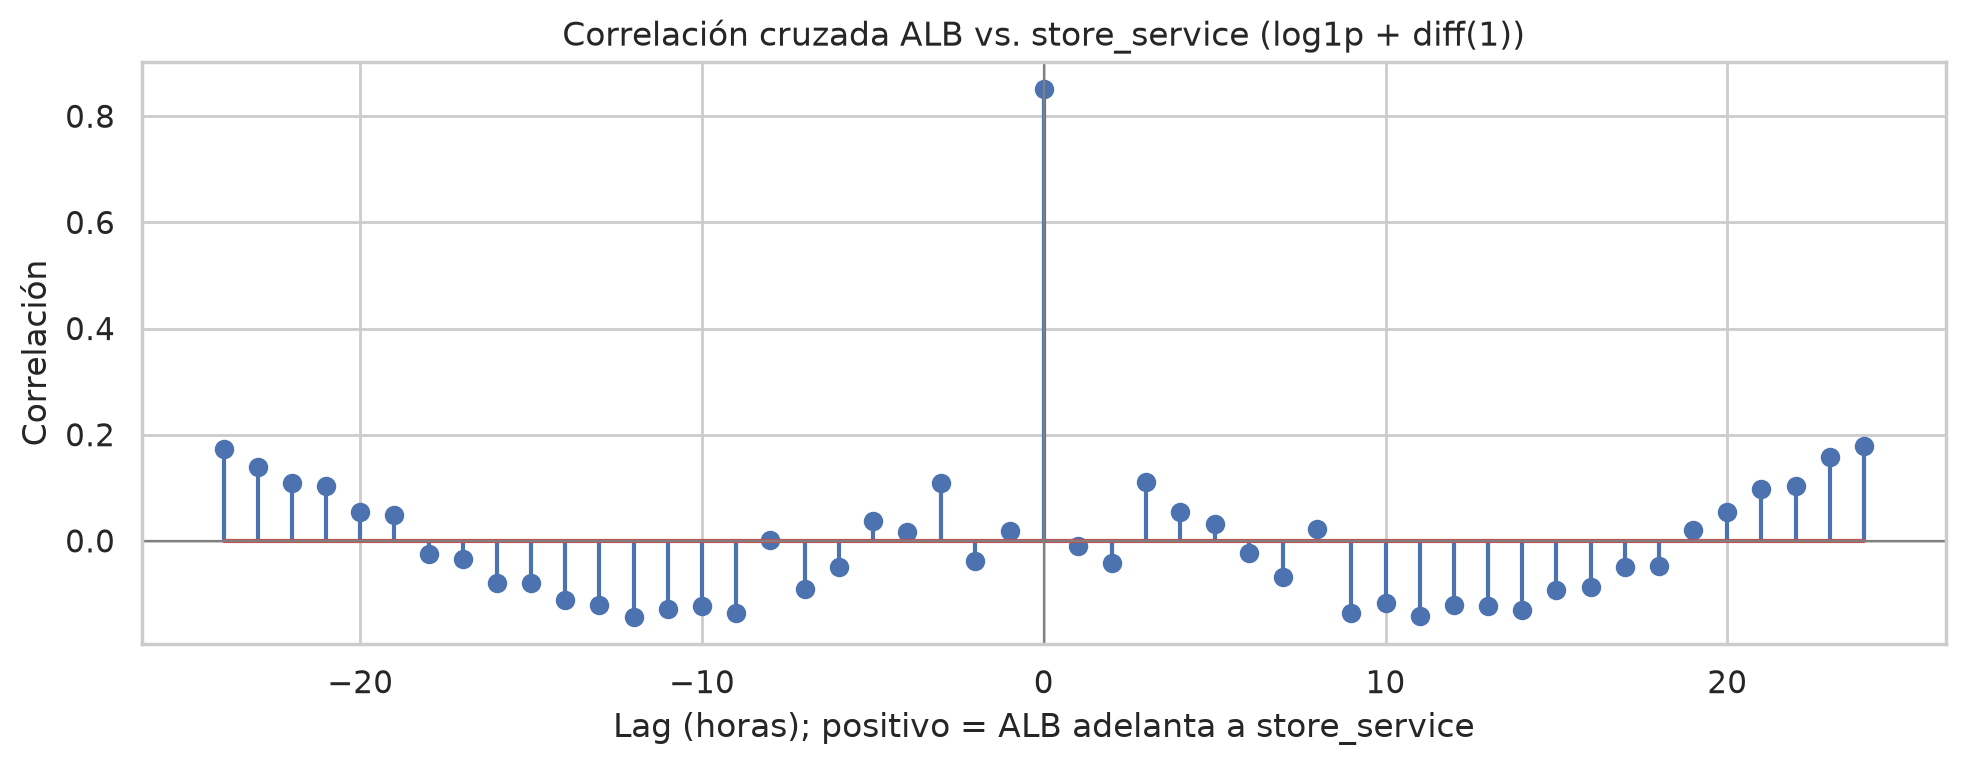
\includegraphics[width=0.75\textwidth]{01_ccf_alb_store_service.png}
  \caption{Correlación cruzada entre ALB y store-service (serie transformada), rezagos de $-24$ a $24$ horas.}
\end{figure}

\begin{figure}[htbp]
  \centering
  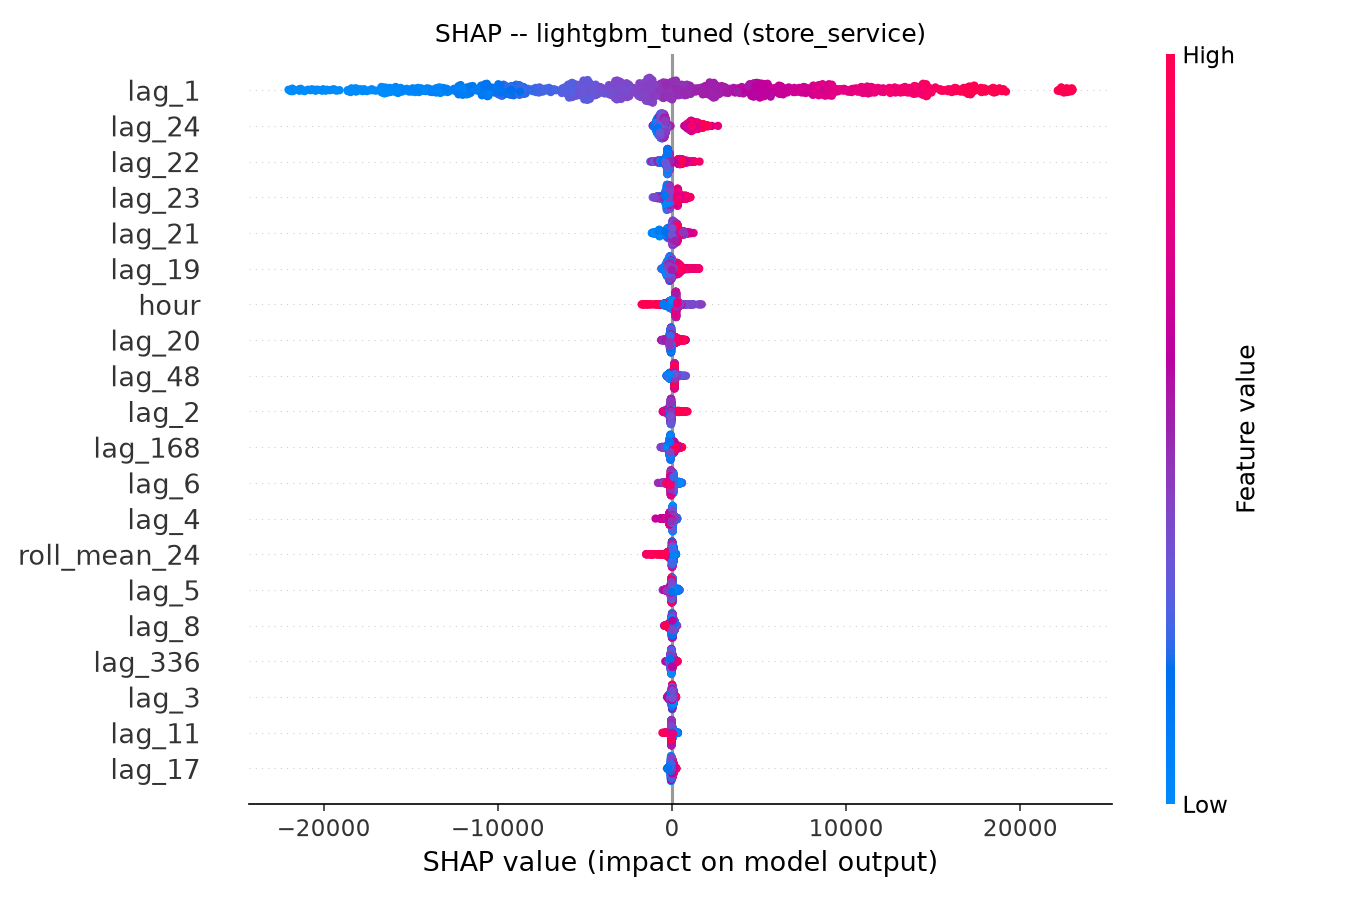
\includegraphics[width=0.85\textwidth]{03_shap_store_service.png}
  \caption{Importancia de variables (SHAP) del mejor modelo de Machine Learning, serie store-service.}
\end{figure}

\begin{figure}[htbp]
  \centering
  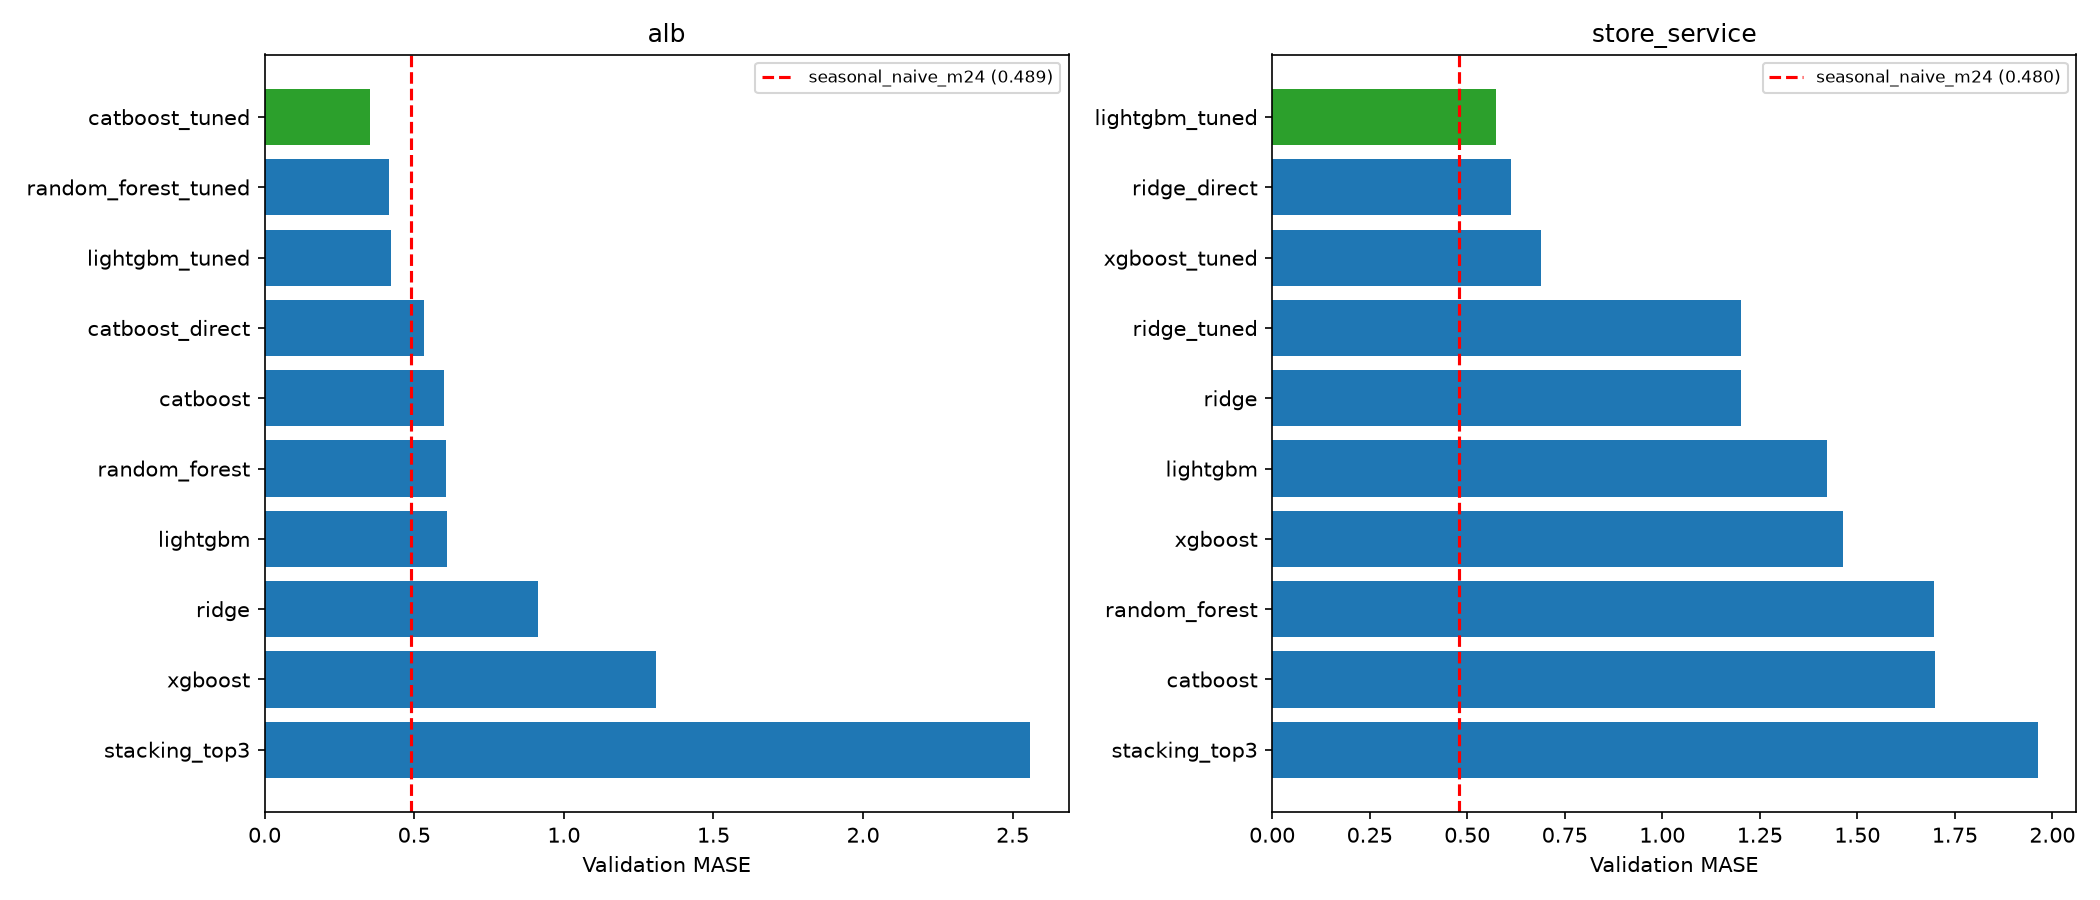
\includegraphics[width=0.85\textwidth]{03_val_mae_ranking.png}
  \caption{MASE de validación, modelos de Machine Learning (fase 03), ambas series.}
\end{figure}

\begin{figure}[htbp]
  \centering
  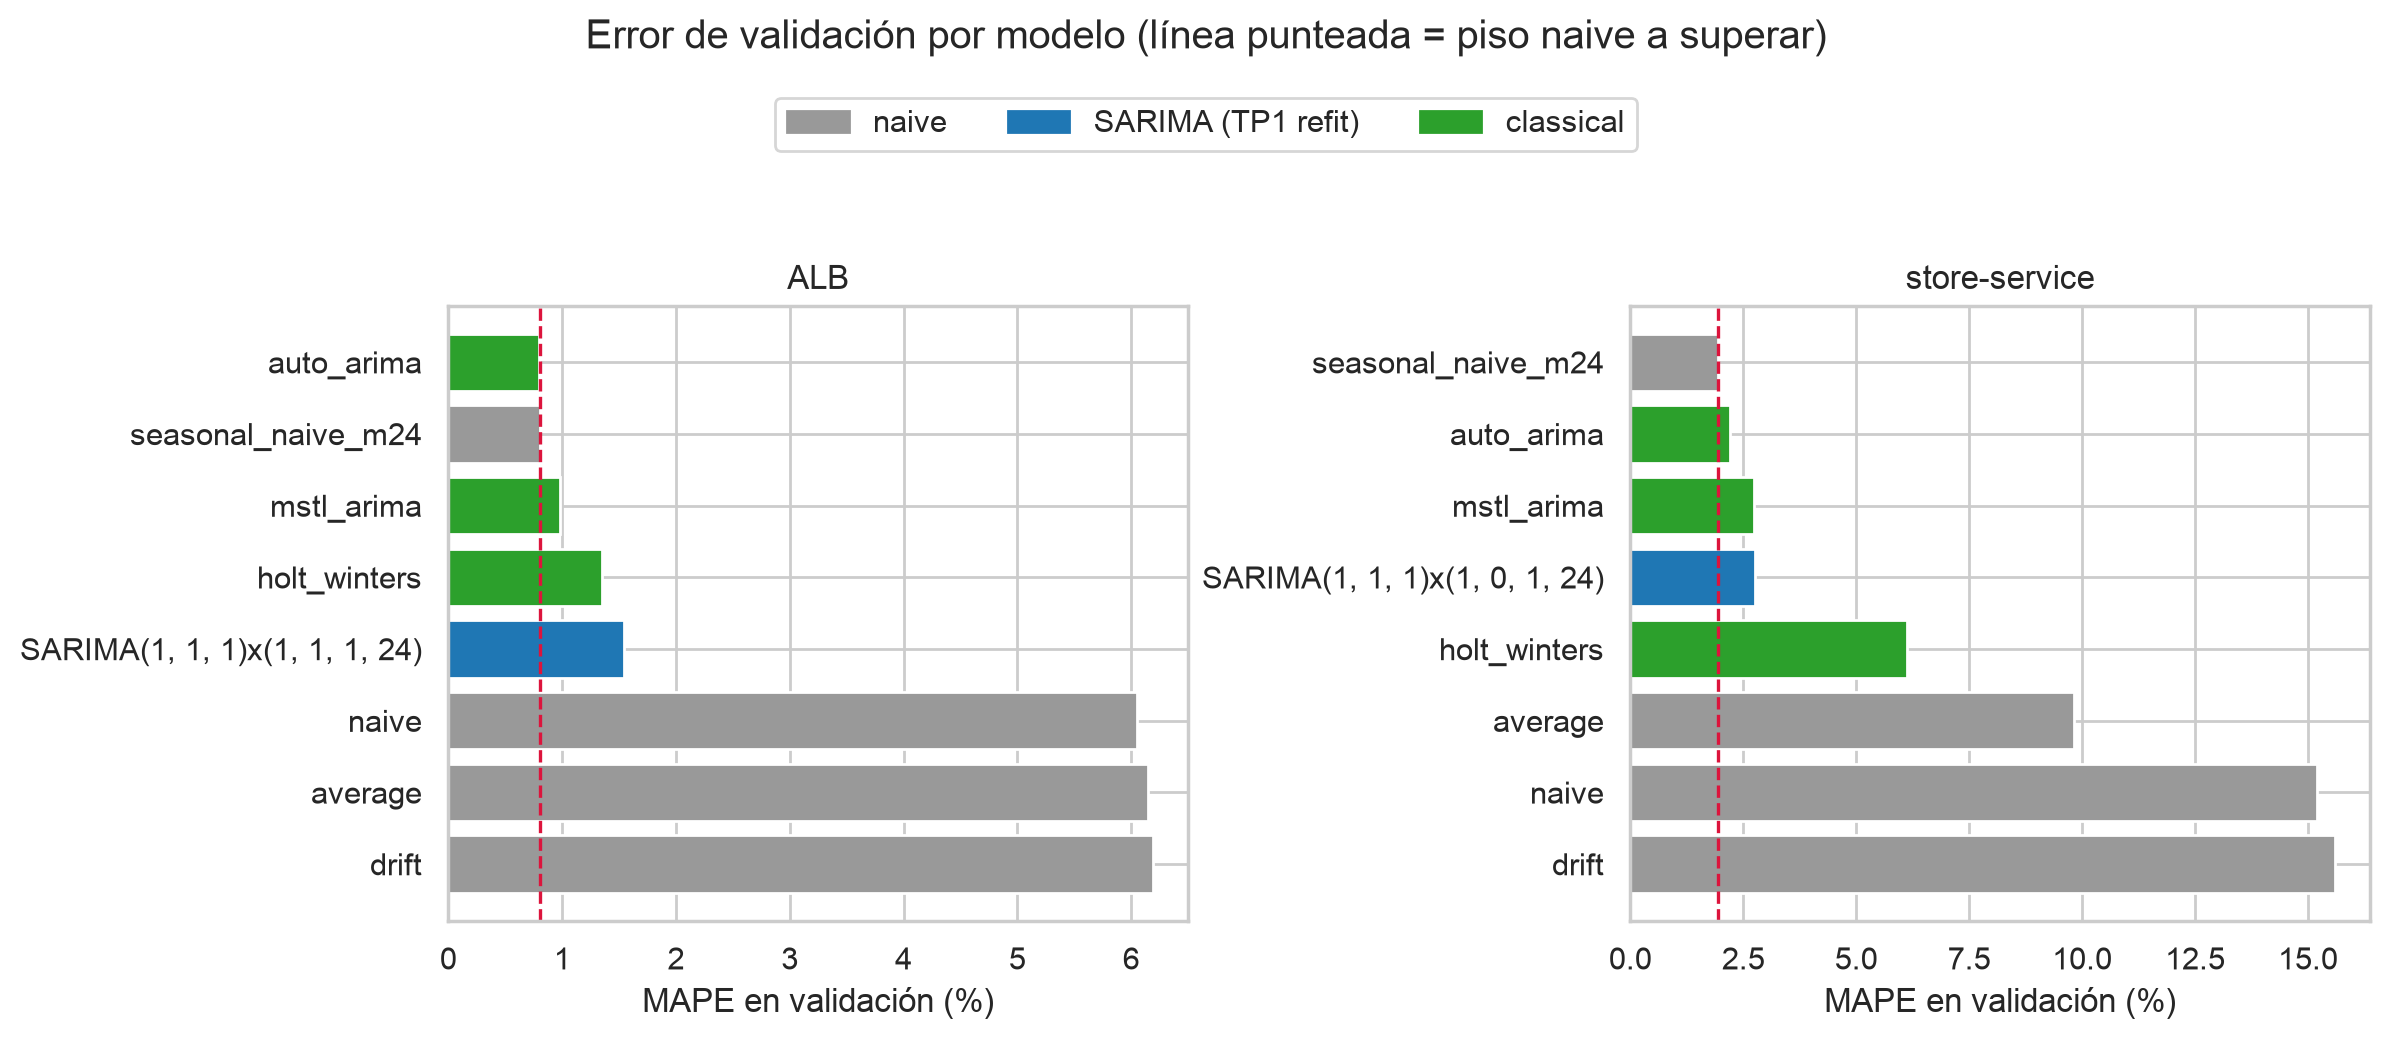
\includegraphics[width=0.85\textwidth]{02_val_mape_ranking.png}
  \caption{MAPE de validación, referencias ingenuas y modelos clásicos (fase 02), ambas series.}
\end{figure}

\begin{figure}[htbp]
  \centering
  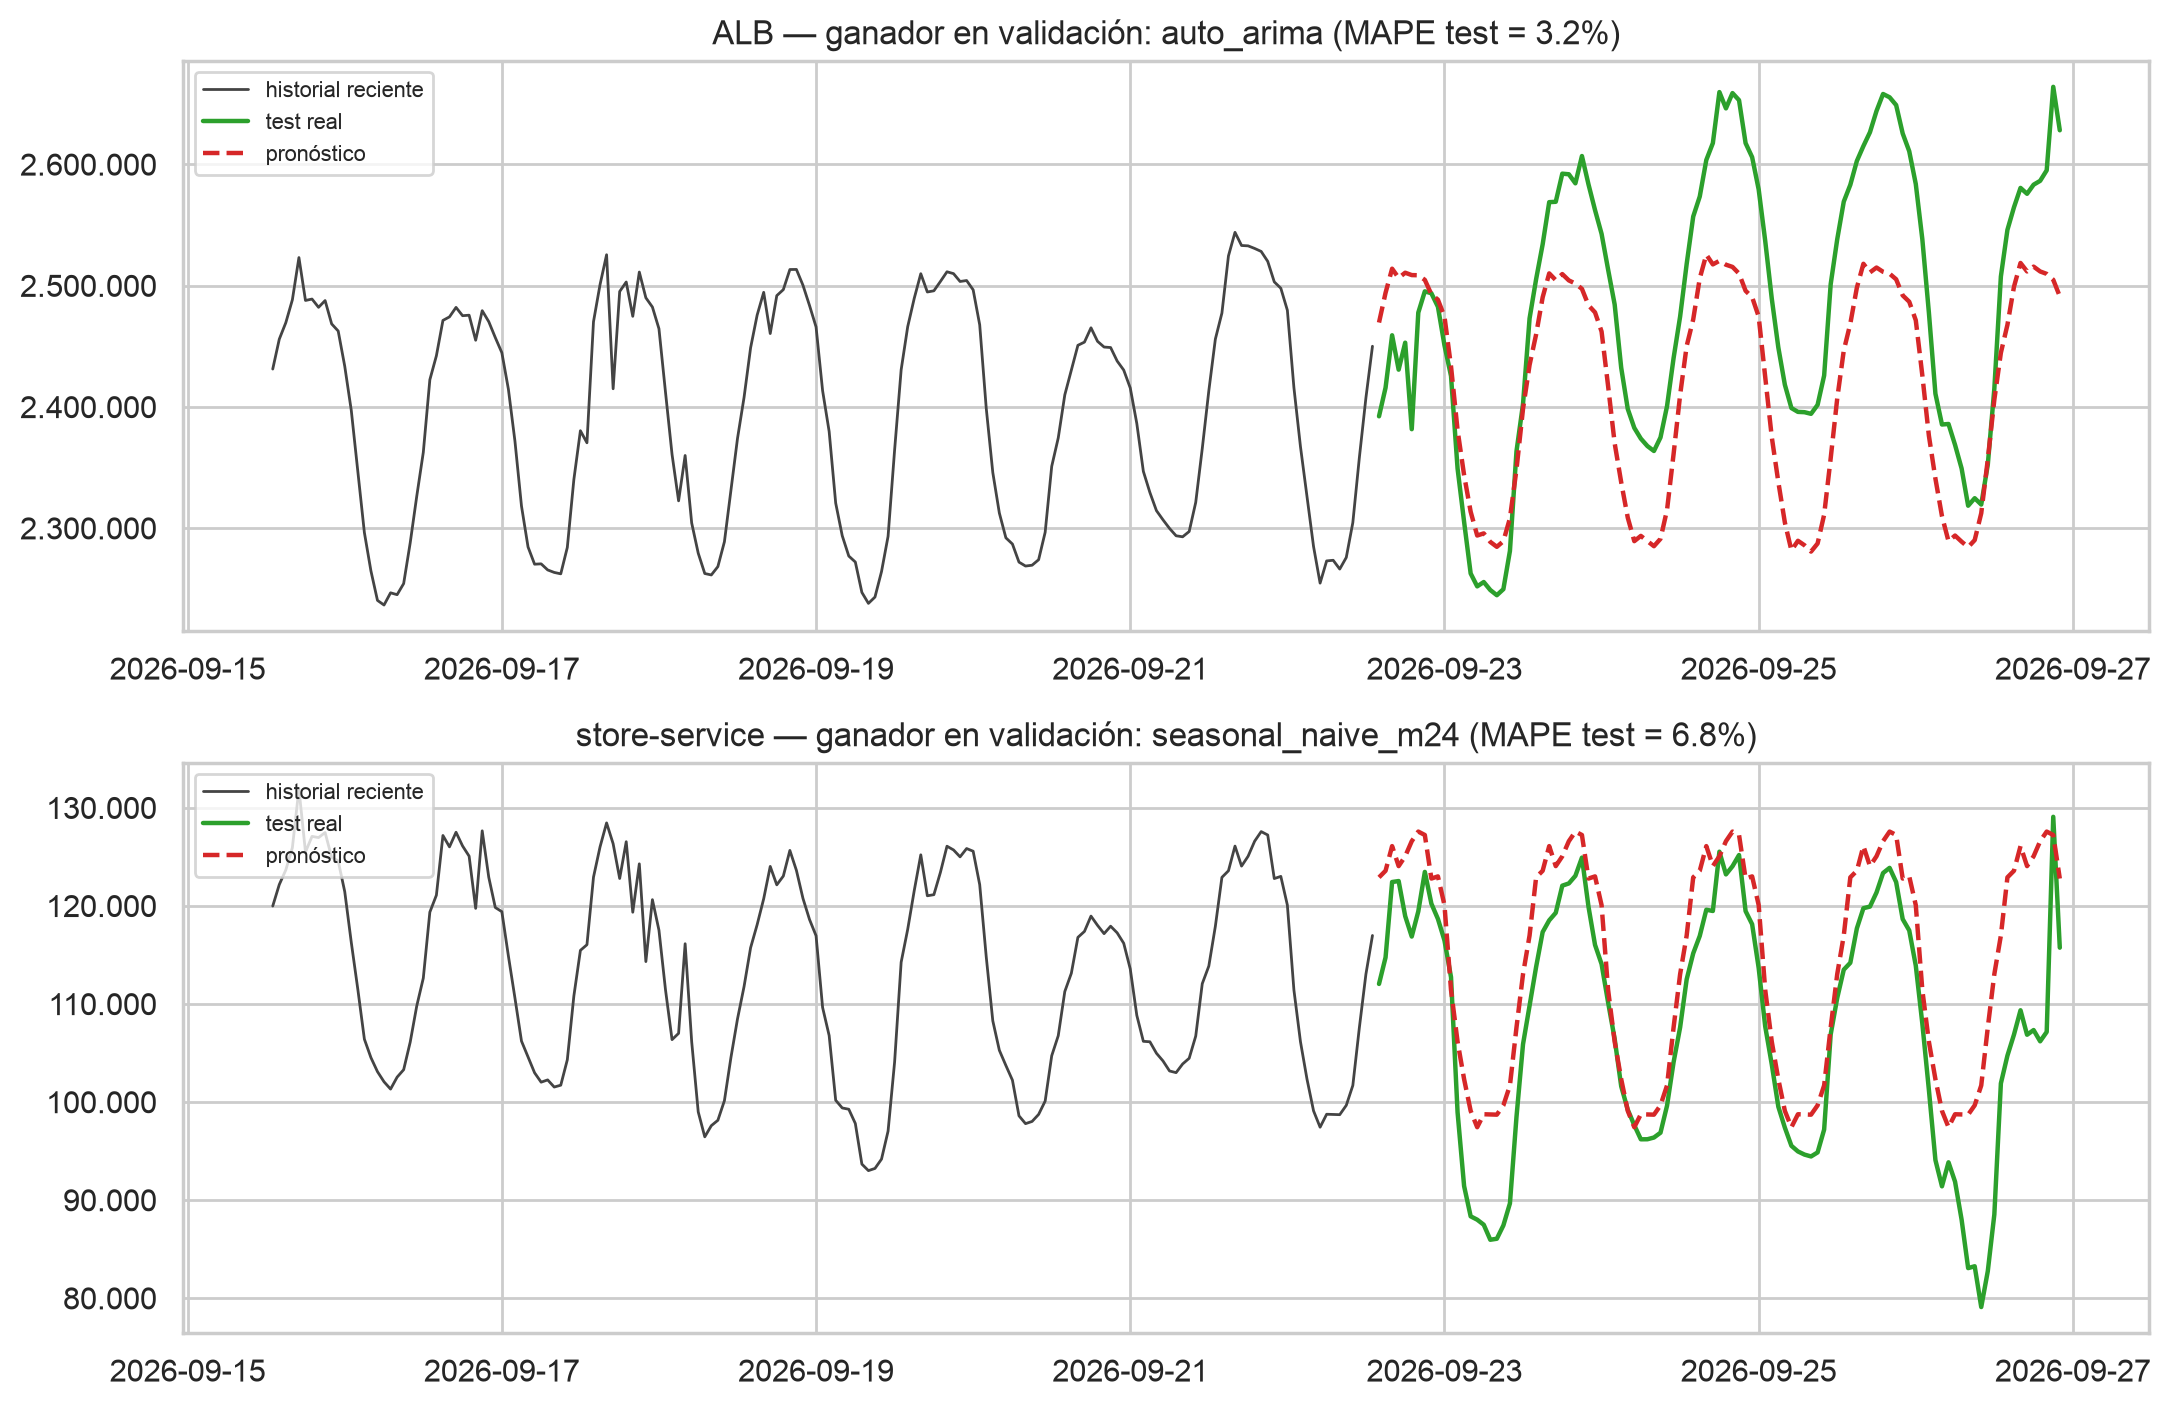
\includegraphics[width=0.9\textwidth]{02_test_forecast_winners.png}
  \caption{Pronóstico de prueba de los mejores modelos de la fase 02, ambas series.}
\end{figure}

\begin{figure}[htbp]
  \centering
  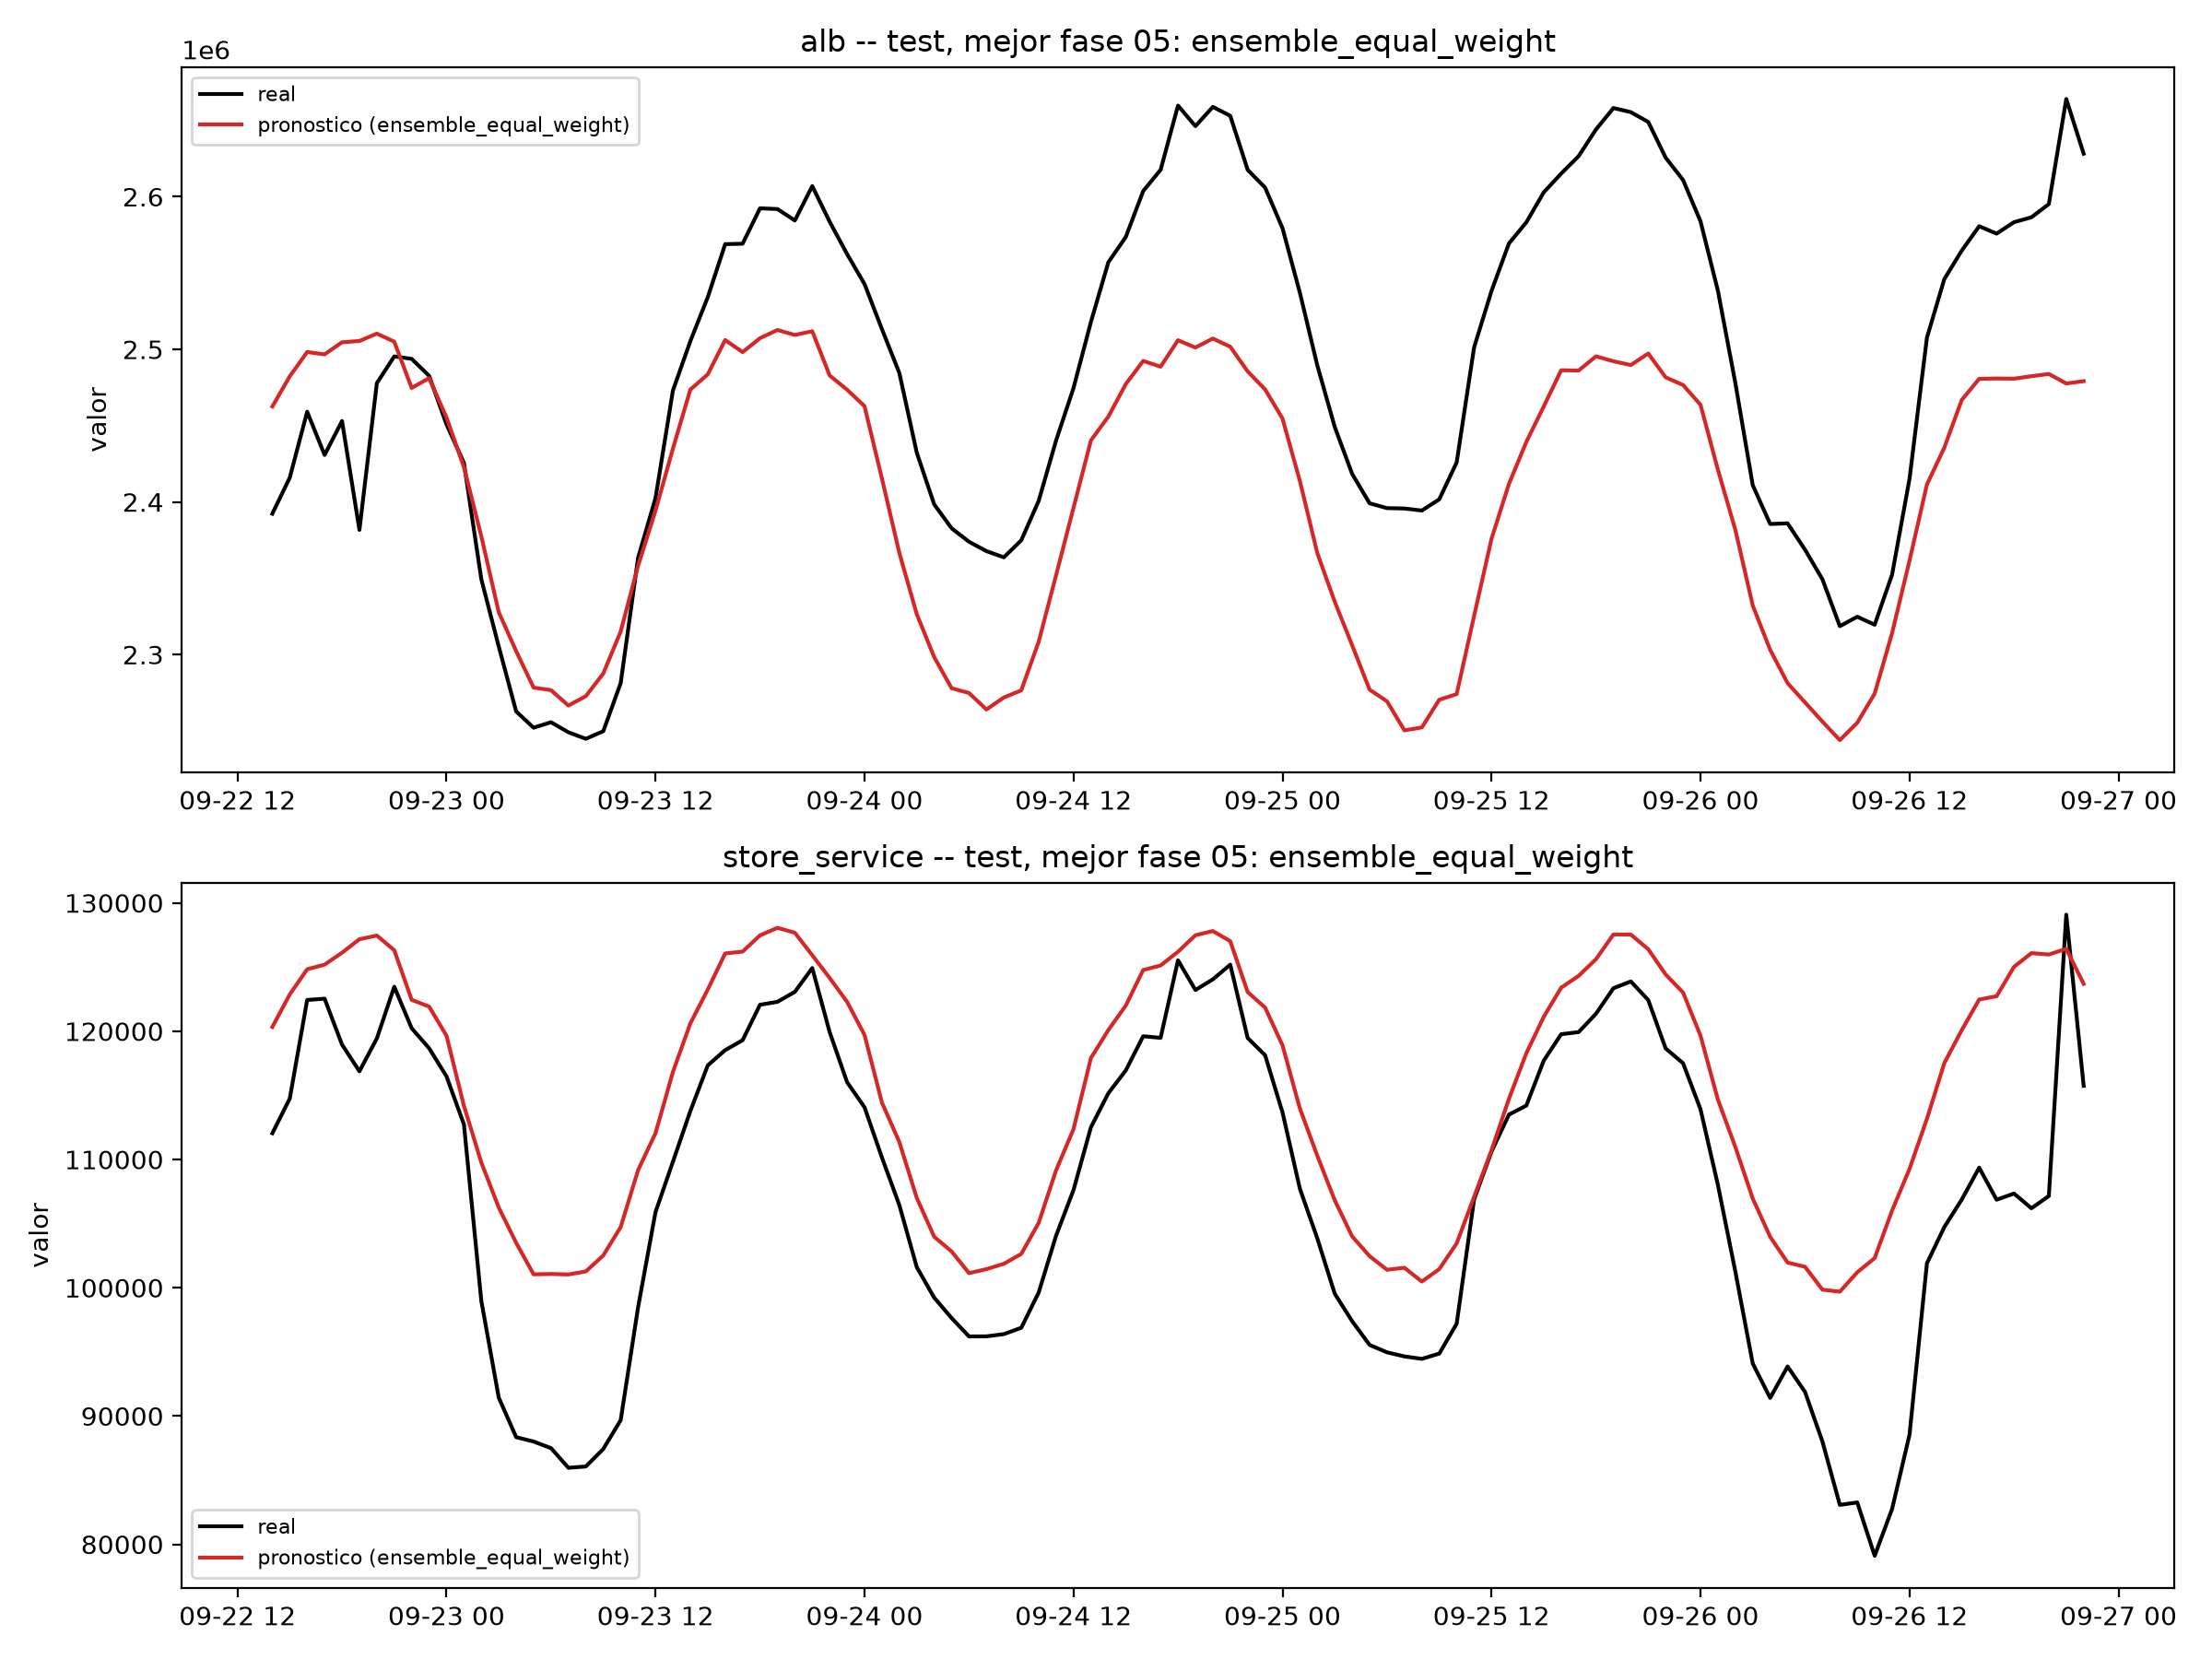
\includegraphics[width=0.9\textwidth]{05_test_forecast_best_model.png}
  \caption{Pronóstico de prueba del mejor modelo de la fase 05 (Prophet, híbridos, AutoML y fundación), ambas series.}
\end{figure}

\section{Apéndice B. Rutinas de cómputo}

Este apéndice reproduce, en forma completa, dos rutinas centrales del protocolo cuyo fragmento se citó de
forma abreviada en el cuerpo del informe: la imputación de la intervención de despliegue y el cálculo del
conjunto de flags de contaminación utilizado por la regla de selección.

\begin{lstlisting}[caption={Imputación de la ventana de intervención mediante el valor de la semana anterior corregido por nivel (\texttt{tsa\_final/data.py}).}]
def impute_intervention(series: pd.Series, start: pd.Timestamp, end: pd.Timestamp) -> pd.Series:
    """Reemplaza [start, end] por el valor de t-168h, corregido por la razon
    entre el nivel de la semana previa a la intervencion y el de la semana
    anterior a esa. Preserva el crecimiento organico semana a semana en lugar
    de asumir que el nivel pre-intervencion se repite sin cambios."""
    pre_window = series.loc[start - pd.Timedelta(hours=168):start - pd.Timedelta(hours=1)]
    prior_week = series.loc[start - pd.Timedelta(hours=336):start - pd.Timedelta(hours=169)]
    ratio = pre_window.mean() / prior_week.mean()

    imputed = series.copy()
    mask = (series.index >= start) & (series.index <= end)
    imputed.loc[mask] = series.shift(168).loc[mask] * ratio
    return imputed
\end{lstlisting}

\begin{lstlisting}[caption={Marcado de modelos con puntaje de validación contaminado (\texttt{tsa\_final/selection.py}).}]
CONTAMINATED_MODELS = {
    "catboost_tuned": _TUNED_REASON,
    "random_forest_tuned": _TUNED_REASON,
    "lightgbm_tuned": _TUNED_REASON,
    "ridge_tuned": _TUNED_REASON,
    "xgboost_tuned": _TUNED_REASON,
    "stacking_top3": _STACKING_REASON,
    "ensemble_equal_weight": _ENSEMBLE_REASON,
    # prophet_tuned se ajusta sobre una ventana segura de 168h, no sobre la
    # ventana de validacion: no se marca como contaminado.
}

def add_contamination_flags(pool: pd.DataFrame) -> pd.DataFrame:
    pool = pool.copy()
    pool["val_contaminated"] = pool["model"].isin(CONTAMINATED_MODELS)
    pool["contamination_reason"] = pool["model"].map(CONTAMINATED_MODELS).fillna("")
    return pool

def eligible_val(pool: pd.DataFrame, series: str) -> pd.DataFrame:
    """Modelos elegibles para seleccion: split == 'val' y no contaminados,
    ordenados por MAE de validacion ascendente."""
    mask = (pool["series"] == series) & (pool["split"] == "val") & (~pool["val_contaminated"])
    return pool.loc[mask].sort_values("MAE")
\end{lstlisting}

\pendiente{Serie 3 (a cargo de otro integrante del grupo). El material gráfico y las tablas completas
correspondientes a esta serie se incorporarán en este apéndice una vez completado su análisis.}


\end{document}
